%!TEX TS-program = xelatex
%!TEX encoding = UTF-8 Unicode
\documentclass[a4paper, 12pt, oneside]{book}

\usepackage{cite}
%\usepackage{chapterbib}
%The chapterbib package facilitates multiple bibliographies in a LATEX document
\usepackage[hyphens]{url}
%Verbatim with URL-sensitive line breaks.
\usepackage[colorlinks=true,linkcolor=black,citecolor=black,filecolor=blue,urlcolor=blue,unicode]{hyperref}
%The hyperref package is used to handle cross-referencing commands in LaTeX to produce hypertext links in the document. The package provides backends for the \special set defined for HyperTeX DVI processors; for embedded pdfmark commands for processing by Acrobat Distiller (dvips and Y&Y’s dvipsone); for Y&Y’s dviwindo; for PDF control within pdfTeX and dvipdfm; for TeX4ht; and for VTeX’s pdf and HTML backends.
\usepackage{verbatim}
%The verbatim environment  simply reproduces every character you input, including all  s p a c e s!
\usepackage{color}
%you can set the color of the font of the text, and set the background color of the page.
\usepackage[dvipsnames]{xcolor}
%xecolor package is a simple package which defines about 140 different colors by XeTeX's font
\usepackage{graphicx}
%Standard LaTeX graphics.
\usepackage{array}
%The array environment is used to make a table of information, with column alignment (left, center, or right) and optional vertical lines separating the columns.
%\usepackage{gensymb}
%Provides generic commands \degree, \celsius, \perthousand, \micro and \ohm which work both in text and maths mode.
\usepackage{indentfirst}
%Make the first line of all sections etc., be indented by the usual paragraph indentation. This should work with all the standard document classes. This minimalist package is part of the "tools" bundle in the LaTeX required distribution.
%\usepackage{algorithm}
\usepackage[linesnumbered,boxed]{algorithm2e}
\usepackage{algpseudocode}
%A suite of tools for typesetting algorithms in pseudo-code. The algorithmicx package provides many possibilities to customize the layout of algorithms. You can use one of the predefined layouts (pseudocode, pascal and c and others), with or without modifications, or you can define a completely new layout for your specific needs.
\usepackage{enumitem}
%Control layout of itemize, enumerate, description.  It supersedes both enumerate and mdwlist (providing well- structured replacements for all their funtionality), and in addition provides functions to compute the layout of labels, and to 'clone' the standard environments, to create new environments with counters of their own.
\usepackage{mfirstuc}
%\makefirstuc{〈stuff 〉} This makes the first object of 〈stuff 〉 uppercase unless 〈stuff 〉 starts with a con- trol sequence followed by a non-empty group, in which case the first object in the group is converted to uppercase.
\usepackage{fancyvrb}
%This package provides very sophisticated facilities for reading and writing ver- batim TEX code.
\usepackage{amsfonts}
%TeX fonts from the American Mathematical Society.
\usepackage{ifmtarg}
%If-then-else command for processing potentially empty arguments.
\usepackage{amsmath}
%The amsmath package is a LATEX package that provides miscellaneous enhance- ments for improving the information structure and printed output of documents that contain mathematical formulas.
\usepackage{amssymb}
% Math symbols
\usepackage[mathcal]{euscript}
%This file sets up some font shape definitions to use the Euler script symbols in math mode.
\usepackage[notbib]{tocbibind}
%Add (or disable) bibliography/index/contents to Table of Contents.
\usepackage{rotating}
%Rotation tools, including rotated full-page floats.
\usepackage{hhline}
%The command \hhline produces a line like \hline, or a double line like \hline\hline, except for its interaction with vertical lines. The command takes a preamble (rather like the preamble of a tabular environment), and this specifies whether there are to be one or two horizontal lines, and what happens when the horizontal line meets a vertical one. The package is part of the tools bundle in the LaTeX required distribution.
\usepackage{wallpaper}
%Easy addition of wallpapers (background images) to LaTeX documents, including tiling.
\usepackage{pdfpages}
%Include PDF documents in LaTeX.

% For multiple figures
\usepackage{subcaption}
% For fix the table in the section.
\usepackage{float}

%Define \XeTeX \XeLaTeX command
\def\reflect#1{{\setbox0=\hbox{#1}\rlap{\kern0.5\wd0
 \special{x:gsave}\special{x:scale -1 1}}\box0 \special{x:grestore}}}
\def\XeLaTeX{\leavevmode
 \setbox0=\hbox{X\lower.5ex\hbox{\kern-.15em\reflect{E}}\kern-.08em\LaTeX}%
 \dp0=0pt\ht0=0pt\box0}
 \def\XeTeX{\leavevmode
 \setbox0=\hbox{X\lower.5ex\hbox{\kern-.15em\reflect{E}}\kern-.08em\TeX}%
 \dp0=0pt\ht0=0pt\box0}

% \usepackage[none]{hyphenat}  %hyphenation package

% Start Declare physics symbols
\newcommand{\gv}[1]{\ensuremath{\mbox{\boldmath$ #1 $}}} 
\newcommand{\grad}[1]{\gv{\nabla} #1} % for gradient
\let\divsymb=\div % rename builtin command \div to \divsymb
\renewcommand{\div}[1]{\gv{\nabla} \cdot #1} % for divergence
\newcommand{\curl}[1]{\gv{\nabla} \times #1} % for curl
\let\baraccent=\= % rename builtin command \= to \baraccent
\renewcommand{\=}[1]{\stackrel{#1}{=}} % for putting numbers above =
%end Declare

\usepackage{tabularx}
%tabularx, is defined, which takes the same arguments as tabular*, but modifies the widths of certain columns, rather than the inter column space, to set a table with the requested total width. The columns that may stretch are marked with the new token X in the preamble argument. This package requires the array package. The package is part of the tools bundle in the LaTeX required distribution.
\usepackage{lmodern}
%The Latin Modern family of fonts consists of 72 text fonts and 20 mathematics fonts, and is based on the Computer Modern fonts released into public domain by AMS (copyright © 1997 AMS).
\font\lmr="[lmroman10-regular]"

\usepackage{listings}
%Typeset source code listings using LaTeX.
\usepackage{textcomp}
%provide many text symbols (such as baht, bullet, copyright, musicalnote, onequarter, section, and yen)

\usepackage{amsthm}
%The package facilitates the kind of theorem setup typically needed in American Mathematical Society publications. The package offers the theorem setup of the AMS document classes (amsart, amsbook, etc.) encapsulated in LaTeX package form so that it can be used with other document classes. Amsthm is part of the (required) AMS-LaTeX distribution, so should be present in any LaTeX distribution.
\newtheorem{mydef-no-caption}{Definition}
\newenvironment{mydef}[1][]%
	{\begin{mydef-no-caption}{\ifnotmtarg{#1}{\textnormal{(\textbf{#1})}~}}}%
	{\end{mydef-no-caption}}

\usepackage{numprint}
%Print numbers with separators and exponent if necessary.
\npthousandsep{,}
\npthousandthpartsep{}
\npdecimalsign{.}

\usepackage{multirow}
%Create tabular cells spanning multiple rows.

\usepackage{ntu}
%NTU thesis style file
\hypersetup{
	pdfauthor={\authorEN{}},
	pdftitle={\titleEN{}},
	pdfsubject={NTU Thesis}
}

\usepackage{setspace}
%Set space between lines.

\usepackage[absolute]{textpos}
%Place boxes at arbitrary positions on the LaTeX page.
\lstdefinestyle{nonumbers}{numbers=none}
\textblockorigin{0mm}{0mm}

\setcounter{tocdepth}{2}

\pagestyle{plain}

\begin{document}

%----------- hyphenation  -----------
%\righthyphenmin=10  % Best hyphenation parameter

%----------- watermark -----------
%\CenterWallPaper{0.174}{watermark.pdf}
%\setlength{\wpXoffset}{6.1725cm}
%\setlength{\wpYoffset}{10.5225cm}

%----------- cover page -----------
\maketitle

%----------- side page, used for printing on spline -----------
\makeside


\frontmatter
%----------- generate the certification page by LaTeX -----------
%\makecertification
%----------- includepdf by using package pdfpages -----------
\addcontentsline{toc}{chapter}{口試委員會審定書}

\includepdf[pages={1}]{cert.pdf}

\onehalfspacing
\begin{acknowledgementsCH}

能夠完成這篇論文實在要感謝太多人了,由於篇幅有限,無法全部一一列出。
\\
首先要感謝的是在我台大碩士生活中主要指導我的林守德教授。不只是因為他在課業上專業的建議與啟發,在生活上也是常常關心勉勵我的一位好老師!能在他的帶領下做研究是我碩班生活中非常美好的經驗。
\\
再來要感謝的是與守德老師共同指導我的葉彌妍教授。由於我一進實驗室就被分配到由她跟守德教授一起帶領的Intel團隊,她也給了我非常多寶貴的建議。不只是這篇碩士論文,我們去年上ICDM的那篇論文都是從葉老師之前在VLDB的論文衍生出的。我的碩士班生活能夠同時有兩位如此優秀的教授共同指導實在是非常紮實又幸福的一件事。
\\
接著要感謝的是盧昱辰同學,我們是在同一個時間加入守德老師的實驗室。在研究上,我們一起加入了Intel團隊,並且兩人一起做題目。由於我們常常互相討論,他總是能夠迅速指出我的推論可能存在的瑕疵,並進一步解決。因此跟他討論是一件非常愉快的一件事,總是能感到自己有所收獲。
\\
還要感謝我的父母家人。沒有他們的支持鼓勵就絕對不會有今天的我。由於我們家的兄弟姊妹很多,他們在如此大的壓力下無怨無悔地拉拔我們長大成人,一直都讓我非常敬佩以及感激。
\\
然後要感謝的是我的女朋友蘇柔郡。雖然專業的領域不同,但她還是能夠在一些我忽略的盲點上給我建議。並且能夠體諒我忙碌的研究生日子,實在是我這段日子最大的精神寄託。
\\
要感謝的人實在是太多了,學校的教授,指導我過的學長姊,互相切磋的同學,以及同居的室友。從大家身上我都學到了很多,也讓我期許自己日後不但要能湧泉以報,還要能像他們一樣能夠造福後人。

\end{acknowledgementsCH}
\begin{abstractCH}

隨著移動式裝置與網路的普及,在分散式的機器環境中進行相似性搜索,像是圖片搜尋,或是以哼聲來搜尋,變成一個日益重要的問題。在一個分散式的環境中,傳輸成本通常被認為是比計算量的成本來得重要的,由於一般而言前者會花費更多的資源。因此,這篇論文提出一個方法讓我們能夠利用正交轉換在大量的分散式機器環境下有效率地尋找確切的$k$個最近鄰居。建立於我們之前的論文上,我們推導出新的在歐式距離上的界,這些界使我們能只憑著部分的指令資訊在早期即判斷出不可能會是答案的樣本並刪除之。更進一步,我們提出了三個演算法能進一步地壓低找到答案所需的傳輸量。實驗結果顯示,在資料量到達百萬的程度以上時,我們的方法能夠在傳輸量的節省上顯著地勝過其他方法。
\\
\\
  關鍵字:確切相似性搜索、剪枝、傳輸量節省、正交轉換、最優化問題

\end{abstractCH}

\doublespacing
\begin{abstractEN}

With the rise of the mobile devices, similarity search among distributed machines for various types of datasets like images and audio has become an increasingly important problem.  Moreover, in a distributed environment, the transmission cost is usually much more crucial than the computation cost as generally it consumes more resource to in transmission.  Thus, in this thesis, we propose a framework to conduct a bandwidth-efficient, exact k-nearest neighbor search amount a large number of distributed machines through exploiting the techniques of the orthogonal transformation.  On the basis of our previous work, new bounds on the Euclidean distance have been derived to prune impossible instances in the early stages of searching using partial information of the query.  Moreover, three additional enhancements are devised to further save the communication cost.  The experiment results show that our method significantly outperforms other competitions in bandwidth consumption in large-scale experiments of millions of instances.
\\ \\
Key words: Exact Similarity Search, Orthogonal Transformation, Optimization.

\end{abstractEN}

\tableofcontents

\doublespacing
\listoffigures

\listoftables

\mainmatter

\doublespacing

%----------- Include/Input your thesis here -----------
%normal cite == \input

%\chapter{Get started with \LaTeX\ }
\label{c:GetStarted}
Three common font styles in this text: 
\begin{itemize}
    \item \textbf{Item1}: \textit{Italic中文123}     
    \item \textbf{Item2}: \textbf{Bold中文123}
    \item \textbf{Item3}: \textsl{slant中文123}
\end{itemize}

About the advance latex grammer see the next section \ref{s:AdvancedFeatures}.


\section{\LaTeX\ Adavanced Features}
\label{s:AdvancedFeatures}
The following features would be introduced in the coming subsections:
\begin{itemize}
    \item SubSection \ref{ss:Figure}: \hyperref[ss:Figure]{\textbf{Figure}}
    \item SubSection \ref{ss:VerbUsage}: \hyperref[ss:VerbUsage]{\textbf{Verb}}
    \item SubSection \ref{ss:VerbUsage}: \hyperref[ss:VerbUsage]{\textbf{Verb}}
    \item SubSection \ref{ss:Enumeration}: \hyperref[ss:Enumeration]{\textbf{Enumeration}}
    \item SubSection \ref{ss:Table}: \hyperref[ss:Table]{\textbf{Table}}
    \item SubSection \ref{ss:CodeDisplay}: \hyperref[ss:CodeDisplay]{\textbf{Code Display}}
    \item SubSection \ref{ss:Math}: \hyperref[ss:Math]{\textbf{Math}}
    \item SubSection \ref{ss:Algorithms}: \hyperref[ss:Algorithms]{\textbf{Algorithms}}
\end{itemize}

%==========================================================================================
\subsection{Figure}
\label{ss:Figure}
\begin{figure}[htpb!]
  \centering
    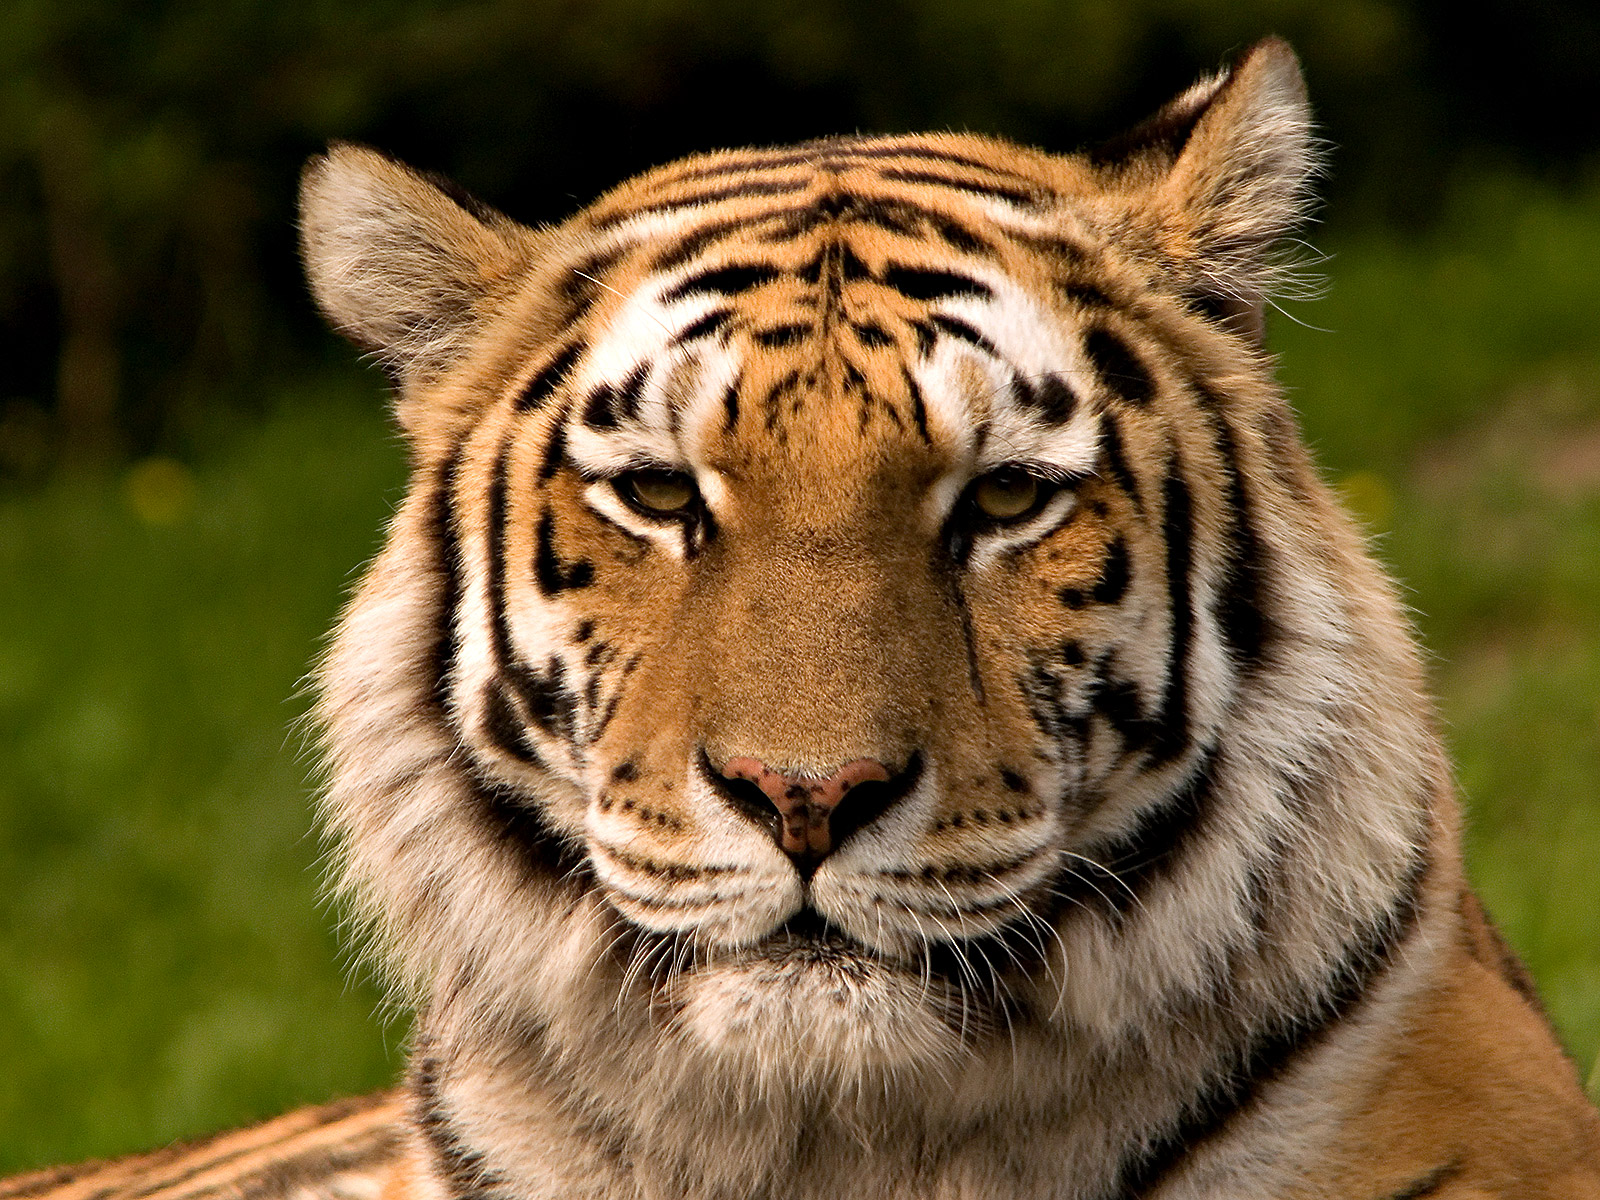
\includegraphics[width=0.5\textwidth]{fig/tiger.jpeg}
    \caption{\label{fig:tiger}A picture of a tiger.}
\end{figure}

Figure~\ref{fig:tiger} is a picture of a tiger.


%==========================================================================================
\subsection{Table}
\label{ss:Table}

\href{http://en.wikibooks.org/wiki/LaTeX/Tables}{Table examples on WIKIBOOKS}.

\begin{table}[htpb]\begin{center}
\caption{Table Example 1}
\begin{tabularx}{8cm}{llX}
\hline
Start & End  & Character Block Name \\
\hline
3400  & 4DB5 & CJK Unified Ideographs Extension A \\
4E00  & 9FFF & CJK Unified Ideographs \\
\hline
\end{tabularx}
 \end{center}\end{table}

\begin{table}[htpb]\begin{center}
\caption{Table Example 2}
\begin{tabular}{llr}
\hline
\multicolumn{2}{c}{Item} \\
\cline{1-2}
Animal & Description & Price (\$) \\
\hline
Gnat  & per gram & 13.65 \\
      & each     &  0.01 \\
Gnu   & stuffed  & 92.50 \\
Emu   & stuffed  & 33.33 \\
Armadillo & frozen & 8.99 \\
\hline
\end{tabular}
 \end{center}\end{table}
 
 \begin{table}[htpb]\begin{center}
	\label{t:prefix-table}
	\caption{Table Example 3}
	\renewcommand{\arraystretch}{1.0}
	\begin{tabularx}{300pt}{|c|X| }
		\hline
		\multirow{1}{*}{\textbf{Allocation}} &
		Allocation, Element, Type, Script 
		\\ \hline\hline
		%------------------------------
		\multirow{6}{*}{\textbf{Data Types}} &
        Byte2, Byte3, and Byte4\\ &
        Float2, Float3, Float4\\ &
        Int2, Int3, Int4\\ &
        Long2, Long3, Long4\\ &
        Matrix2f, Matrix3f, Matrix4f\\ &
        Short2, Short3, Short4
        \\ \hline\hline
		%------------------------------
		\multirow{4}{*}{\textbf{Graphics}} &
		Mesh\\&
		ProgramFragment, ProgramRaster\\&
		ProgramStore, ProgramVertex\\&
		RSSurfaceView
		\\ \hline
		%------------------------------
	\end{tabularx}
\end{center}\end{table}

\begin{table}[htpb]\begin{center}
\caption{Table Example 4}
\begin{tabular}{|l|l|l|}
\hline
\multicolumn{3}{|c|}{Team sheet} \\
\hline
Goalkeeper & GK & Paul Robinson \\ \hline
\multirow{4}{*}{Defenders} & LB & Lucus Radebe \\
 & DC & Michael Duberry \\
 & DC & Dominic Matteo \\
 & RB & Didier Domi \\ \hline
\multirow{3}{*}{Midfielders} & MC & David Batty \\
 & MC & Eirik Bakke \\
 & MC & Jody Morris \\ \hline
Forward & FW & Jamie McMaster \\ \hline
\multirow{2}{*}{Strikers} & ST & Alan Smith \\
 & ST & Mark Viduka \\
\hline
\end{tabular}
 \end{center}\end{table}
 
 \begin{table}[htpb]\begin{center}
\caption{Table Example 5}
 \begin{tabular}{l*{6}{c}r}
Team              & P & W & D & L & F  & A & Pts \\
\hline
Manchester United & 6 & 4 & 0 & 2 & 10 & 5 & 12  \\
Celtic            & 6 & 3 & 0 & 3 &  8 & 9 &  9  \\
Benfica           & 6 & 2 & 1 & 3 &  7 & 8 &  7  \\
FC Copenhagen     & 6 & 2 & 1 & 2 &  5 & 8 &  7  \\
\end{tabular}
 \end{center}\end{table}

%==========================================================================================
\subsection{Verb}
\label{ss:VerbUsage}
Let's take a overview on how to type special characters:\\
\verb|<FRAMEWORKS_BASE>/graphics/java/android/renderscript|\\\footnote{Path of <APP\_intermediates>: <ANDROID\_ROOT>/out/target/common/obj/APPS/APPNAME\_intermediates/}
You could also go back to the beginning of the chapter by the \hyperref[c:GetStarted]{\textbf{hyperref}}.

%==========================================================================================
\subsection{Enumeration}
\label{ss:Enumeration}
\begin{enumerate}
\item Enumerated Item1
\item Enumerated Item2
\item Enumerated Item3
\end{enumerate}

%==========================================================================================
\subsection{Code Display}
\label{ss:CodeDisplay}

\lstset{
	language=C++,
	stringstyle=\rmfamily,
	commentstyle=\itshape\color[rgb]{0.133,0.545,0.133},
	showstringspaces=false,
	basicstyle=\ttfamily\scriptsize,
	numberstyle=\tiny,
	numbers=left,
	stepnumber=1,
	numbersep=10pt,
	tabsize=2,
	breaklines=true,
	prebreak = \raisebox{0ex}[0ex][0ex]{\ensuremath{\hookleftarrow}},
	breakatwhitespace=false,
  	columns=fixed,
  	upquote=true,
  	extendedchars=true,
	xleftmargin=2em,
	xrightmargin=.5em,
	escapeinside={(*@}{@*)},
    mathescape=false,
}
Here is a "Hello, DanDing." example:
\begin{lstlisting}[style=nonumbers] 
void main(int argc, char **argv)
{
    printf("   ˊ_> ˋ  ");
}
\end{lstlisting}


Another example with line numbers:
\begin{lstlisting}
void main(int argc, char **argv)
{
    printf("   ˊ_> ˋ  ");
}
\end{lstlisting}

Matlab example:

\definecolor{dkgreen}{rgb}{0,0.6,0}
\definecolor{gray}{rgb}{0.5,0.5,0.5}
\lstset{language=Matlab,
   keywords={break,case,catch,continue,else,elseif,end,for,function,
      global,if,otherwise,persistent,return,switch,try,while},
   basicstyle=\ttfamily,
   keywordstyle=\color{blue},
   commentstyle=\color{red},
   stringstyle=\color{dkgreen},
   numbers=left,
   numberstyle=\tiny\color{gray},
   stepnumber=1,
   numbersep=10pt,
   backgroundcolor=\color{white},
   tabsize=4,
   showspaces=false,
   showstringspaces=false}

\begin{lstlisting}
function y = demo(x) % This is a comment.
   str = 'hello there';
   y = x + 1;
end
\end{lstlisting}

%==========================================================================================
\subsection{Math}
\label{ss:Math}
\begin{itemize}
    \item Inline mode:\\
The solution to $\sqrt{x} = 5$ is $x=25$.
    \item Display mode:\\
The solution to \[\sqrt{x} = 5\] is \[x=25.\]
    \item Numbered mode:
\begin{equation}
2+2=4
\end{equation}
    \item Non-numbered:
\begin{equation*}
2+2=4
\end{equation*}
    \item Aligning:
\begin{align*}
2x^2 + 3(x-1)(x-2) & = 2x^2 + 3(x^2-3x+2)\\
&= 2x^2 + 3x^2 - 9x + 6\\
&= 5x^2 - 9x + 6
\end{align*}
     \item Fractions:
\[
 \frac{n!}{k!(n-k)!} = \binom{n}{k}
\]
    \item Matrix:
\[
 A_{m,n} =
 \begin{pmatrix}
  a_{1,1} & a_{1,2} & \cdots & a_{1,n} \\
  a_{2,1} & a_{2,2} & \cdots & a_{2,n} \\
  \vdots  & \vdots  & \ddots & \vdots  \\
  a_{m,1} & a_{m,2} & \cdots & a_{m,n}
 \end{pmatrix}
\]
\end{itemize}
\href{http://en.wikibooks.org/wiki/LaTeX/Mathematics}{More examples on WIKIBOOKS}.


%==========================================================================================
\subsection{Algorithms}
\label{ss:Algorithms}
\begin{algorithm}[h]                      % enter the algorithm environment
\caption{Calculate $y = x^n$}          % give the algorithm a caption
\label{alg1}                           % and a label for \ref{} commands later in the document
\begin{algorithmic}                    % enter the algorithmic environment
    \Require $n \geq 0 \vee x \neq 0$
    \Ensure $y = x^n$
    \State $y \Leftarrow 1$
    \If{$n < 0$}
        \State $X \Leftarrow 1 / x$
        \State $N \Leftarrow -n$
    \Else
        \State $X \Leftarrow x$
        \State $N \Leftarrow n$
    \EndIf
    \While{$N \neq 0$}
        \If{$N$ is even}
            \State $X \Leftarrow X \times X$
            \State $N \Leftarrow N / 2$
        \Else[$N$ is odd]
            \State $y \Leftarrow y \times X$
            \State $N \Leftarrow N - 1$
        \EndIf
    \EndWhile
\end{algorithmic}
\end{algorithm}
\href{http://en.wikibooks.org/wiki/LaTeX/Algorithms_and_Pseudocode}{More examples on WIKIBOOKS}.


%\chapter{Introduction}
\label{c:intro}

HiHi Iam r44~. The organization of this thesis is as follows. In chapte~\ref{c:thm}, the theoretical background and definition of surface plasmon will be included~\cite{maier2007plasmonics}. Chapte~\ref{c:exp} contains description of experiment methods such as atomic force microscopy and scanning electron microscopy. 


% Motivation

% Scenario

% Weakness of LeeWave.

% Contribution

\section{Thesis Overview}
\label{s:ThesisOverview}
In this section, we describe the overview of this thesis.

%\bibliographystyle{unsrt}
%\bibliography{thesisbib}
%\chapter{Related Works}
\label{c:related}

%Overall

%CP

%PRP

%LeeWave
Now let's talk about the state-of-the-art method, LeeWave, which is the starting point of our framework. The spirit of LeeWave is to iteratively pruning impossible candidaites until only $k$ instances left by transforming a raw feature vector into an error tree like TODO with the help of the Haar wavelet transformation. Although the total number of coefficients in an error tree would be equal to length of the raw feature vector, the coefficients at the upper levels would be more important than those in the lower levels.  The importance defined here is the chance to contibute more to the final Euclidean distance,  And it could also be observed from the way to calculate the Euclidean distance from the error trees, the higher level the coefficient is, the heavier weight it has to multiply.

Once we have the importance of the coefficients, LeeWave sends coefficents according to their levels in the error tree transformed from the query $q$, from upside to down. In each round, LeeWave would send those coefficients in one level of the tree to each candidate machines.  Then, these machines would return some information that allows the server to compute the bounds between $q$ and the instances in these machines.  With the help of these bounds, the server could prune some instances that they are impossible to be the final answers.  If there are exactly $k$ instances left after pruning, then we just achive our goal to find the $k$NN/$k$FN.  Otherwise, the server would send the next level and repeat the pruning process until finding the answers or sending every level of this tree.
%MsWave

%\bibliographystyle{unsrt}
%\bibliography{thesisbib}
%\input{Method}
%\newcommand{\decision}{\operatornamewithlimits{\gtrless}}
\newcommand{\argmax}{\operatornamewithlimits{argmax}}
\newcommand{\argmin}{\operatornamewithlimits{argmin}}

\chapter{Quantity modulation}
\label{c:qm}

\section{Introduction}
 In this chapter, we study the communication between two nano-machines with information embedded in different molecular quantity~\cite{Andrew1}. In the rest of this chapter, we call this kind of modulation as quantity modulation (QM). It is known that in diffusion-based molecular communications, molecules are emitted by the transmitter and move towards the receiver following the laws of molecule diffusion. Recent studies on diffusion-based molecular communications often model the statistical behavior of molecule diffusion as a Brownian motion~\cite{brown}. Due to the random nature of Brownian motions, molecules that released earlier by TN may arrive late. Therefore, messages carried in current molecules may be interfered by those delayed molecules that were transmitted earlier. 
This phenomenon is known as the ISI effect in diffusion-based molecular communications. A brief discussion about this effect can be found in~\cite{ISI_concen} and~\cite{delaySelector}.

There are lots of ways to design filters to eliminate the effect of ISI in conventional communication such as linear equalizer, adaptive equalizer and decision-feedback equalizer~\cite{commSysEng}. However, both linear equalizer and adaptive equalizer do not work well in molecular communication due to time-varying channel response.
 In this chapter, we utilize the concept of decision feedback and introduce a method to mitigate the effect of ISI.

The rest of this chapter is organized as follows: In Section II, we introduce the settings of a binary QM molecular communication system in details. We also describe the characteristics and the mathematical model of a Brownian motion channel. Section III focuses on deriving the decision rule for one-shot transmission of the binary QM system and extending it to the M-ary transmission case. In Section IV, we consider serial transmission and take ISI effect into account. ISI cancellation method is also described in this section. Numerical results are shown in Section V. Finally, we make conclusions in Section VI.

\section{System model}
In this section, we first give a general model for transmitter, receiver, and channel in molecular communication. We then describe a QM system of $M$ quantity levels ($M$-ary modulation) bearing $\log_2M$ information bits, which will be used later to apply our ISI cancellation method.

\subsection{Transmitter}
Fig.~\ref{fig:machine} illustrates a transmitter nano-machine TN transmitting molecules to a receiver nano-machine RN. When TN receives the information (e.g. bit pattern) to be transmitted, it starts storing certain number of molecules in a vesicle (i.e. container that stores molecules) and release these molecules simultaneously into the environment. The number of released molecules differs according to the transmitting information. In practical situations, molecules leaves the vesicle with random timing which is discussed in~\cite{secrete_phy}. In this paper, we simply assume that molecules exit the vesicle simultaneously.

\begin{figure}[htb]
\centering
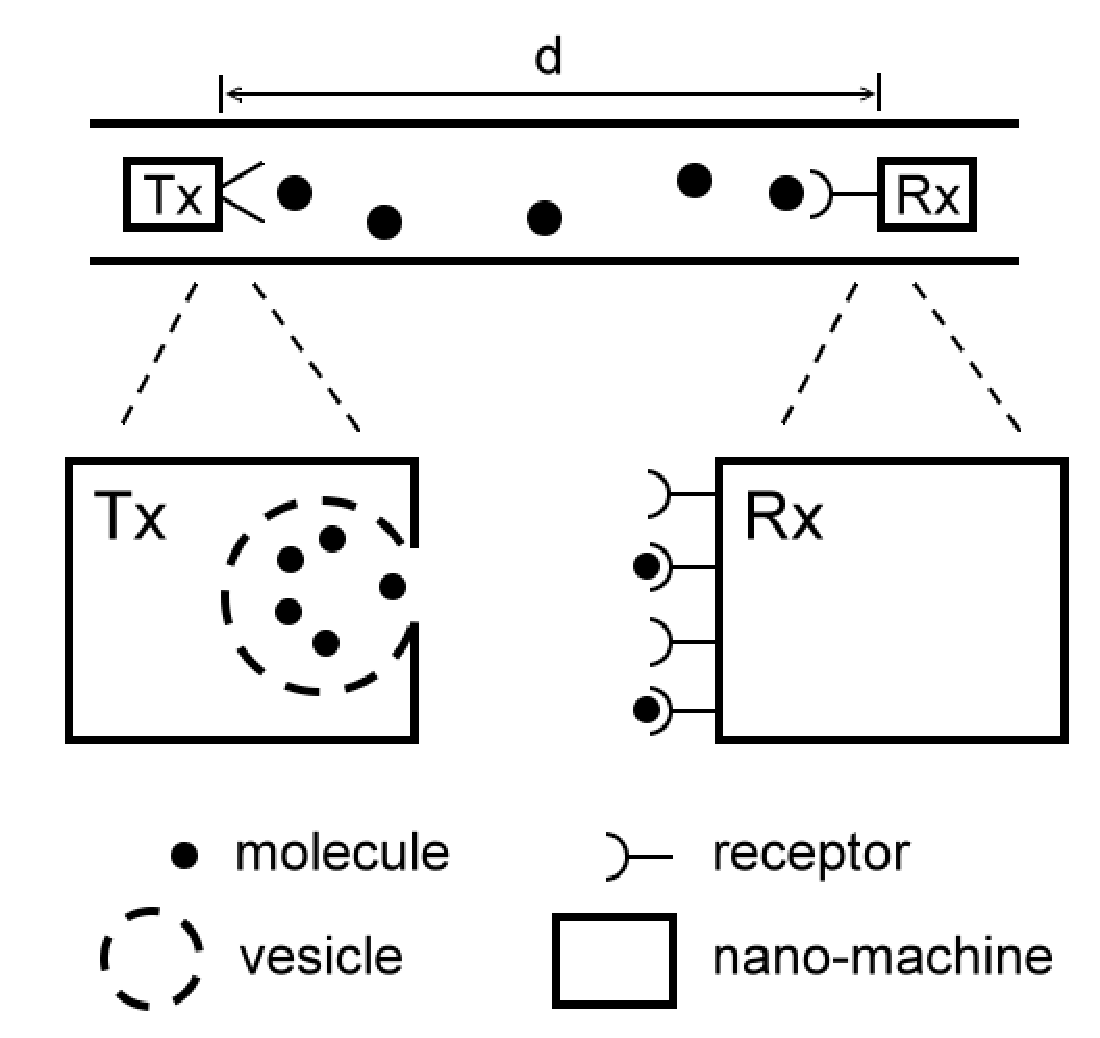
\includegraphics[width=3.5in, keepaspectratio]{QM/machine.eps}
\caption{Transmission from TN to RN through a fluid medium.} \label{fig:machine}
\end{figure}

\subsection{Receiver}
RN is located at a position $d > 0$ apart from TN. There are several receptors capturing molecules on RN. RN counts the number of molecules it captures and perform detection according to the number. We assume the molecules can be perfectly captured by the receptors and RN does not have counting errors. Furthermore, once a molecule arrives at RN, it will be removed from the communication medium.

\subsection{Channel}
Consider a fluid medium between TN and RN with positive drift velocity $v$. The molecules are all constrained to move in a one-dimensional space. We assume that the trajectory of emitted molecules can be modeled with independent Brownian motions\cite{brown}.
Let $X$ denote the random variable representing the first hitting time (i.e. time difference between releasing and capturing) of a molecule. If $v > 0$, it can be shown that the probability density function (pdf) of $X$ is given by the inverse Gaussian (IG) distribution \cite{Chhikara:1989:IGD:73944}

\begin{eqnarray}
f_X(x) = \left\{\begin{array}{ll}
                 \sqrt{\dfrac{\lambda}{2\pi x^3}}\exp \left\{ -\dfrac{\lambda (x-\mu)^2}{2\mu^2 x} \right\}, & \mbox{$x>0$,}
                 \\
                 0, & \mbox{$x \leq 0$,}
                \end{array} \right. \label{IG_PDF}
\end{eqnarray}
\begin{eqnarray}
\mu = \dfrac{d}{v}\text{\ and\ } \lambda = \dfrac{d^2}{2D},\nonumber
\end{eqnarray}
where $D$ denotes the diffusion coefficient which is given by
\begin{eqnarray}
D = \dfrac{k_BT}{6\pi n r} \nonumber
\end{eqnarray}
where $k_B$ is the Boltzmann constant, $T$ is the temperature, $n$ is the viscosity of the fluid medium, and $r$ is the radius of molecule. For simplicity,
 we assume that the radii for all molecules are the same so that the diffusion coefficients are the same.

\subsection{QM system}
 Consider a time-slotted $M$-ary communication with signaling interval $T_s$, TN can release $M$ different quantities of molecules into the channel. Denote those $M$ quantities by $L_m$, where $m \in \{ 0,1,2,\cdots ,(M-1)\}$. Assume the \emph{a priori} probability for releasing $L_m$ molecules to be $q_m$. At the starting time of each transmission time slot, $L_m$ molecules are emitted simultaneously from the transmitter to indicate the transmission of a symbol. We assume perfect synchronization between the transmitter and the receiver. During each time slot, RN counts the total number of arriving molecules. An appropriate decision rule, proposed in Section~\ref{sec_detection}, is then applied to determine the transmitted data bit at the end of each time slot. The molecules which fail to arrive within the corresponding time slot become a source of interference, which will cause performance degradation to the detections of later coming symbols. Fig.~\ref{fig:modulation} is an example of QM system with $M=4$ and uniform quantity levels.

Perfect synchronization between TN and RN is assumed in this chapter, in chapter [ ] we provide a possible realization which is based on sending training molecular impulses and detecting the concentration peaks.

\begin{figure}[htb]
\centering
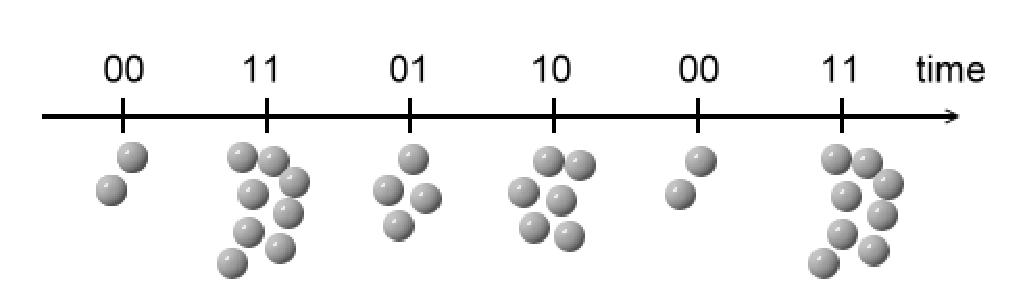
\includegraphics[width=5.5in, keepaspectratio]{QM/modulation.eps}
\caption{Illustration of quantity-based modulation scheme with $L_0=2$, $L_1=4$, $L_2=6$, $L_3=8$.} \label{fig:modulation}
\end{figure}

\section{Detection in one-shot transmission}
In this section, we discuss the detection rule of the system for one-shot transmission. The main contribution of our work is that we separate the ISI cancellation problem from the detection to achieve a more flexible and modularized design, which is different from previous works \cite{ICC_Meng}.

\subsection{Binary Detection}
 We define two hypotheses $H_0$ and $H_1$. $H_0$ is the hypothesis that $L_0$ molecules are transmitted (indicating bit $0$), and $H_1$ is the hypothesis that $L_1$ molecules are transmitted
 (indicating bit $1$).
 Denote the conditional pdf of the number of received molecules in a particular time slot, given that hypothesis $H_m$ is true, by $P(N=n | H_m)$, $m\in\{0,1\}$.
Using the inverse Gaussian pdf given in~\eqref{IG_PDF}, we define
the probabilities $p_j$ as:
\begin{eqnarray}
p_j = \int^{(j+1)T_s}_{j Ts} f_X(x)dx
\end{eqnarray}
for $j\in \{0,1,\cdots\}$, which is the probability that the traveling time of a molecule falls in the interval $[j T_s,(j+1)T_s]$,
where $j$ is the index of the time slots.
Define $Y_k$ to be the indicator random variable showing whether the $k$-th molecule emitted in a one-shot transmission arrives within $T_s$ given that $H_m$ is true. That is,
\begin{eqnarray}
Y_k = \left\{\begin{array}{ll}
                 1, & \mbox{if the $k$-th molecule arrives within $T_s$,} \\
                 \\
                 0, & \mbox{otherwise.} \\
                \end{array} \right.
\end{eqnarray}
Let $N$ be the random variable denoting the total number of molecules arriving at the receiver within a particular time slot. We have the following relation:
\begin{eqnarray}
P(N=n| H_m)=P(Y_1+Y_2+...+Y_{L_m}=n).
\end{eqnarray}
Given the number of the transmitted molecules, $N$ thus follows a binomial distribution with mean and variance as $L_m p_0$ and $L_m p_0(1-p_0)$, respectively. For large $L_m$, we approximate the binomial distribution by a Gaussian distribution with the knowledge of the mean and variance of $N$. Since it is difficult to manipulate directly with the binomial pdf, we will derive our detection threshold using Gaussian approximations instead.
Namely, we have
\begin{eqnarray}
P(N=n| H_m) \approx \dfrac{\exp
\left\{-\dfrac{(n-L_m p_0)^2}{2 L_m p_0(1-p_0)}\right\}}{\sqrt{2\pi L_m p_0(1-p_0)}}.
\end{eqnarray}
As a special case, the distributions of $N$ under two hypotheses can thus be obtained as
\begin{eqnarray}
P(N=n| H_0) \approx \dfrac{\exp\left\{-\dfrac{(n-L_0p_0)^2}{2L_0p_0(1-p_0)}\right\}}{\sqrt{2\pi L_0p_0(1-p_0)}}, \label{eq:h0}
\end{eqnarray}
\begin{eqnarray}
P(N=n| H_1) \approx \dfrac{\exp\left\{-\dfrac{(n-L_1p_0)^2}{2L_1p_0(1-p_0)}\right\}}{\sqrt{2\pi L_1p_0(1-p_0)}}. \label{eq:h1}
\end{eqnarray}
According to the conventional hypothesis testing theory \cite{vanTree, poor},
the decision rule can be expressed using the likelihood ratio $\Lambda(N)$ as
\begin{eqnarray}
\Lambda(N) =  \dfrac{P(N| H_1)}{P(N| H_0)} \decision ^{H_1}_{H_0} \dfrac{q_0}{q_1}.
\end{eqnarray}
If we assume equal \emph{a priori} probabilities $q_0=q_1=1/2$, due to the characteristic of Gaussian distribution shown in Fig.~\ref{fig:gaussian},  the decision rule can be further reduced to
\begin{eqnarray}
N \decision ^{H_1}_{H_0} \eta
\end{eqnarray}
for some threshold $\eta$,
where $\eta$ is the solution of the following equation:
\begin{eqnarray}
P(N = \eta | H_0) = P(N = \eta | H_1).
\end{eqnarray}
By~\eqref{eq:h0} and~\eqref{eq:h1}, we have
\begin{eqnarray}
\sqrt{ \dfrac{L_1}{L_0} } = \exp \left\{  \dfrac{(L_1-L_0) (\eta^2 - p_0^2L_0L_1) }{2 L_0 L_1 p_0(1-p_0)} \right\}.
\end{eqnarray}
Taking logarithms to both sides, the equation becomes
\begin{eqnarray}
\eta = \sqrt{ \dfrac{ L_1L_0\ln (L_1/L_0) }{L_1-L_0}p_0(1-p_0)+p_0^2L_0L_1 }. \label{eq:threshold}
\end{eqnarray}
In other words, if the received number of molecules is greater than the threshold $\eta$,  the receiver will determine $H_1$ as the hypothesis testing result; otherwise $H_0$ will be decided.

\begin{figure}[htb]
\centering
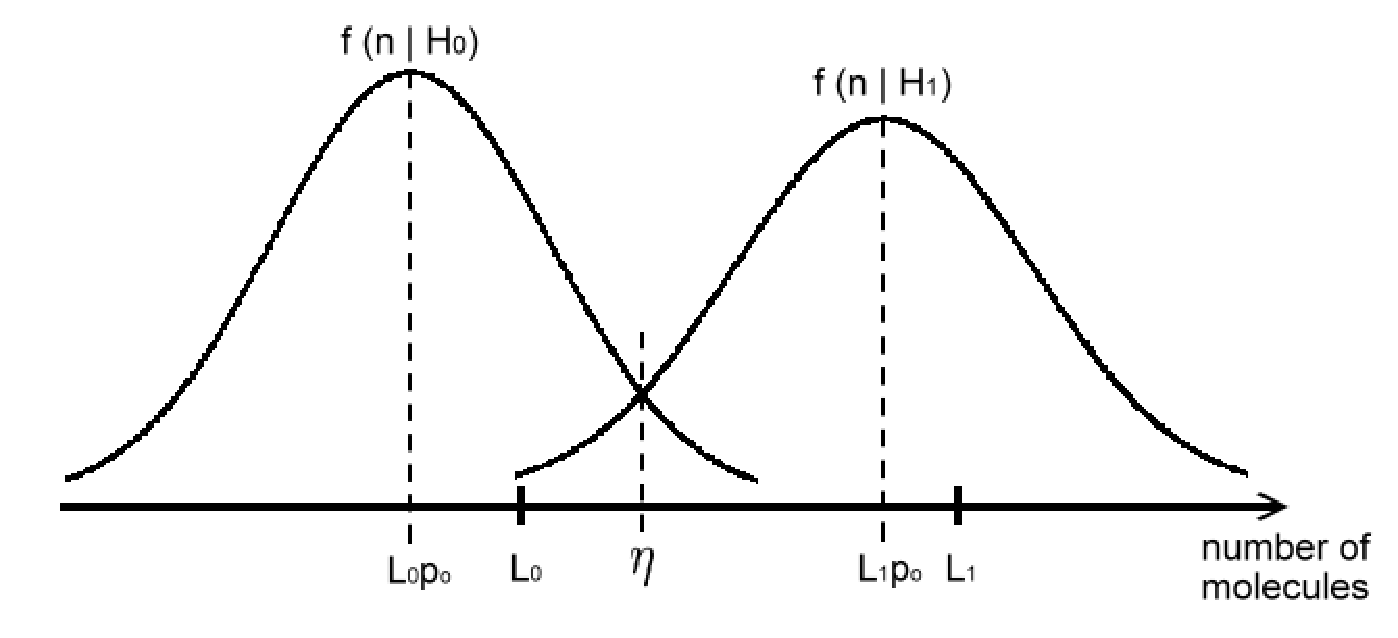
\includegraphics[width=5.5in, keepaspectratio]{QM/gaussian.eps}
\caption{Demonstration of the process of finding $\eta$ in a binary QM system, where $f$ is the conditional pdf of $N$ given $H_m$ is true.} \label{fig:gaussian}
\end{figure}

\subsection{M-ary Detection}
The detection rule can be extended to $M$-ary detection with only a few adjustments.
Suppose we have multiple hypotheses $H_m$ where $m \in \{ 0,1,2,\cdots,(M-1) \}$ which represent the transmission of $L_m$ molecules.
The goal is to decide which $\hat{m}$ we should choose.
The maximum \emph{a priori} (MAP)
detection rule is:
\begin{eqnarray}
\hat{m}(N) = \argmax_{m}P(N | H_m).
\end{eqnarray}
Due to the properties of Gaussian distribution, the above MAP detection rule can be simplified to pairwise comparisons between the ``neighboring'' conditional probability distributions.

To write down the expressions explicitly, we define a set of thresholds
$E = \{\eta_j \in [-\infty,\infty]\ :\ j = 0,1,2,\cdots,M \}$, and let $\eta_0 = -\infty$ and $\eta_M = \infty$.
For $j=1,2,\cdots,(M-1)$, $\eta_j$ can be obtained by solving the equations
\begin{eqnarray}
P(N=\eta_j | H_{j-1}) = P(N=\eta_j | H_j).
\end{eqnarray}
With the thresholds determined, the detection rule for $M$-ary transmission can be
expressed as
\begin{eqnarray}
\hat{m}(N) = \sum^{M-1}_{k=0}k \cdot u\left[-(N-\eta_k)(N-\eta_{k+1})\right].
\end{eqnarray}
where $u(\cdot)$ denotes the unit step function.

\subsection{Error Rate Analysis}
After the construction of the transmission and decision rules, we then analyze how it performs in terms of symbol or bit error rate. Consider a specific case for $M=2$ and $q_0 = q_1 = 1/2$. Denote the false alarm probability as $P_F$ and the missing probability as $P_M$. The error rate can be written as
\begin{eqnarray}
P_e = q_0P_F+q_1P_M=\dfrac{1}{2}(P_F+P_M). \label{eq:error}
\end{eqnarray}
From Fig.~\ref{fig:gaussian} and the decision rule derived in Subsection A, it can be shown that
\begin{eqnarray}
P_F = P(N>\eta | H_0) = Q\left( \dfrac{\eta-L_0p_0}{\sqrt{L_0 p_0 (1 - p_0)}} \right), \label{eq:falseAlarm}
\end{eqnarray}
\begin{eqnarray}
P_M = P(N < \eta | H_1) = Q\left( \dfrac{L_1p_0 - \eta}{\sqrt{ L_1 p_0 (1 - p_0)}} \right), \label{eq:missing}
\end{eqnarray}
where $Q(\cdot)$ denotes the Q-function.
By substituting~\eqref{eq:threshold} into equation~\eqref{eq:falseAlarm} and~\eqref{eq:missing}, we can evaluate the
error rate $P_e$ in~\eqref{eq:error}. Fig.~\ref{fig:error_rate} shows the comparison between our analysis and numerical results.

\begin{figure}[htb]
\centering
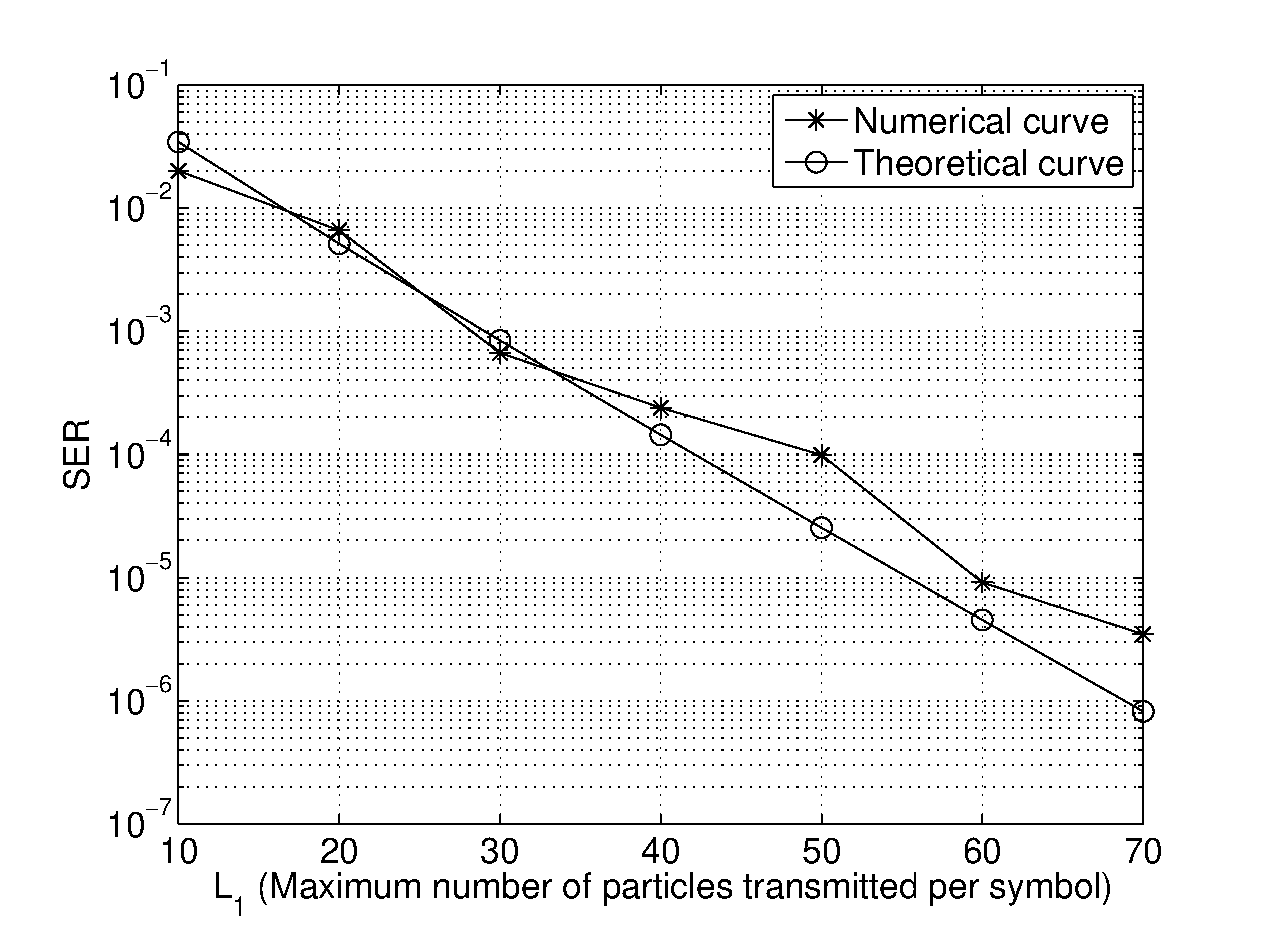
\includegraphics[width=5.5in, keepaspectratio]{QM/analysis_0329.eps}
\caption{Theoretical result versus numerical result for one-shot binary quantity-based modulation.} \label{fig:error_rate}
\end{figure}

\section{Serial transmision and ISI cancellation}
The above described QM molecular communication system seems to work already. However, in practical situations, we need to perform serial transmissions rather than one-shot transmission. Thus the ISI effect must be taken into account.
Our results show that if we do not modify our one-shot detection rule, the system performance will fall dramatically under serial transmission environments due to the severe ISI effect. To solve this problem, we propose a method to mitigate the ISI effect.

In order to mitigate the ISI effect, we first need an estimation of the number of the delayed molecules that come from former time slots. If we know the conditional probability distribution of the number of ISI molecules conditioned on the current received number, then we can estimate the ISI effect as the conditional mean.
However, the conditional distribution does not have a closed-form solution for inverse Gaussian random variables. Here we proposed another intuitive way to do this estimation.

First, we define ``memory-$\Gamma$ cancellation'' to mean that the ISI effect during the past $\Gamma$ time slots are taken into account when making decision. We first use memory-$1$ cancellation as a demonstrative example.
Suppose that the traveling time $\tau$ of each molecule can be described using an inverse Gaussian random variable with cumulative distribution function (cdf) $F_{\tau}(t)=\int_0^t f_X(x)dx$. Our proposed ISI cancellation method is: if the number of molecules received during the $(i-1)$-th time slot is $n_{i-1}$ and the decided transmission quantity level is $\hat{l}_{i-1}$, where $\hat{l}_{i-1} \in \{ L_0,L_1,\cdots,L_{M-1} \}$, we then subtract $\hat{l}_{i-1}\cdot[F_{\tau}(2T_s)-F_{\tau}(T_s)]$ (the \emph{a priori} expected received number in the $i$-th time slot from the $(i-1)$-th time slot) from $n_i$ before making the $i$-th decision. In other words, the actual number $\tilde{n}_i$ used in making decision is
\begin{eqnarray}
\tilde{n}_i = n_i - \hat{l}_{i-1}\cdot[F_{\tau}(2T_s)-F_{\tau}(T_s)].
\end{eqnarray}
Likewise, we can perform memory-$\Gamma$ cancellation if we have enough buffer at the receiver end to memorize temporarily the recently received numbers of molecules. More explicitly, denote the probabilities that a single transmitted molecule arrives during the time interval $[ j T_s,(j+1) T_s ]$ by $p_j$ for $j\in \mathbb{N} \cup \{0\}$ as before. If the decided transmission quantity level of the current time slot is $\hat{l}$, where $\hat{l} \in \{ L_0,L_1,\cdots,L_{M-1} \}$, then the received number of molecules $j$ time slots later should be subtracted by
$\hat{l} \cdot p_{j+1}$ before making decision. In other words, if the number of molecules received in $i$-th time slot is $n_i$, the actual number $\tilde{n}_i$ used in making decision is
\begin{eqnarray}
\tilde{n}_i = n_i - \sum^{\Gamma}_{j=1}\hat{l}_{i-j}p_{j+1}.
\end{eqnarray}
For binary QM systems, the decision rule can be written as
\begin{eqnarray}
\tilde{n}_i = n_i - \sum^{\Gamma}_{j=1}\hat{l}_{i-j}p_{j+1} \decision ^{H_1}_{H_0} \eta.
\end{eqnarray}
The extension to M-ary QM systems is straightforward.

\section{Numerical results}
In this section, we first discuss the binary and $M$-ary QM modulation systems with and without performing ISI cancellation.
After that, we make comparisons of the system performance under different time slot durations.

The number of molecules is one of the main resources utilized in molecular communications.
Analogous to the ``power'' concept in conventional communications, we need to take this number into account when comparing the system performances.
In the following subsections, we present the results under different maximum number of molecules allowed per symbol, and the quantity levels are uniformly spaced.
The simulation parameters are $d = 0.2\ cm$, drift velocity $v = 0.01\ cm/s$, diffusion coefficient $D = 0.05\ cm^2/s$ , and time slot duration $T_s = 5\ s$.

\subsection{SER comparison with and without ISI cancellation}
In Fig.~\ref{fig:binary_ser}, a binary transmission system with memory-1 and memory-2 cancellaion is considered. The SER drops from $0.04$ to $0.01$ when $L_1=30$, and drops from $10^{-2}$ to $10^{-4}$ when $L_1 = 90$. The improvement grows as $L_1$ increases, which means that by choosing $L_1$ properly, a reliable end-to-end transmission can be achieved. We also observe that even without ISI cancellation, the error rate will drop as $L_1$ increases. The reason is that the spacing between symbols is increased. However, as shown in Fig.~\ref{fig:4ary_ser}, it is not the case for the quaternary transmission system. It can be seen that even though $L_3$ becomes large, the error rate is still high without ISI cancellation, which means we cannot rely solely on increasing the maximum number of molecules without ISI cancellation.

It is worth mentioning that the ISI cancellation method can be performed not only in such quantity-based modulation systems, but it can also be used in other systems like on-off keying\footnote{Transmitting zero or a single molecule.}
with slight modifications.

\begin{figure}[htb]
\centering
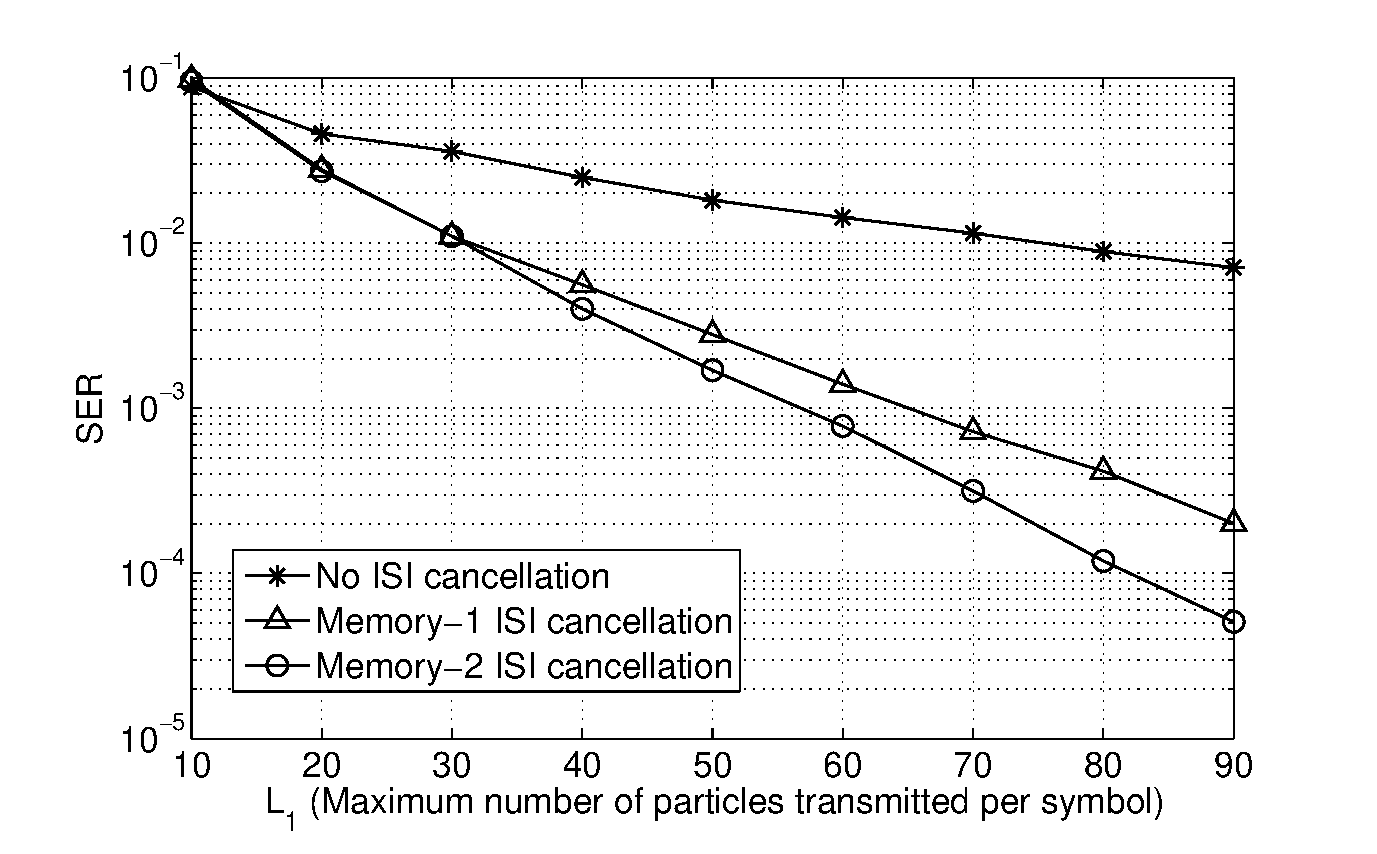
\includegraphics[width=5.5in, keepaspectratio]{QM/binary_ser_0322.eps}
\caption{Binary quantity-based modulation with ISI cancellation.} \label{fig:binary_ser}
\end{figure}

\begin{figure}[htb]
\centering
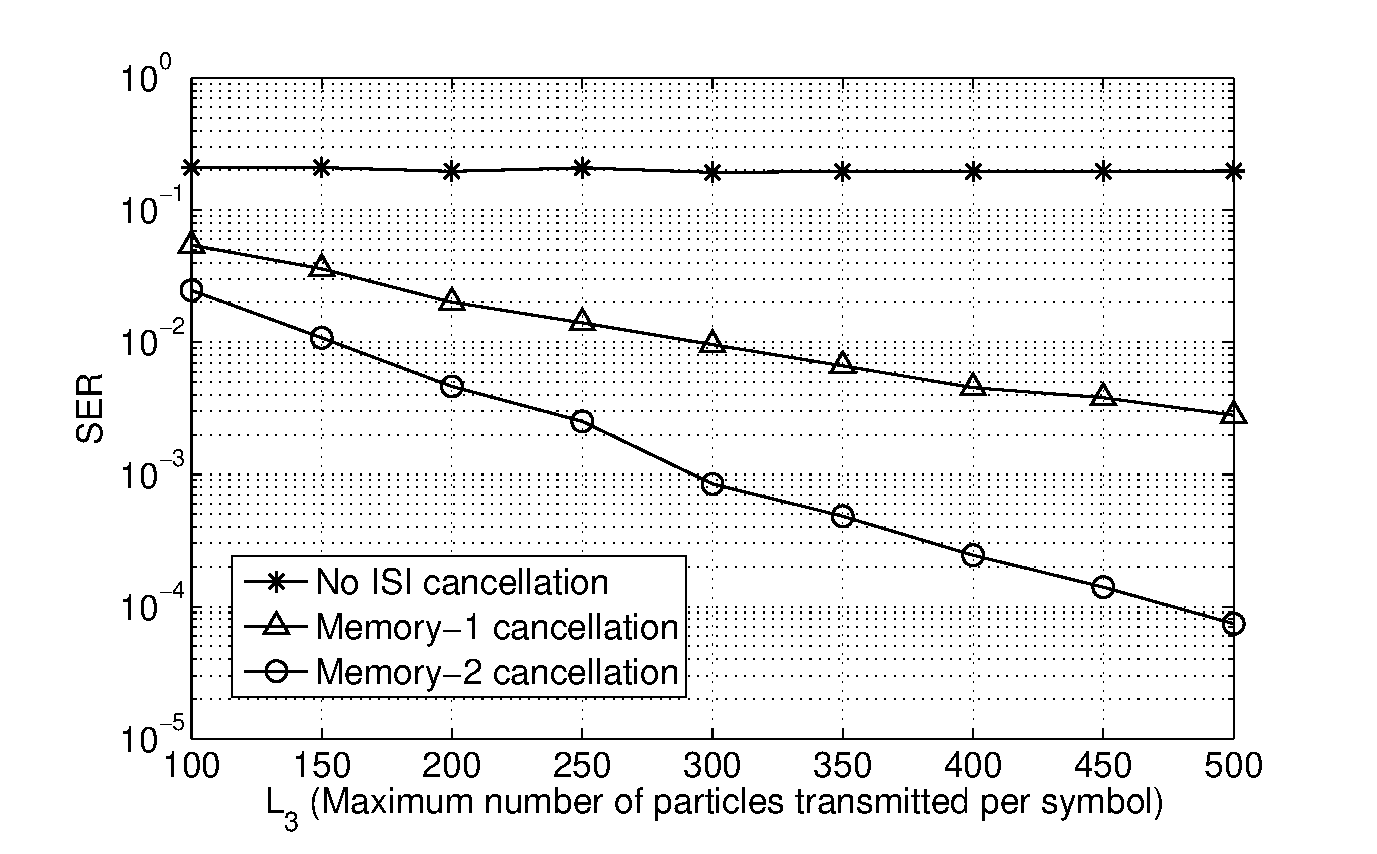
\includegraphics[width=5.5in, keepaspectratio]{QM/4ary_ser_0322.eps}
\caption{Quaternary quantity-based modulation with ISI cancellation.} \label{fig:4ary_ser}
\end{figure}

\subsection{Performance Under Different Duration of Time Slot}
In this subsection, we consider a binary transmission system with and without ISI cancellation for different time slot durations. From Fig.~\ref{fig:timeslots}, we can observe that the SER decreases as the duration $T_s$ increases. In other words, to improve performance, one can increase the duration of the time slot as shown in Fig.~\ref{timeslots}. Although the error rate is already quite acceptable, it can be further improved by the ISI cancellation approach. The improvements is about $10$ times better when $T_s = 10\ s$ and $L_1=70$. Note that when $T_s$ is small, say $T_s = 1\ s$, compared to the expected first-hitting time $d/v$, the error rate increases even if we increase $L_1$ when no cancellation is performed. This is because when $T_s$ is small, molecules tend not to arrive in one symbol time but stay in the background, and that a larger $L_1$ will cause a larger amount of molecules to be in the background and hence larger interference.

\begin{figure}[htb]
\centering
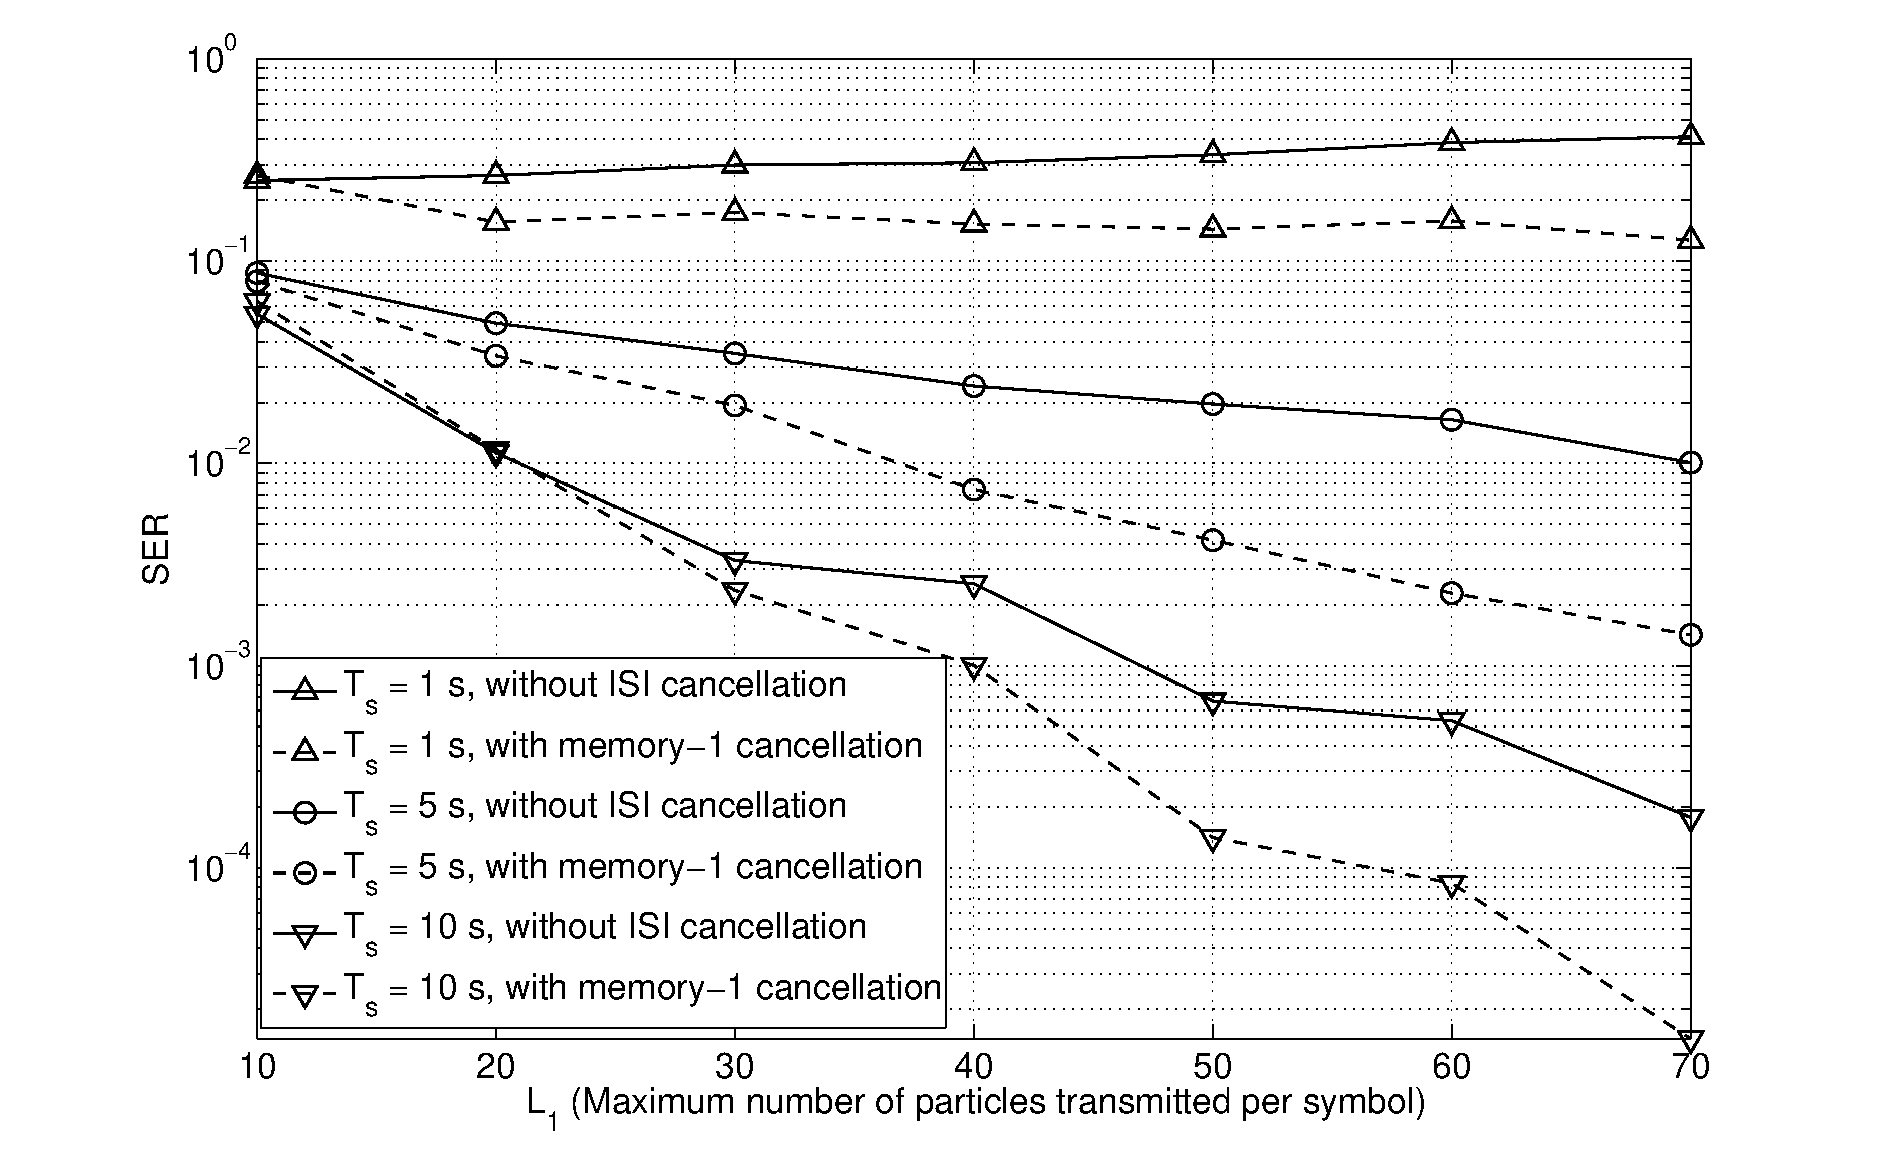
\includegraphics[width=5.5in, keepaspectratio]{QM/timeslots.eps}
\caption{Binary quantity-based modulation with ISI cancellation under different $T_s$.} \label{fig:timeslots}
\end{figure}

%\chapter{Theory of surface plasmon polaritons in metallic nano-structures}
\label{c:thm}
\section{Definition of plasmon}

Plasmon is collective oscillation of conduction electron gas, a quasi-particle resulting from the quantization of plasma oscillations just like phonons are quantizations of mechanical vibrations. The simplest case is the volume plasmon as shown in Figure~\ref{fig:bulk}.
\begin{figure}[htb]
\centering
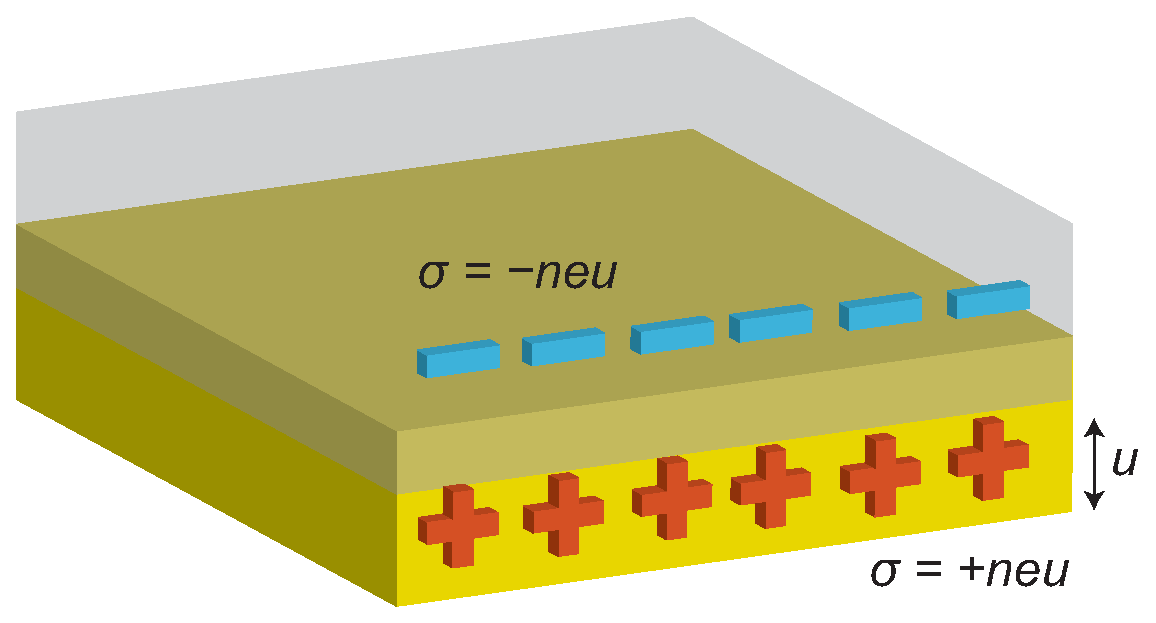
\includegraphics[scale=0.5]{THM/bulk.eps}
\caption{\label{fig:bulk}Longitudinal collective oscillations of the conduction electrons of a metal (Volume plasmons)}
\end{figure}
 We can derive plasma frequency $\omega_p$ from the simple harmonics oscillation model, a collective displacement of the electron cloud by a distance $u$ leads to a surface charge density $\sigma = \pm neu$ at the slab boundaries. This establishes a homogeneous electric field $\mathbf{E} = \frac{neu}{\varepsilon_0}$ inside the slab. Thus, the displaced electrons experience a restoring force, and their movement can be described by the equation of motion $nm\ddot{u} = -ne\mathbf{E}$. Inserting the expression for the electric field, this leads to
 \begin{subequations}
 \begin{align}
 nm\ddot{u} = -\frac{n^2e^2u}{\varepsilon_0} \\
 \ddot{u} + {\omega_p}^{2}u = 0\text{.}
 \end{align}
 \end{subequations}
  The plasma frequency $\omega_p = \sqrt{\frac{ne^2}{\varepsilon_0m}}$ can thus be recognized as the natural frequency of a free oscillation of the electron sea. The quanta of these charge oscillations are called plasmons. Due to the longitudinal nature of the excitation, volume plasmons do not couple to transverse electromagnetic waves, and can only be excited by particle impact. We can derive the dispersion relation of the generalization of volume plasmons, traveling plasma waves, from curl electric field equations (Equations~\ref{eq:curlE})
 \begin{subequations}
 \begin{align}
 \curl{\curl \mathbf{E}} &= -\mu_0 \frac{\partial^2\mathbf{D}}{\partial t^2}\label{eq:curlE}\\
\mathbf{K}( \mathbf{K}\cdot \mathbf{E}-K^{ 2 }\mathbf{E} ) &=-\varepsilon ( \mathbf{K},\omega  ) \frac { { \omega  }^{ 2 } }{ { c }^{ 2 } } \mathbf{E}
 \end{align}
 \end{subequations}  
and plasma model, and a simple equation of motion for an electron of the plasma subjected to an external electric field $\mathbf{E}$
 \begin{equation}
m\ddot{\mathbf{x}} + m\gamma\dot{\mathbf{x}} = -e\mathbf{E}\text{.}
\end{equation}
Assuming a harmonic time dependence $\mathbf{E}( t )=\mathbf{E}_0\mathrm{e}^{-i\omega t}$ of the driving field, a particular solution of this equation describing the oscillation of the electron is $\mathbf{x} ( t ) = \mathbf{x}_0 \mathrm{e}^{-i\omega t} $. The complex amplitude $\mathbf{x}_0$ incorporates any phase shifts between driving field and response via
\begin{equation}
\mathbf{x} ( t ) = \frac{e}{m( \omega^2 + i\gamma\omega )}\mathbf{E}( t )\text{.}
\end{equation}
The displaced electrons contribute to the macroscopic polarization
\begin{equation}
\mathbf{P}=-\frac{ne^2}{m( \omega^2 + i\gamma\omega )}\mathbf{E}( t )\text{.}
\end{equation}
Inserting $\mathbf{P}$ into dielectric displacement field equation $\mathbf{D} = \varepsilon_0\mathbf{E} + \mathbf{P}$ yields
\begin{equation}
\mathbf{D} = \varepsilon_0(1-\frac{\omega_p^2}{\omega^2 + i\gamma\omega})\mathbf{E}\text{,}
\end{equation}
where $\omega_p^2 = \frac{ne^2}{\varepsilon_0m}$. Therefore, the dielectric function of the free electron gas
\begin{equation}
\varepsilon(\omega) = 1- \frac{\omega_p^2}{\omega^2 + i\gamma\omega}\text{.}\label{eq:dielefu}
\end{equation}
We arrive at the desired result by using equation~\ref{eq:dielefu} and the generic dispersion relation $K^2=\varepsilon(\mathbf{K},\omega)\frac{\omega^2}{c^2}$, the dispersion relation of traveling waves becomes
\begin{equation}
\omega^2 = \omega_p^2 + \mathbf{K}^2c^2\text{.}
\end{equation}
From this relation, we can figure out the oscillation properties in any frequency of external field. Note that this branch can not confine the electromagnetic waves, it would radiate out the energy, so this mode is also called radiative surface plasmon.

\section{Surface plasmon polaritons at interface between dielectric and metal}

Surface plasmon polaritons (SPPs) are eigenmodes of transverse magnetic (TM) waves, which coupling the electromagnetic fields to oscillations of the conductor's electron plasma, propagate at a interface between dielectric and metal, and are confined in perpendicular direction. Providing a flat interface between dielectric and metal half-spaces with dielectric constants $\varepsilon_d$ and $\varepsilon_m$ , respectively, and assuming the interface normal to z direction and the SPPs propagate along the $x$ direction, the SPP wave vector $\beta$ is related to the frequency $\omega$ through the dispersion relation
\begin{equation}
\beta = k_0\sqrt{\frac{\varepsilon_d\varepsilon_m}{\varepsilon_d + \varepsilon_m}}\text{,}\label{eq:sppsdisp}
\end{equation}
where $k_0 = \omega/c$ is the free-space wave vector. We take $\omega$ to be real and allow $\beta$ to be complex.

The optical response of metals is often described by the Drude model for a free-electron gas~\cite{kittel1976introduction},
\begin{equation}
\varepsilon_{Drude}(\omega)=1-\frac{\omega_p^2}{\omega^2+i\Gamma\omega}\text{,}
\end{equation}
in which $\Gamma$ is a damping rate due to electron-electron and electron-phonon scattering.
Figure~\ref{fig:SPPdisp} shows the dispersion curve~\ref{eq:sppsdisp} with Drude metal  in the absence of losses ($\Gamma=0$) for air ($\varepsilon_d = 1$) and fused silica ($\varepsilon_d = 2.25$) interface.
\begin{figure}[htb]
\centering
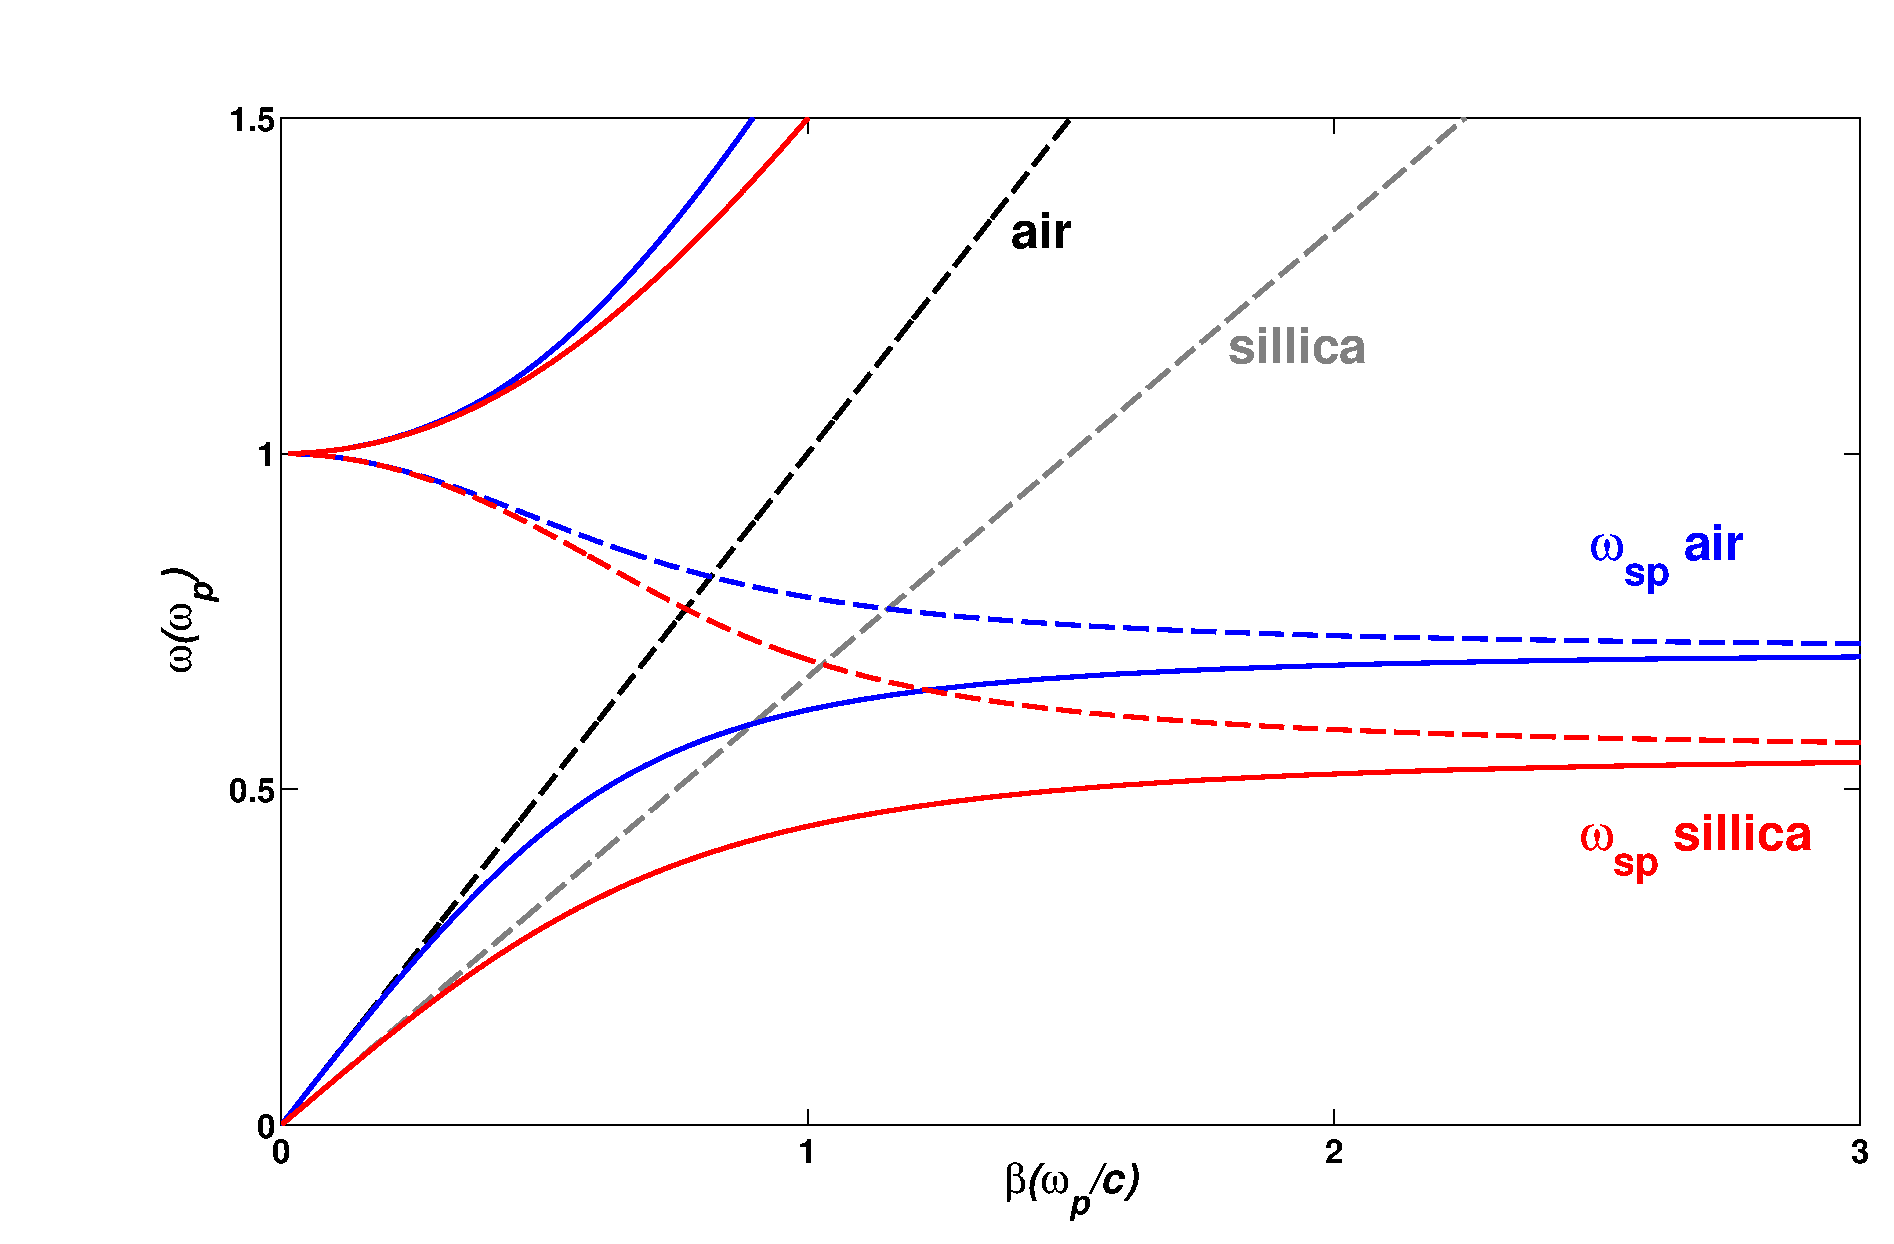
\includegraphics[scale=0.4]{THM/SPPdisp.eps}
\caption{\label{fig:SPPdisp}Dispersion relation of SPPs at the interface between a Drude metal with negligible collision frequency and air (blue curves) and silica (red curves).}
\end{figure}
For small wave vectors SPPs propagation constant $\beta$ is close to $k_0$ at the light line, in the opposite regime of the frequency close to surface plasmon frequency $\omega_p$. It also shows that the SPPs line lying to the right of the respective light lines of air and silica, so that SPPs are directed by light due to phase mismatching. The wave vector mismatch between SPPs and radiation modes needs to be overcome in order to excite or detect SPPs. This can be achieved by multiple methods~\cite{raether1988surface}. In the Otto configuration, light in a prism that is brought in close vicinity to a metal surface can excite SPPs through coupling to the evanescent field. Because light in the prism has a larger wave vector than that in air, it can be phase-matched to the SPPs. In the related Kretschmann-Raether geometry, coupling to SPPs occurs through a metal film that is deposited on a prism. In the grating coupling configuration, metal surface with a shallow grating of grooves or holes with lattice constant $a$. For the simple 1D grating of grooves depicted in Figure~\ref{fig:grating},
\begin{figure}[htb]
\centering
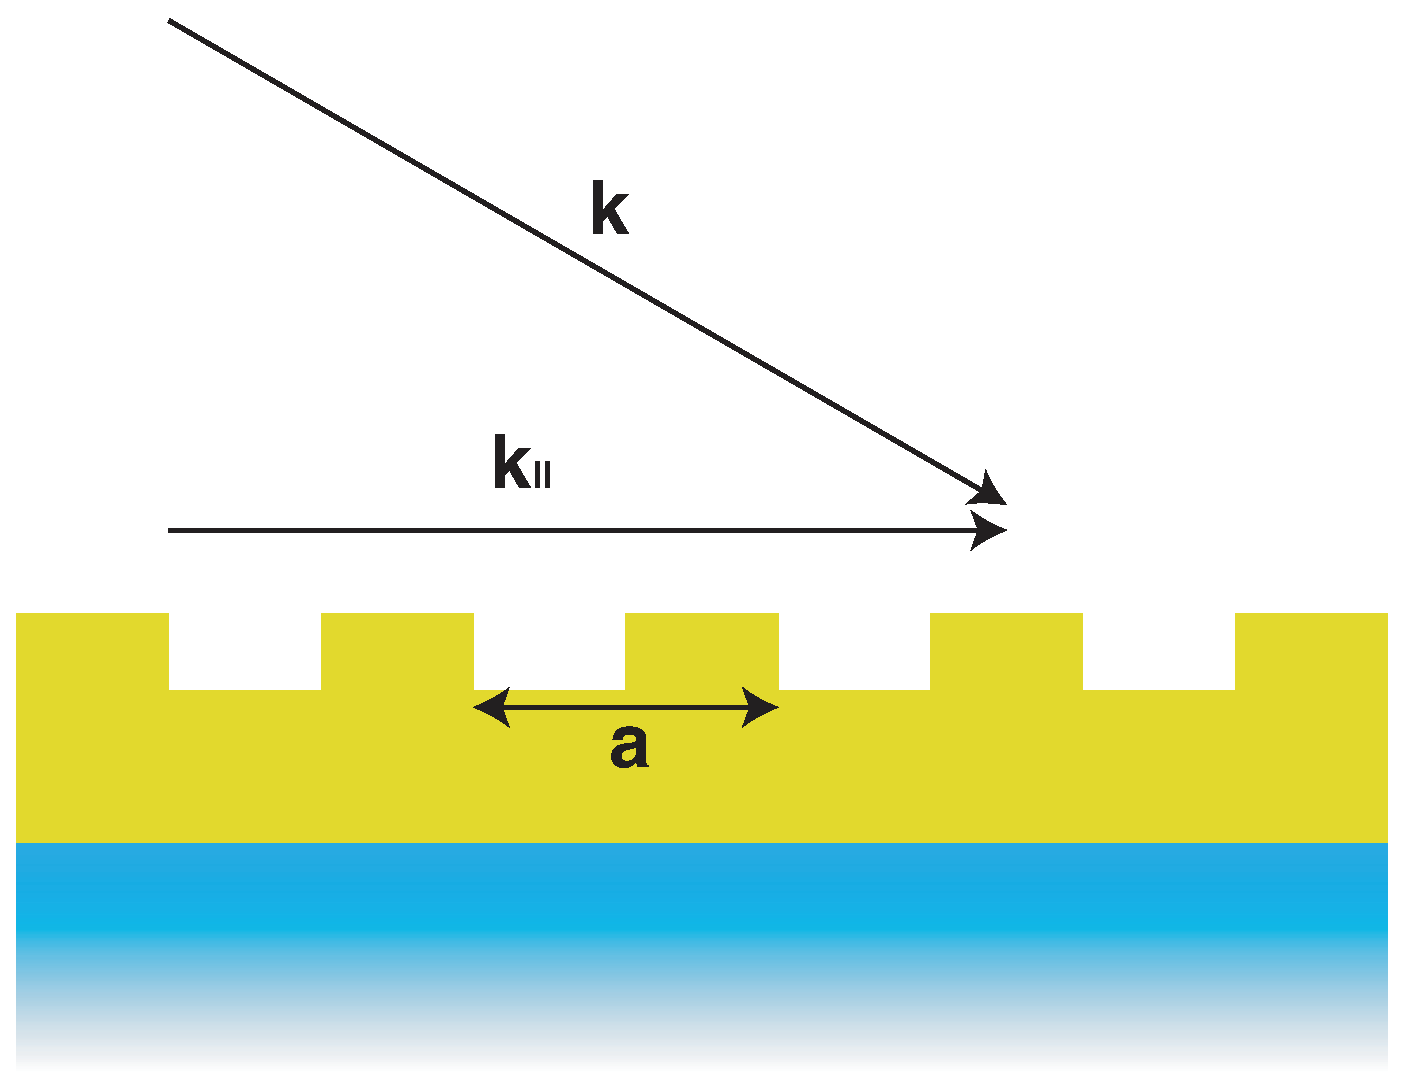
\includegraphics[scale=0.5]{THM/grating.eps}
\caption{\label{fig:grating}Phase-matching of light to SPPs the grating coupling configuration.}
\end{figure}
phase-matching takes place when the condition is fulfilled
\begin{equation}
\beta = k_0 \sin{\theta} \pm \nu g\text{,}
\end{equation}
where $g=\frac{2\pi}{a}$ is the reciprocal vector of the grating, and $\nu=(1,2,3\dots)$.
As with prism coupling, excitation of SPPs is detected as a minimum in the reflected light. The reverse process can also take place, SPPs propagating along a surface modulated with a grating can couple to light and thus radiate. 

%\bibliographystyle{unsrt}
%\bibliography{thesisbib}
%\chapter{Experiment}
\label{c:exp}

\section{Experiment Setup} % (fold)
\label{s:experiment_setup}

In this section, we discuss the resluts of our experiments.  There are four parts in our experiments.  First, we compare our framework with other frameworks in the communication cost.  Second, since there are several stages of improvement in our framework, we discuss each of their influence to our final model.  Third, we consider the amortization of transmitting the orthogonal matrices.  Finally, we compare the power of pruning among different bounds.  For every experiment, we collect the results of $100$ experiments by randomly picking our $100$ instances as the queries.
% section experiment_setup (end)

\section{Data Description} % (fold)
\label{s:data_description}

The table \ref{table:datasets} is the description of those datasets we used in our experiments. Note that the $n\times m$ in the final column means that there are $n$ instances placed in each machine and $m$ machines used in this experiments.  For instance, for the image dataset ANN with SIFT feature, there are totally $5000$ machines and each has $200$ instances in our experiments.

\begin{table}[htpb]\begin{center}
\caption{Summary for each dataset}\label{table:datasets}
\begin{tabular}{|c|c|c|c|c|}
\hline 
Type & Dataset & Feature & Num of Dimensions & Num of Instances\\ \hline \hline
Time Series & Random Walk & $N(0,1)$ & 128 & $200\times 5000$\\ \hline
\multirow{3}{*}{Image} & ANN & SIFT & 128 & $200\times 5000$\\ 
\cline{2-5}
 & \multirow{2}{*}{Flickr} & CSD & 256 & $500\times 2000$\\ 
\cline{3-5}
 & & SCD & 256 & $500\times 2000$\\ \hline
 \multirow{2}{*}{Audio} & \multirow{2}{*}{Million Songs} & MVD & 480 & $500\times 1900$ \\ 
 \cline{3-5}
 & & TRH & 480 & $500\times 1900$\\ \hline
\end{tabular}
\end{center}\end{table}

\subsection{Time Series Data} % (fold)
\label{ssb:time}
The time series datasets we used is a synthetic dataset.  We use the random walk data model in \cite{time}.  Each time series is generated by a random walk whose every step size is a normal distributed random number with mean $0$ and standard deviation $1$.  We also use this model to generate the synthetic dataset in the experiments of MsWave \cite{MsWave}.
% subsection time (end)

\subsection{Image Data} % (fold)
\label{ss:Image}
We use two datasets in our experiments for images.  First is the data provied in \cite{ANN}, which is a widely used dataset for evaluate the performance of approximate nearest neighbors search algorithms.  The another one is the Flickr datasets with two kind of features used in \cite{Flickr}.  The dataset is also a widely used dataset in the task of image retrieval.  The CSD indicates \emph{Color Structure Descriptor} while the SCD means \emph{Scalable Color Descriptor}.
% subsection Image (end)

\subsection{Audio Data} % (fold)
\label{sub:audio_data}
Here we use the audio data named Million Song Dataset from~\cite{Bertin-Mahieux2011} which is a free-available collection of audio features for a million contemporary popular music tracks. For the features, MVD means \emph{Modulation Frequency Variance Descriptor} and TRH is \emph{Temporal Rhythm Histograms}.  Please refer to \cite{LID_05ismir,RAU_03jnmr,RAU_01ecdl} to see the details about how these features were extracted.
% subsection audio_data (end)

% subsection data_description (end)

\section{Comparison Among all Frameworks} % (fold)
\label{s:comparison_among_all_frameworks}

\subsection{Frameworks for Comparison} % (fold)
\label{ss:frameworks_for_comparison}

We compare our framework with those methods mentioned in the related work chapter.  From \cite{PRP}, we use CP and PRP but with slightly modifications. In the origin CP, every machine would return the top $k$ instances once receiving the query.  But there is a trivial improvement that every machine only return the \emph{distances} of these top $k$ instances.  Then, the server could know the distances of the $k$NN of this query and then ask those machines with answers to return those instances.  Although it is a slight modification, it could reduce the cost of CP a lot when the number of machines is large.  Also, we run LeeWave \cite{LeeWave} in these experiments for comparision.  We call our final framework as \emph{Main} in the following figures.


Note that in the following experiments, the cost of our framework here does not include the cost of sending the orthogonal matrices.  We will prove in the section~\ref{s:number_of_queries_for_amortizing_the_cost_of_matrices} that the total cost including the matrices could be amortized by enough queries and thus to achieve the cost here.  That is, we could see the cost of our framework here as the cost after amortized by enough queries.  Due to the time limitations, we didn't conduct enough number of queries to achieve the amortized results for each dataset.


% subsection frameworks_for_comparison (end)

\subsection{Results of Different Frameworks} % (fold)
\label{sub:results_of_different_fra}

The following figures are the results of our experiments.  The $x$ axis indicates the number of local machines while the $y$ axis is the total transmission cost of the 100 queries.  Since the differences among these are too large, we transform the $y$ axis to logarithmic scale.  

\begin{figure}[htpb!]
  \centering
  \includegraphics[width=1.0\linewidth]{exp/out/time.png}
  \caption{Different Frameworks on Time Series}
  \label{fig:out_time}
\end{figure}

\begin{figure}[htpb!]
  \centering
  \includegraphics[width=1.0\linewidth]{exp/out/ANN.png}
  \caption{Different Frameworks on ANN}
  \label{fig:out_ANN}
\end{figure}

\begin{figure}[htpb!]
  \centering
  \includegraphics[width=1.0\linewidth]{exp/out/f2.png}
  \caption{Different Frameworks on Flickr:~CSD}
  \label{fig:out_f2}
\end{figure}

\begin{figure}[htpb!]
  \centering
  \includegraphics[width=1.0\linewidth]{exp/out/f3.png}
  \caption{Different Frameworks on Flickr:~SCD}
  \label{fig:out_f3}
\end{figure}

\begin{figure}[htpb!]
  \centering
  \includegraphics[width=1.0\linewidth]{exp/out/mvd.png}
  \caption{Different Frameworks on Million Song:~MVD}
  \label{fig:out_mvd}
\end{figure}

\begin{figure}[htpb!]
  \centering
  \includegraphics[width=1.0\linewidth]{exp/out/trh.png}
  \caption{Different Frameworks on Million Song:~TRH}
  \label{fig:out_trh}
\end{figure}

From these figures, we could see that our framework used the least transmission cost among all these frameworks for every dataset.  And these differences between our framework and each other framework increased as the number of local machines increased.  The reason is that when the number of local machines increases, there would be a higher chance to prune more local machines in the early round since the ratio of pruned machines doesn't change too much.  But the other frameworks would be more sensitive to the number of local machines.


The performance of CP and PRP are similar to each other in most dataset.  It is because when $k$ is much smaller than the number of total local machines, their procedure would be almost the same except the final stage.  For those cases where PRP is worse than CP, we could find that PRP would return too many instances in the final stage while CP would only return exact $k$ instances back to the server.  But these results would highly depend on the distribution of the instances among these local machines and could not be controled by the algorithms themself.


We could also notice that LeeWave needs the largest transmission cost to finding the $k$NN for the $100$ queries for all datasets.  When the type of the dataset is time series (figure \ref{fig:out_time}), the different between LeeWave and other frameworks are smaller than other datasets since its pruning power is still effective for this type of dataset. For other types of datasets like images or audio, LeeWave almost could not prune any candidiate machines until the last round which would sent the whole query to each machine and thus used a large amount of transmission cost. 

Even though the LeeWave could prune some candidates machines when the type of the dataset is time series, there is a big gap between it and CP, PRP.  The reason of the large transmission cost in LeeWave here is not the pruning power but its way to calculate the bounds.  In each round, after sending the coefficients in this level of the error tree, LeeWave requires every instances to return some metadata back for calculating the bounds at the server.  This causes one term in the transmission cost of LeeWave would grows linearly with the total number of instances in all local machines.  Since we conducted our experiments on the datasets with about one million instances, this term would be large enough to cover the saving from the pruning.  On the other hand, the transmission cost of CP and PRP is independent of the total number of instance but only dependent on the number of local machines and $k$.  Therefore, when the total instances is large, LeeWave could use more transmission cost than CP and PRP even when its pruning power still exists.


% subsection results_of_different_fra (end)	
% section comparison_among_all_frameworks (end)



\section{Comparison Among our Framework with Different Configurations} % (fold)
\label{s:comparison_among_our_framework_with_different_configurations}


\subsection{Configurations for Comparison} % (fold)
\label{sub:configurations_for_comparison}

There are many stages of algorithms which build the final version of our framework.  Therefore, in this section, we would like to discuss the performance of our framwork with or without each of these algorithms.  We conducted the experiments for the following different configurations of our framework.

\emph{Main}: It is the final version of our framework which obtains all algorithms mentioned in the chapter of methodology.

\emph{NoW}: To test the influence of the orthogonal transformation, we consider the configuration which has all the algorithms except the orthogonal transmission.  We could take it as the special case of \emph{Main} where $W_i=I,~\forall i=1,2,\ldots,m$.

\emph{NoPRP}: In the section~\ref{ss:find_the_threshold_in_distributed_machines}, we use PRP to find the threshold for pruning in each round.  Therefore, we want to compare this modification with the original version which directly returns all bounds back to the server.

\emph{NoCD}: In the section~\ref{ss:coordinate_descent_to_decide_the_pivots}, the number of dimensions we sent for every query are decided dynamically by solving an optimization problem with Coordinate Descent.  Here we just send $10\%$ of the transformed query in each round to the server for comparing the improvement from the optimiaztion.

% subsection configurations_for_comparison (end)

\subsection{Results of Different Configurations} % (fold)
\label{sub:results_of_different_configurations}


We provide the results of the experiments to compare our framework with different configurations in the following figures. The meanings of their axises are same with those in the section \ref{sub:results_of_different_fra}.

\begin{figure}[htpb!]
  \centering
  \includegraphics[width=1.0\linewidth]{exp/in/time.png}
  \caption{Different Configurations on Time Series}
  \label{fig:in_time}
\end{figure}

\begin{figure}[htpb!]
  \centering
  \includegraphics[width=1.0\linewidth]{exp/in/ANN.png}
  \caption{Different Configurations on ANN}
  \label{fig:in_ANN}
\end{figure}

\begin{figure}[htpb!]
  \centering
  \includegraphics[width=1.0\linewidth]{exp/in/f2.png}
  \caption{Different Configurations on Flickr:~CSD}
  \label{fig:in_f2}
\end{figure}

\begin{figure}[htpb!]
  \centering
  \includegraphics[width=1.0\linewidth]{exp/in/f3.png}
  \caption{Different Configurations on Flickr:~SCD}
  \label{fig:in_f3}
\end{figure}

\begin{figure}[htpb!]
  \centering
  \includegraphics[width=1.0\linewidth]{exp/in/mvd.png}
  \caption{Different Configurations on Million Song:~MVD}
  \label{fig:in_mvd}
\end{figure}

\begin{figure}[htpb!]
  \centering
  \includegraphics[width=1.0\linewidth]{exp/in/trh.png}
  \caption{Different Configurations on Million Song:~TRH}
  \label{fig:in_trh}
\end{figure}

In these figures, we could see that although every algorithm could make our framework better, their influences are very different to each other.  The algorithm which makes the largest difference with our final framework is PRP.  It is very obvious since we use PRP to find the threshold could make the transmission cost independent with the total number of instances.  This makes a big difference when the datasets here contain about one million instances.  The algortihm with the second big improvement is the orthogonal transformation.  This confirms our assumption that we could save transmission cost by improving the power of pruning with the help of the orthogonal transformation.  Finally, the algorithm of dynamically deciding the pivots with Coordinate Descent seems to have the least influence to our final framework in these figures.  However, it does contibute much to the saving of transmission even though not as significant as the others.  With the help of it, we don't have to worry about deciding the pivots for every dataset.

% subsection results_of_different_configurations (end)
% section configurations_for_comparison (end)

\section{Number of Queries for Amortizing the Cost of Matrices} % (fold)
\label{s:number_of_queries_for_amortizing_the_cost_of_matrices}

In the beginning of this chapter, we mentioned that the cost of our final framework showed in the previous experiments didn't count the cost of sending those orthogonal martices.  The matrices cost from the first phase of our framework is as below. 
\begin{equation}
\begin{aligned}
	Cost_{Matrix} & = m\times SingleMatrixCost \\
                  & = m\times \frac{D\times (D-1)}{2}
\end{aligned}
\end{equation}

where we have given the proof that we could use $\frac{D\times (D-1)}{2}$ parameters to represent an orthogonal matrix in the section \ref{ss:reduce_the_cost_of_sending_matrices}.


Although it would cause a large cost, it only needs to be done for one time.  Therefore, we could amortize it to the cost of every query in the second phase.  If the number of queries is large enough, we could amortize the matrices cost to a very small ratio of the total transmission cost.  But due to the time limitation, we didn't conduct the experiments for a large number of queries, therefore, we estimate the number of queries we need as below.

Given a small ratio (here we use $r_{ideal}=5\%$), we could estimate how many queries we need for amortizing the matrices cost to this ratio of the total transmission cost as below.  

\begin{equation}
\begin{aligned}
	Cost_{Total} & = & \sum_{t=1}^{\Vert Q\Vert}{Cost_{our}(q_t)} + Cost_{Matrix} \\
	Cost(i) & = & \frac{\sum_{t=1}^{\Vert Q\Vert}{Cost_{our}(q_t)}}{{\Vert Q\Vert}}\times i + Cost_{Matrix} \\
\end{aligned}
\end{equation}

In the equation above, we estimate the total cost of $i$ queries as $Cost_(i)$ by summing up the matrices cost and the average cost of the second phase in our past experiments multiplied by $i$.  In other words, we estimate the cost of the second phase for a single query as $\frac{\sum_{t=1}^{\Vert Q\Vert}{Cost_{our}(q_t)}}{{\Vert Q\Vert}}$. 

Therefore, our goal becomes how many queries we need to make the ratio of $Cost_{Matrix}$ lower than $r_{ideal}$.  We could write it as the following problem:

\begin{equation}\label{eq:amort}
\begin{aligned}
& \underset{i}{\text{minimize}}
~~\frac{Cost_{Matrix}}{Cost(i)} < r_{ideal} \\
& \text{where}~~i \in \mathbb{N}
\end{aligned}
\end{equation}

It could be solved easily.


\begin{table}[H]\begin{center}
\caption{Number of queries to amortize the cost of matrices}\label{table:amortize}
\begin{tabular}{|c|c|c|c|c|c|}
\hline 
Type & Dataset & Feature & Total Num of Instances & Num of Queries\\ \hline \hline
Time Series & Random Walk & $N(0,1)$ & $1000000$ & $4655$\\ \hline
\multirow{3}{*}{Image} & ANN & SIFT & $1000000$ & $1997$\\ 
\cline{2-5}
 & \multirow{2}{*}{Flickr} & CSD & $1000000$ & $6313$\\ 
 \cline{3-5}
 & & SCD &  $1000000$ & $12724$\\ \hline
 \multirow{2}{*}{Audio} & \multirow{2}{*}{Million Songs} & MVD & $950000$ & $6979$\\ 
 \cline{3-5}
 & & TRH & $950000$ & $7076$\\ \hline
\end{tabular}
\end{center}\end{table}

We solve~\eqref{eq:amort} for each dataset when the number of local machines reachs the maximal and $k=10$.  The results are put in the table \ref{table:amortize}.  From this table, we could find that although the matrices cost is large, we could amortize it to less than $5\%$ with a few thousands of queries.  For a dataset with one million of instances, the number of queries could be achieved easily.  


\begin{figure}[htpb!]
  \centering
  \includegraphics[width=1.0\linewidth]{exp/AQ/ANN.png}
  \caption{Pruning Results on Time Series}
  \label{fig:AQ}
\end{figure}

From the figure~\ref{fig:AQ}, we could notice that $\frac{Cost_{Matrix}}{Cost(i)} < r_{ideal}$ decreases fast as the number of queries increases.  As our estimation, this ratio achieve $5\%$ when the number of queries reach about $2000$.




% subsection number_of_queries_for_amortizing_the_cost_of_matrices (end)



\section{Power of the Pruning Procedure} % (fold)
\label{s:power_of_the_pruning_procedure}

\subsection{Methods with Different Bounds} % (fold)
\label{sub:methods_with_different_bounds}


There are three different bounds which we could compare.  The first one is the bounds of LeeWave, which comes from the Haar wavelet transformation.  The second one is the bounds we derived in the section~\ref{ss:derivation_of_the_bounds}.  That is the method \emph{NoW} we mentioned above.  The final bounds is those improved by the orthogonal transformation.


% subsection methods_with_different_bounds (end)


\subsection{Results of Pruning} % (fold)
\label{sub:results_of_pruning}

First, we compare the bounds we derived and the bounds of LeeWave.  Since the number of dimensions LeeWave sent in every round is restricted by the shape of the error tree, we could only compare the number of residual machines under these dimensions between LeeWave and our method.  For LeeWave, we just average the results of each query.  As for our method, we use our estimation for each dimension used in the section~\ref{ss:estimate_the_number_of_residual_machines} and pick those dimesions used in LeeWave.

From the table~\ref{table:time} for time series dataset, we could see that although LeeWave could prune some local machines in the last few round, our method outperforms it by pruning machines earlier and more.  This improvement mainly comes from our tighter bounds that provide a more powerful pruning mechanism.

\begin{table}[H]\begin{center}
\caption{Time Series, Number of residual machines after sending some dimensions for 5000 machines}\label{table:time}
\begin{tabular}{|c|c|c|c|c|c|c|c|c|}
\hline 
Method \textbackslash Dim & 2 & 4 & 8 & 16 & 32 & 64 & 128\\ \hline \hline
Ours & 4823.24 & 4469.71 & 3762.66 & 2344.46 & 540.14 & 69.11 & 9.99 \\ \hline
LeeWave & 4999.84 & 4984.90 & 4895.18 & 3722.49 & 938.80 & 111.00 & 9.99 \\ \hline
\end{tabular}
\end{center}\end{table}

However, for the other types of datasets, from these tables we could notice that LeeWave almost could not prune any local machine until the last round.  The reason is that since the bounds of LeeWave come from the Haar wavelet transformation, which is suitable for the time series feature, but not workable for the images and audio datasets from these experiments.  Although the power of pruning of our method would be different for different types of data, we could prune about half of total local machines after sending half of the query feature vector.  This allows us to avoid sending redundant information to unnecessary machines.


\begin{table}[H]\begin{center}
\caption{Flickr:CSD, Number of residual machines after sending some dimensions for 1000 machines}\label{table:f2}
\begin{tabular}{|c|c|c|c|c|c|c|c|c|c|}
\hline 
Method \textbackslash Dim & 2 & 4 & 8 & 16 & 32 & 64 & 128 & 256\\ \hline \hline
Ours & 995.37 & 986.10 & 967.56 & 930.49 & 856.34 & 573.79 & 410.3 & 9.89 \\ \hline
LeeWave & 1000 & 1000 & 1000 & 999.90 & 995.16 & 967.26 & 808.16 & 9.89 \\ \hline
\end{tabular}
\end{center}\end{table}


\begin{table}[H]\begin{center}
\caption{Million Songs: MVD, Number of residual machines after sending some dimensions for 800 machines}\label{table:mvd}
\begin{tabular}{|c|c|c|c|c|c|c|c|c|c|}
\hline 
Method \textbackslash Dim & 2 & 6 & 12 & 26 & 52 & 104 & 210 & 420\\ \hline \hline
Ours & 799.41 & 797.05 & 793.5 & 785.23 & 769.87 & 739.14 & 467.74 & 12.77 \\ \hline
LeeWave & 800 & 800 & 800 & 800 & 799.07 & 794.93 & 772.91 & 12.58 \\ \hline
\end{tabular}
\end{center}\end{table}


Finally, let's discuss the pruning power with or without the help of the orthogonal transformation, which is our final method and \emph{NoW}.  We plot our estimation in the section~\ref{ss:estimate_the_number_of_residual_machines} and compare their estimation.  However, we found that for some datasets, these could not reflect the status of pruning for \emph{NoW} since the decision of the pivots are concentrated in the latter part of the vector.  As a result, we add another method named \emph{NoCDW} which is same with \emph{NoW} but intead of dynamically deciding the pivots, it sends $10\%$ of the vector for each round.  In the following figures, the red circles are our final method, the black ones are \emph{NoW}, and the green ones are \emph{NoCDW}.

From the figure~\ref{fig:prune_ANN} and figure~\ref{fig:prune_trh}

For all these figures except the figure~\ref{fig:prune_f3}, we could see that our method could prune most of the residual machines with about $50\%$ of the total dimensions.  From \emph{NoCDW}, we could find we have to send many dimensions to prune some machines without the orthogonal transformation.  This difference comes from the tightness of the bounds.  After optimizing with the orthogonal transformation, our method could use much tighter bounds to prune machines than the original bounds.  With the enhanced prunine power, our method could save much transmission cost.

On the other hand, in the figure~\ref{fig:prune_ANN} and figure~\ref{fig:prune_trh}, the curve of \emph{NoW} is very different with \emph{NoCDW}.  The reason is that for these datasets, the pivots learnt from the estimation cost problem concentrate at the latter part of the vector, which leads to very poor estimation for residual machines for the earlier part of the vector.  So, its curve could not reflect the pruning power of the bounds without transformation.  This also implies the policy of sending $10\%$ total dimensions would not be the best policy for these datasets since the curve of \emph{NoW} is mcuh different with the one of \emph{NoCDW}.  For the other figures, we could see the curve of \emph{NoW} is similar with \emph{NoCDW}. This implies the $10\%$ policy would be fine for these datasets.  But since we could not know whether this policy would work for a dataset in advance, the best policy is to decide the pivots dynamically as we mentioned before.

\begin{figure}[htpb!]
  \centering
  \includegraphics[width=1.0\linewidth]{exp/prune/ANN.png}
  \caption{Pruning Results on ANN}
  \label{fig:prune_ANN}
\end{figure}

\begin{figure}[htpb!]
  \centering
  \includegraphics[width=1.0\linewidth]{exp/prune/f2.png}
  \caption{Pruning Results on Flickr:~CSD}
  \label{fig:prune_f2}
\end{figure}

\begin{figure}[htpb!]
  \centering
  \includegraphics[width=1.0\linewidth]{exp/prune/f3.png}
  \caption{Pruning Results on Flickr:~SCD}
  \label{fig:prune_f3}
\end{figure}

\begin{figure}[htpb!]
  \centering
  \includegraphics[width=1.0\linewidth]{exp/prune/mvd.png}
  \caption{Pruning Results on Million Song:~MVD}
  \label{fig:prune_mvd}
\end{figure}

\begin{figure}[htpb!]
  \centering
  \includegraphics[width=1.0\linewidth]{exp/prune/trh.png}
  \caption{Pruning Results on Million Song:~TRH}
  \label{fig:prune_trh}
\end{figure}


% subsection results_of_pruning (end)	


% section power_of_the_pruning_procedure (end)

%\bibliographystyle{unsrt}
%\bibliography{thesisbib}
%\input{main}
%\chapter{Conclusions}
\label{c:conclusions}

Distributed similarity search becomes increasingly crucial as there are various types of datasets on the mobile devices today.  However, we need to deal with the huge transmisson cost while searching the answers among these distributed machines.  In this paper, we propose a two-phase framework which is able to use much less transmission cost to find our desired answers with the help of the orthogonal transformation.  We conducted experiments on various types of datasets to confirm the generalization of our framework.  From the results of these experiments, we could see that our framework could maintain its performance while facing very different kinds of data.

From our framework, we could find that there are many useful properties of orthogonal transformation, especially the property to preserve the distance relationship.  As long as we could design a reasonalbe objective function of the transformation and optimize it well, it is possible to make those values which are unchangeable in the original space become functions of the transformation in the transformed space while preserving many properties in the original space.

Although our framework outperforms other frameworks in the experiments, there are some directions which could further improve our framework.  

First, the transmission cost of the first phase is still too much.  If we could reduce the matrices cost more, we could use less queries to amortize this cost.  We could compress these matrices and thus send them with less transmission cost.  After the server receives these matrices, they could be reconstructed back to orthogonal matrices by SVD.  However, the compression might be lossy.  And it would become a tradeoff between the performance of pruning and the transmission cost.

The another direction would be the estimation of the transmission cost before sending a query.  Before estimating this cost, we have to estimate the number of residual machines like we mentioned in the section ~\ref{ss:estimate_the_number_of_residual_machines}.  In this paper, we use a simple linear interpolation to estimate those dimensions with empty value.  If we could estimate them more precisely, we could get a better pivots to send the query.

Since our framework are comprised of several individual subproblems, its overall performance could be improved as long as any of the subproblem is solved by a better alorithm.

%chapter cite  == \include

%\chapter{Get started with \LaTeX\ }
\label{c:GetStarted}
Three common font styles in this text: 
\begin{itemize}
    \item \textbf{Item1}: \textit{Italic中文123}     
    \item \textbf{Item2}: \textbf{Bold中文123}
    \item \textbf{Item3}: \textsl{slant中文123}
\end{itemize}

About the advance latex grammer see the next section \ref{s:AdvancedFeatures}.


\section{\LaTeX\ Adavanced Features}
\label{s:AdvancedFeatures}
The following features would be introduced in the coming subsections:
\begin{itemize}
    \item SubSection \ref{ss:Figure}: \hyperref[ss:Figure]{\textbf{Figure}}
    \item SubSection \ref{ss:VerbUsage}: \hyperref[ss:VerbUsage]{\textbf{Verb}}
    \item SubSection \ref{ss:VerbUsage}: \hyperref[ss:VerbUsage]{\textbf{Verb}}
    \item SubSection \ref{ss:Enumeration}: \hyperref[ss:Enumeration]{\textbf{Enumeration}}
    \item SubSection \ref{ss:Table}: \hyperref[ss:Table]{\textbf{Table}}
    \item SubSection \ref{ss:CodeDisplay}: \hyperref[ss:CodeDisplay]{\textbf{Code Display}}
    \item SubSection \ref{ss:Math}: \hyperref[ss:Math]{\textbf{Math}}
    \item SubSection \ref{ss:Algorithms}: \hyperref[ss:Algorithms]{\textbf{Algorithms}}
\end{itemize}

%==========================================================================================
\subsection{Figure}
\label{ss:Figure}
\begin{figure}[htpb!]
  \centering
    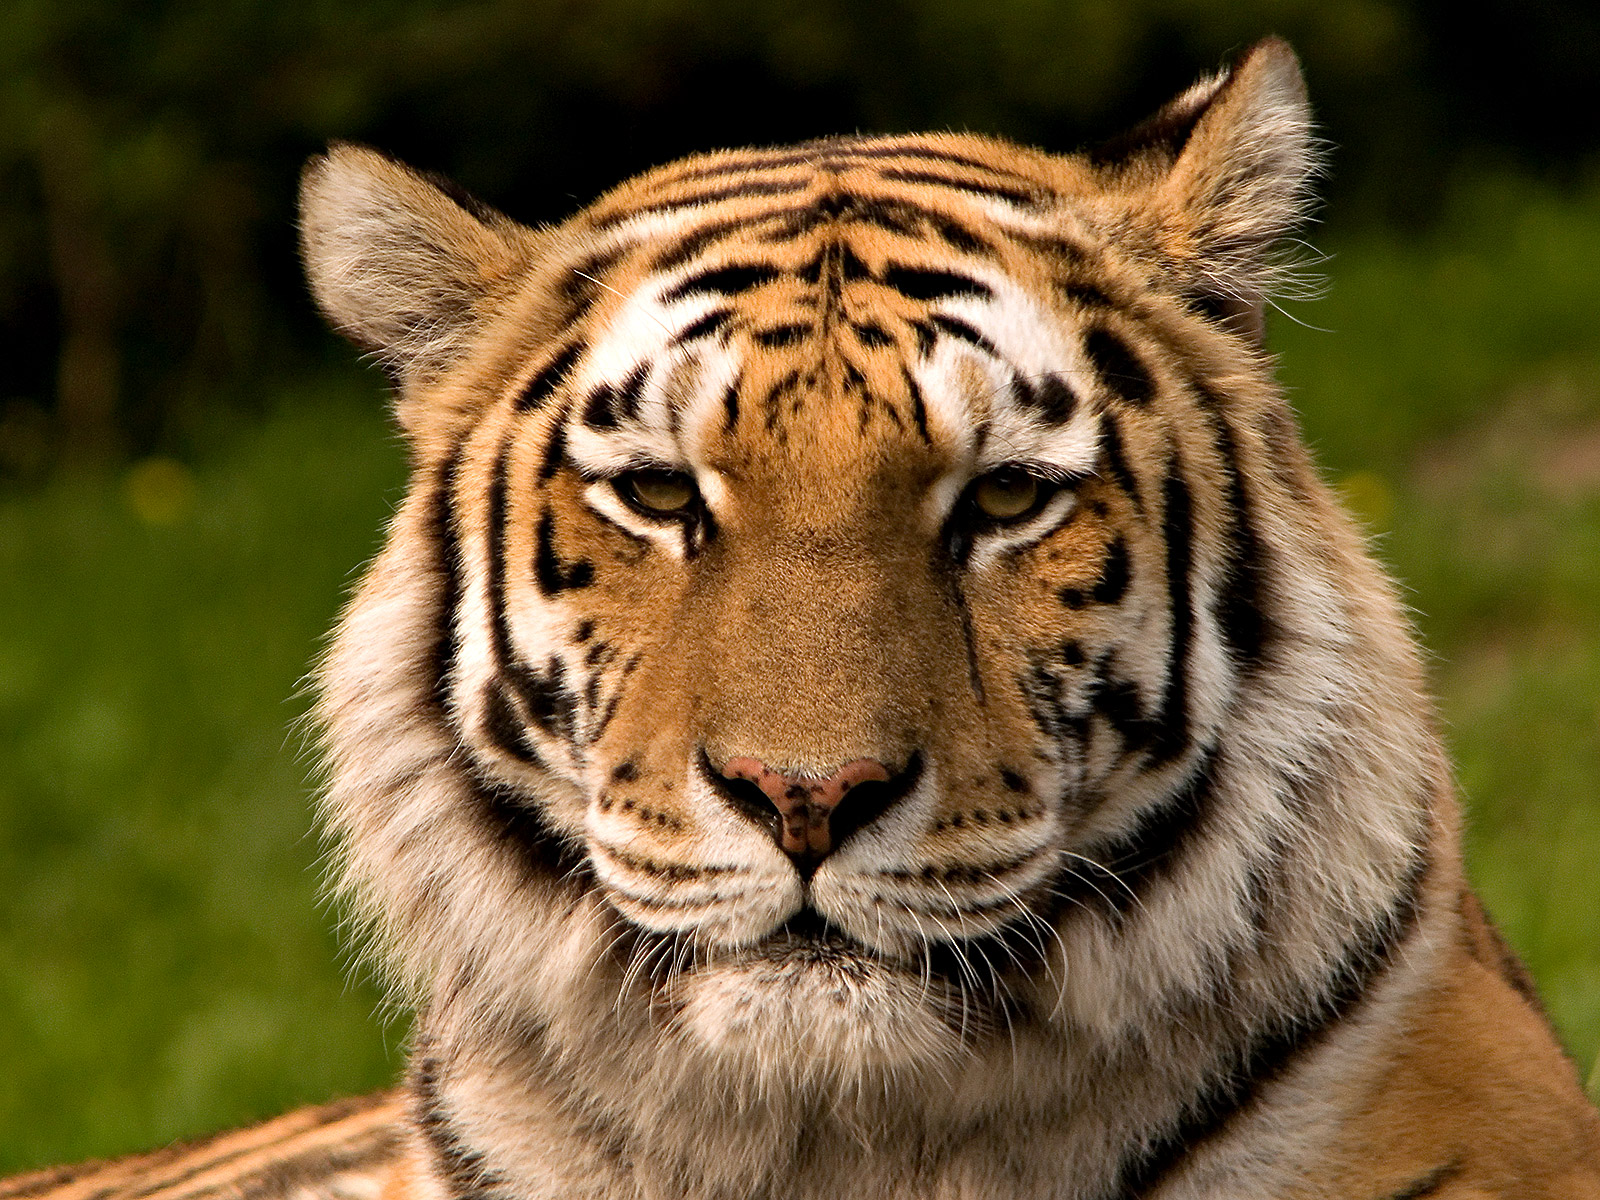
\includegraphics[width=0.5\textwidth]{fig/tiger.jpeg}
    \caption{\label{fig:tiger}A picture of a tiger.}
\end{figure}

Figure~\ref{fig:tiger} is a picture of a tiger.


%==========================================================================================
\subsection{Table}
\label{ss:Table}

\href{http://en.wikibooks.org/wiki/LaTeX/Tables}{Table examples on WIKIBOOKS}.

\begin{table}[htpb]\begin{center}
\caption{Table Example 1}
\begin{tabularx}{8cm}{llX}
\hline
Start & End  & Character Block Name \\
\hline
3400  & 4DB5 & CJK Unified Ideographs Extension A \\
4E00  & 9FFF & CJK Unified Ideographs \\
\hline
\end{tabularx}
 \end{center}\end{table}

\begin{table}[htpb]\begin{center}
\caption{Table Example 2}
\begin{tabular}{llr}
\hline
\multicolumn{2}{c}{Item} \\
\cline{1-2}
Animal & Description & Price (\$) \\
\hline
Gnat  & per gram & 13.65 \\
      & each     &  0.01 \\
Gnu   & stuffed  & 92.50 \\
Emu   & stuffed  & 33.33 \\
Armadillo & frozen & 8.99 \\
\hline
\end{tabular}
 \end{center}\end{table}
 
 \begin{table}[htpb]\begin{center}
	\label{t:prefix-table}
	\caption{Table Example 3}
	\renewcommand{\arraystretch}{1.0}
	\begin{tabularx}{300pt}{|c|X| }
		\hline
		\multirow{1}{*}{\textbf{Allocation}} &
		Allocation, Element, Type, Script 
		\\ \hline\hline
		%------------------------------
		\multirow{6}{*}{\textbf{Data Types}} &
        Byte2, Byte3, and Byte4\\ &
        Float2, Float3, Float4\\ &
        Int2, Int3, Int4\\ &
        Long2, Long3, Long4\\ &
        Matrix2f, Matrix3f, Matrix4f\\ &
        Short2, Short3, Short4
        \\ \hline\hline
		%------------------------------
		\multirow{4}{*}{\textbf{Graphics}} &
		Mesh\\&
		ProgramFragment, ProgramRaster\\&
		ProgramStore, ProgramVertex\\&
		RSSurfaceView
		\\ \hline
		%------------------------------
	\end{tabularx}
\end{center}\end{table}

\begin{table}[htpb]\begin{center}
\caption{Table Example 4}
\begin{tabular}{|l|l|l|}
\hline
\multicolumn{3}{|c|}{Team sheet} \\
\hline
Goalkeeper & GK & Paul Robinson \\ \hline
\multirow{4}{*}{Defenders} & LB & Lucus Radebe \\
 & DC & Michael Duberry \\
 & DC & Dominic Matteo \\
 & RB & Didier Domi \\ \hline
\multirow{3}{*}{Midfielders} & MC & David Batty \\
 & MC & Eirik Bakke \\
 & MC & Jody Morris \\ \hline
Forward & FW & Jamie McMaster \\ \hline
\multirow{2}{*}{Strikers} & ST & Alan Smith \\
 & ST & Mark Viduka \\
\hline
\end{tabular}
 \end{center}\end{table}
 
 \begin{table}[htpb]\begin{center}
\caption{Table Example 5}
 \begin{tabular}{l*{6}{c}r}
Team              & P & W & D & L & F  & A & Pts \\
\hline
Manchester United & 6 & 4 & 0 & 2 & 10 & 5 & 12  \\
Celtic            & 6 & 3 & 0 & 3 &  8 & 9 &  9  \\
Benfica           & 6 & 2 & 1 & 3 &  7 & 8 &  7  \\
FC Copenhagen     & 6 & 2 & 1 & 2 &  5 & 8 &  7  \\
\end{tabular}
 \end{center}\end{table}

%==========================================================================================
\subsection{Verb}
\label{ss:VerbUsage}
Let's take a overview on how to type special characters:\\
\verb|<FRAMEWORKS_BASE>/graphics/java/android/renderscript|\\\footnote{Path of <APP\_intermediates>: <ANDROID\_ROOT>/out/target/common/obj/APPS/APPNAME\_intermediates/}
You could also go back to the beginning of the chapter by the \hyperref[c:GetStarted]{\textbf{hyperref}}.

%==========================================================================================
\subsection{Enumeration}
\label{ss:Enumeration}
\begin{enumerate}
\item Enumerated Item1
\item Enumerated Item2
\item Enumerated Item3
\end{enumerate}

%==========================================================================================
\subsection{Code Display}
\label{ss:CodeDisplay}

\lstset{
	language=C++,
	stringstyle=\rmfamily,
	commentstyle=\itshape\color[rgb]{0.133,0.545,0.133},
	showstringspaces=false,
	basicstyle=\ttfamily\scriptsize,
	numberstyle=\tiny,
	numbers=left,
	stepnumber=1,
	numbersep=10pt,
	tabsize=2,
	breaklines=true,
	prebreak = \raisebox{0ex}[0ex][0ex]{\ensuremath{\hookleftarrow}},
	breakatwhitespace=false,
  	columns=fixed,
  	upquote=true,
  	extendedchars=true,
	xleftmargin=2em,
	xrightmargin=.5em,
	escapeinside={(*@}{@*)},
    mathescape=false,
}
Here is a "Hello, DanDing." example:
\begin{lstlisting}[style=nonumbers] 
void main(int argc, char **argv)
{
    printf("   ˊ_> ˋ  ");
}
\end{lstlisting}


Another example with line numbers:
\begin{lstlisting}
void main(int argc, char **argv)
{
    printf("   ˊ_> ˋ  ");
}
\end{lstlisting}

Matlab example:

\definecolor{dkgreen}{rgb}{0,0.6,0}
\definecolor{gray}{rgb}{0.5,0.5,0.5}
\lstset{language=Matlab,
   keywords={break,case,catch,continue,else,elseif,end,for,function,
      global,if,otherwise,persistent,return,switch,try,while},
   basicstyle=\ttfamily,
   keywordstyle=\color{blue},
   commentstyle=\color{red},
   stringstyle=\color{dkgreen},
   numbers=left,
   numberstyle=\tiny\color{gray},
   stepnumber=1,
   numbersep=10pt,
   backgroundcolor=\color{white},
   tabsize=4,
   showspaces=false,
   showstringspaces=false}

\begin{lstlisting}
function y = demo(x) % This is a comment.
   str = 'hello there';
   y = x + 1;
end
\end{lstlisting}

%==========================================================================================
\subsection{Math}
\label{ss:Math}
\begin{itemize}
    \item Inline mode:\\
The solution to $\sqrt{x} = 5$ is $x=25$.
    \item Display mode:\\
The solution to \[\sqrt{x} = 5\] is \[x=25.\]
    \item Numbered mode:
\begin{equation}
2+2=4
\end{equation}
    \item Non-numbered:
\begin{equation*}
2+2=4
\end{equation*}
    \item Aligning:
\begin{align*}
2x^2 + 3(x-1)(x-2) & = 2x^2 + 3(x^2-3x+2)\\
&= 2x^2 + 3x^2 - 9x + 6\\
&= 5x^2 - 9x + 6
\end{align*}
     \item Fractions:
\[
 \frac{n!}{k!(n-k)!} = \binom{n}{k}
\]
    \item Matrix:
\[
 A_{m,n} =
 \begin{pmatrix}
  a_{1,1} & a_{1,2} & \cdots & a_{1,n} \\
  a_{2,1} & a_{2,2} & \cdots & a_{2,n} \\
  \vdots  & \vdots  & \ddots & \vdots  \\
  a_{m,1} & a_{m,2} & \cdots & a_{m,n}
 \end{pmatrix}
\]
\end{itemize}
\href{http://en.wikibooks.org/wiki/LaTeX/Mathematics}{More examples on WIKIBOOKS}.


%==========================================================================================
\subsection{Algorithms}
\label{ss:Algorithms}
\begin{algorithm}[h]                      % enter the algorithm environment
\caption{Calculate $y = x^n$}          % give the algorithm a caption
\label{alg1}                           % and a label for \ref{} commands later in the document
\begin{algorithmic}                    % enter the algorithmic environment
    \Require $n \geq 0 \vee x \neq 0$
    \Ensure $y = x^n$
    \State $y \Leftarrow 1$
    \If{$n < 0$}
        \State $X \Leftarrow 1 / x$
        \State $N \Leftarrow -n$
    \Else
        \State $X \Leftarrow x$
        \State $N \Leftarrow n$
    \EndIf
    \While{$N \neq 0$}
        \If{$N$ is even}
            \State $X \Leftarrow X \times X$
            \State $N \Leftarrow N / 2$
        \Else[$N$ is odd]
            \State $y \Leftarrow y \times X$
            \State $N \Leftarrow N - 1$
        \EndIf
    \EndWhile
\end{algorithmic}
\end{algorithm}
\href{http://en.wikibooks.org/wiki/LaTeX/Algorithms_and_Pseudocode}{More examples on WIKIBOOKS}.


\chapter{Introduction}
\label{c:intro}

HiHi Iam r44~. The organization of this thesis is as follows. In chapte~\ref{c:thm}, the theoretical background and definition of surface plasmon will be included~\cite{maier2007plasmonics}. Chapte~\ref{c:exp} contains description of experiment methods such as atomic force microscopy and scanning electron microscopy. 


% Motivation

% Scenario

% Weakness of LeeWave.

% Contribution

\section{Thesis Overview}
\label{s:ThesisOverview}
In this section, we describe the overview of this thesis.

%\bibliographystyle{unsrt}
%\bibliography{thesisbib}
\chapter{Related Works}
\label{c:related}

%Overall

%CP

%PRP

%LeeWave
Now let's talk about the state-of-the-art method, LeeWave, which is the starting point of our framework. The spirit of LeeWave is to iteratively pruning impossible candidaites until only $k$ instances left by transforming a raw feature vector into an error tree like TODO with the help of the Haar wavelet transformation. Although the total number of coefficients in an error tree would be equal to length of the raw feature vector, the coefficients at the upper levels would be more important than those in the lower levels.  The importance defined here is the chance to contibute more to the final Euclidean distance,  And it could also be observed from the way to calculate the Euclidean distance from the error trees, the higher level the coefficient is, the heavier weight it has to multiply.

Once we have the importance of the coefficients, LeeWave sends coefficents according to their levels in the error tree transformed from the query $q$, from upside to down. In each round, LeeWave would send those coefficients in one level of the tree to each candidate machines.  Then, these machines would return some information that allows the server to compute the bounds between $q$ and the instances in these machines.  With the help of these bounds, the server could prune some instances that they are impossible to be the final answers.  If there are exactly $k$ instances left after pruning, then we just achive our goal to find the $k$NN/$k$FN.  Otherwise, the server would send the next level and repeat the pruning process until finding the answers or sending every level of this tree.
%MsWave

%\bibliographystyle{unsrt}
%\bibliography{thesisbib}
\chapter{Methodology}
\label{c:method}
In this chapter, we give the details about our framework.

%==========================================================================================
\section{Problem Setup}
\label{s:probsetup}
There are a query set $Q={\{q_1,q_2,...,q_T\}}\subset\mathbb{R}^D$ at the server $P$ and a dataset $X_i\subset\mathbb{R}^D$ on each local machine $M_i$, $\forall i=1,2,...,m$ where the total number of instances in these machines is $N$.  For each coming query $q_t$, we want to find its $k_{th}$ nearest neighborhood among these distributed datasets while reducing the transmission cost between $P$ and each $M_i$.

%==========================================================================================
\section{Overview of Our Framework}
\label{s:overview}
In this section, we describe an overview of our framework.  Then, we will give the details about the framework in the following sections.

\begin{figure}[htpb!]
  \centering
    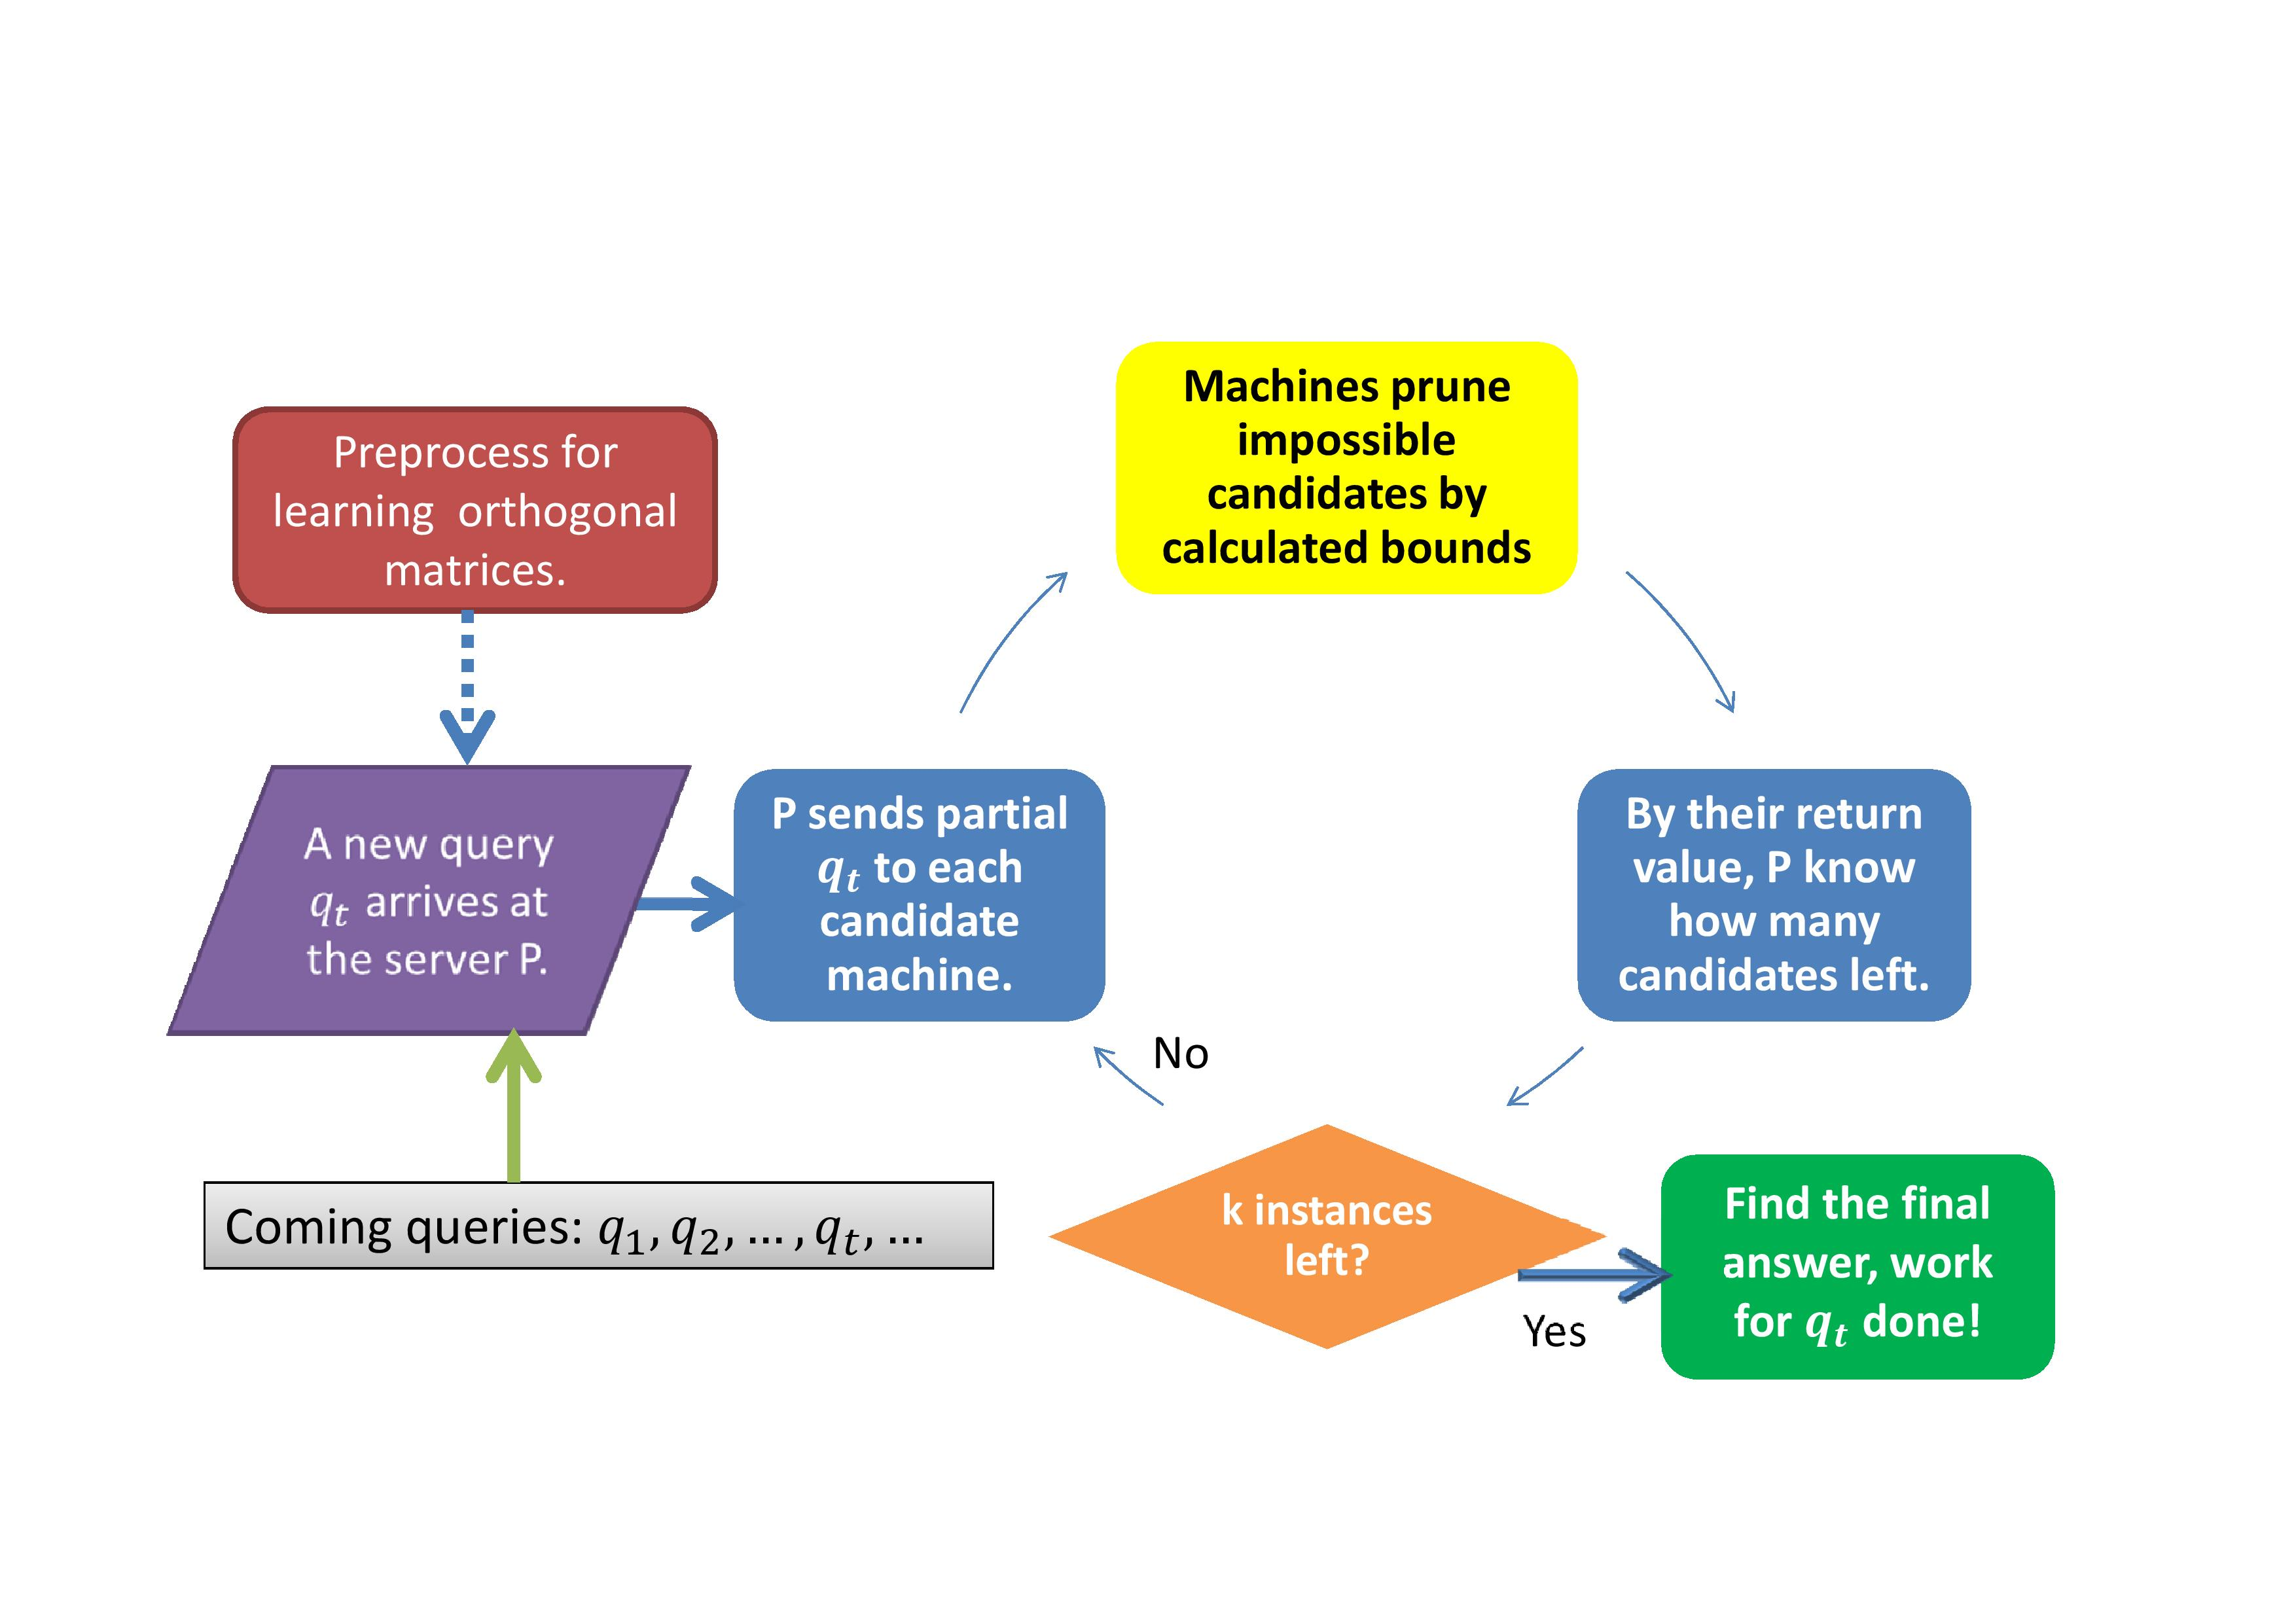
\includegraphics[width=0.75\textwidth]{fig/flow.jpg}
    \caption{\label{fig:overallflow}The overall flow of our framework.}
\end{figure}

Figure~\ref{fig:overallflow} is the overall flow on our framework.  There are two main phases in our framework.  For each $X_i$, the first phase (the red part) only needs to be done for once.  On the other hand, we need to run the second phase (the cycle) for each new query $q_t$.

The first phase is an preprocessing procedure for the second phase. Its goal is to improve the performance of pruning in the second phase.  We will prove in the section \ref{ss:derivation_of_the_bounds} that this pruning power is highly correlated to the distribution of the norm of the feature vectors. As a result, each $M_i$ would learn an othorogal matrix $W_i$ for its $X_i$ to fit our desired distribution and then send each $W_i$ back to $P$.  We can notice that this phase is only dependent on $X_i$ and independent of $q_t$.  Therefore, we only need to do the first phase for once.  we give the details about how to learn $W_i$, how to send it back to $P$ in the section \ref{ss:optimize_with_orthogonal_constraints}.

The second phase is the main procedure of our framework.  Note that $P$ have already got $W_i$ for each $X_i$ in the beginning of the second phase. For each coming query $q_t$, we iteratively prune some candidates which are impossible to be the $k$NN of $q_t$ to reduce the search space until there are only $k$ candidates left.

To prune candidates iteratively, we divide the second phase into several rounds.  For each round $j$, we use a function $S_i(q_t,j,\theta_t;W_i)$ to generate the values for trasmitting from $P$ to $M_i$, where $S_i$ is the importance-selecting function of $M_i$ and $\theta_t$ is its parameters for deciding how many elements we need to send.  (We put the details of $S_i$ at the section \ref{ss:importance_selecting_function}.)  By these values, each $M_i$ could calculate the bounds between each candidate $x_l$ and $q_t$.  With these bounds, $P$ would be able to determine which candidates are definitely not our answers and then disregards them in the following rounds.  By these pruning, we could achieve the goal of saving transmission cost from avoiding to consider the unnecessary candidates.

Note that we could use the square of the Euclidean distance instead of the origin Euclidean distance to find $k$NN as it is non-negative.  So we will use the former one in our framework.

%==========================================================================================
\section{First Phase}
\label{s:first_phase}

In this section, we talk about the first phase of our framework.
%==========================================================================================
\subsection{Definition of Ortohogonal Transformation}
\label{ss:ortho_def}

The most important part of the first phase is the orthogonal transformation.  So we give its definition as below.

\newtheorem{Orthogonal}{\bf Definition}
\begin{Orthogonal}
\normalfont
A matrix $W \in\mathbb{R}^{D\times D}$ is orthogonal if whose columns and rows are orthogonal vectors, i.e.
\[
W^{T}W=WW^{T}=I
\]
where $I$ is the identity matrix.
\end{Orthogonal}

%==========================================================================================
\subsection{Property of Orthogonal Transformation}
\label{ss:ortho_prop}

There are some useful properties in orthogonal transformation.  Here we introduce the one that we will use in the derivation of our bounds.

\newtheorem{ProOfOrthogonal}{\bf Property}
\begin{ProOfOrthogonal}
\normalfont
Let $x, y\in\mathbb{R}^{D\times 1}$, and $W\in\mathbb{R}^{D\times D}$ be an orthogonal matrix. Then,
\[
Dist(x,y)=\sum^D_{d=1}{(x[d]-y[d])^2} \\
=\sum^D_{d=1}{(W[d,:]x-W[d,:]y)^2}=Dist(Wx,Wy)
\]
where $W[d,:]$ is the $d_{th}$ row of $W$.
\end{ProOfOrthogonal}

We will use this important property in the section~\ref{sub:equivalent_bounds_after_transformation}.

%==========================================================================================
\section{Enhance the Bounds by the Orthogonal Transformation}
\label{s:ortho_bounds}
In the section \ref{s:overview}, we mentioned that the first phase is an auxiliary step for the second phase.  After the introduction of the orthogonal transformation, we introduce this powerful tool into the first phase in our framework.

\subsection{The Goal of the First Phase} % (fold)
\label{ss:the_goal_of_the_first_phase}

Our goal in the first phase is to reduce the ranges of the bounds used in the second phase.  Since we will use a threshold to prune the impossible candidates according to their bounds in the pruning procedure, the ranges of the bounds would be one of the most influential factor of the pruning power. It is easy to understand that when the ranges of their bounds is short, more candidates would be pruned than those with long ranges of the bounds.  In other words, the shorter the range of the bound, the higher chance this candidate would be pruned if it is not our final answer of $k$NN.  

Moreover, we would prove in the section~\ref{ss:reduce_the_norm_with_orthogonal_transformation} that to reduce the range of the bounds, the final goal of the first phase would become to learn an orthogonal transformation $W$ which could make each raw feature vector $x\in \mathbb{R}^D$ (the orange vector in the figure \ref{fig:vector}) transformed to be $Wx$ (the red vector in the figure \ref{fig:vector}) which would make the absolute values of elements in the forward part of the vector much larger and those in the later part much smaller.
\begin{figure}[htpb!]
  \centering
    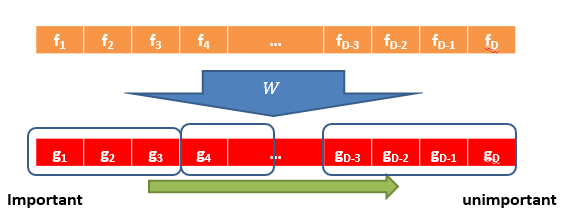
\includegraphics[width=0.8\textwidth]{fig/important.png}
    \caption{\label{fig:vector}The goal of the first phase.}
\end{figure}


% subsection the_goal_of_the_first_phase (end)

\subsection{Definition of the Bounds} % (fold)
\label{ss:definition_of_the_bounds}

Before we explain why we need the orthogonal transformation to enhance our bounds, we need to define our bounds for the pruning.  Recall that given a query $q_t$, our goal is to find its $k$NN in these distributed datasets $X_i$.  Intuitively, we need to calculate the square of the Euclidean distance $Dist(q_t,x), \forall x\in \cup_i X_i$.  However, to cacluate $Dist(q_t,x)$, we need to send the whole $q_t$ to the local machines or send the whole $x$ to $P$, which causes a huge transmission cost.  Therefore, instead of the exact value of Euclidean distances, our propsed framework uses bounds to confine this distance for finding the $k$NN.

\newtheorem{Bounds}{\bf Definition}
\begin{Bounds}
\normalfont
$\forall x,y \in \mathbb{R}^D$, a lower bound $LB(x,y)$ and a upper bound $UB(x,y)$ must satisfy the following inequation:
\[
LB(x,y)\leq Dist(x,y) =\sum^D_{d=1}{(x[d]-y[d])^2} \leq UB(x,y)
\]
\end{Bounds}

\subsection{Relation Between the Norms and the Bounds} % (fold)
\label{sub:relation_between_the_norms_and_the_bounds}

To acheive the goal of reducing the length of the ranges of the bounds, we could look into the derivation of the bounds. Suppose there are two vectors $x,y\in \mathbb{R}^D$, but we could only observe the first $s$ dimensions of $x$ and $\sum^D_{d=s+1}{x[d]^2}$, which is the square of two norm of the unobserved part $x[s+1:D]$.  In the section \ref{ss:derivation_of_the_bounds}, we derive the bounds as 
{
\begin{eqnarray*}
\lefteqn{LB(x,y) = \sum^s_{d=1}{(x[d]-y[d])^2}.} \label{eq:single-LB-tmp} \\
\lefteqn{UB(x,y) = \sum^s_{d=1}{(x[d]-y[d])^2}} \notag \\
& + & \sum^D_{d=s+1}{x[d]^2}+\sum^D_{d=s+1}{y[d]^2} \notag \\
& + & 2 \times \sqrt{\sum^D_{d=s+1}{x[d]^2}\times \sum^D_{d=s+1}{y[d]^2}.}\label{eq:single-UB-tmp}
\end{eqnarray*}
}

Therefore, we could get the length of the range by the substraction.
{
\begin{eqnarray*}
\lefteqn{Len = UB(x,y) - LB(x,y)}\\
& = \sum^D_{d=s+1}{x[d]^2}+\sum^D_{d=s+1}{y[d]^2} \\
& + 2 \times \sqrt{\sum^D_{d=s+1}{x[d]^2}\times \sum^D_{d=s+1}{y[d]^2}.}\label{eq:len-range}
\end{eqnarray*}
}
Since the term $\sum^D_{d=s+1}{x[d]^2}$ is given, all we could do to reduce the length is to make use of the $\sum^D_{d=s+1}{y[d]^2}$ term.  If we could reduce $\sum^D_{d=s+1}{y[d]^2}$, the term $\sum^D_{d=s+1}{x[d]^2}\times \sum^D_{d=s+1}{y[d]^2}$ would also decrease and then make $Len$ smaller.  Therefore, our goal now becomes to make the term $\sum^D_{d=s+1}{y[d]^2}$ as small as possible, which is the square norm of the vector $y[s+1:D]$.

Note that the lower (upper) bounds is non-decreasing (non-increasing) as $s$ becomes larger and $LB(x,y)=UB(x,y)$ when $s=D$.  This means that $LB$ and $UB$ would be exactly equal to $\sum^D_{d=1}{(x[d]-y[d])^2}$ eventually.

To reduce the length of the ranges $Len$ for each $s$, we hope to make $\sum^D_{d=s+1}{y[d]^2}$ as small as possible.  However, since the feature vector $y$ is given from datasets, the value of $\sum^D_{d=s+1}{y[d]^2}$ is already  determined when $s$ is given.  As a result, we introduce the orthogonal transformation to achieve this goal.

% subsection relation_between_the_norms_and_the_bounds (end)


\subsection{Equivalent Bounds After Transformation} % (fold)
\label{sub:equivalent_bounds_after_transformation}

From the section \ref{ss:ortho_prop}, we know the distance of two vectors won't be changed after an orthogonal transformation.  Now we use this property to achieve our goal to reduce the length of the ranges $Len$ given $s$.

Given an orthogonal transformation $W\in\mathbb{R}^{D\times D}$, we have $Dist(x,y)=Dist(Wx,Wy)$.  This means that the bounds we derivated before could also be the bounds for $Dist(Wx,Wy)$.  That is,
\[
LB(x,y)\leq Dist(x,y)=Dist(\hat{x},\hat{y}) \leq UB(x,y)
\]
where $\hat{x}=Wx$.

This also means that we could use the same way to derivate the lower bounds and upper bounds for $Dist(Wx,Wy)$ and these bounds are also the bounds for $Dist(x,y)$.  That is,
\[
LB(\hat{x},\hat{y})\leq Dist(x,y)=Dist(\hat{x},\hat{y}) \leq UB(\hat{x},\hat{y})
\]

So, we could use the bounds $LB(\hat{x},\hat{y}),UB(\hat{x},\hat{y})$ to confine $Dist(x,y)$ and the length of range we want to reduce becomes
{
\begin{eqnarray*}
\lefteqn{\hat{Len}(W) = UB(\hat{x},\hat{y}) - LB(\hat{x},\hat{y})} \\
& = \sum^D_{d=s+1}{\hat{x}[d]^2}+\sum^D_{d=s+1}{\hat{y}[d]^2} \notag \\
& +  2 \times \sqrt{\sum^D_{d=s+1}{\hat{x}[d]^2}\times \sum^D_{d=s+1}{\hat{y}[d]^2}.}\label{eq:len-range-hat}
\end{eqnarray*}
}
which becomes a function of $W$.

As a result, instead of trying to reduce $\sum^D_{d=s+1}{y[d]^2}$ which is impossible as we mentioned in the section \ref{sub:relation_between_the_norms_and_the_bounds}, our goal becomes to reduce $\sum^D_{d=s+1}{\hat{y}[d]^2}$ with the help of $W$.

% subsection equivalent_bounds_after_transformation (end)

\subsection{Reduction of the Norm with Orthogonal Transformation} % (fold)
\label{ss:reduce_the_norm_with_orthogonal_transformation}

For $y\in \mathbb{R}^{D\times 1}$ and $W\in\mathbb{R}^{D\times D}$, given $s$, we want to reduce $\sum^D_{d=s+1}{\hat{y}[d]^2}$ as much as possible.  However, since $s$ is unknown while deciding $W$ in the first phase of our framework, we have to handle all possible values which $s$ could be.  Moreover, since $\sum^D_{d=1}{\hat{y}[d]^2}$ is equal to $\sum^D_{d=1}{y[d]^2}$, which is independent with $W$, if the $\sum^D_{d=s+1}{\hat{y}[d]^2}$ decreases with some $W$, the term $\sum^s_{d=1}{\hat{y}[d]^2}$ must increase.  Here, we use a more general strategy to deal with these problems.

We could look the term $\sum^D_{d=s+1}{\hat{y}[d]^2}$ from a different angle.  Actually, this term is the square norm of the latter part of the vector $\hat{y}$. Therefore, although $\sum^D_{d=1}{\hat{y}[d]^2}$ is a constant for $W$, we could reduce the square norm of the latter part by increasing the forward part of it.  In other words, we move the norm of the latter part of $y$ to its forward part.  To accomplish it, we design an objective function and then optimize this function to find our ideal $W$.

\begin{equation}\label{objective}
	f(W;y)=\sum^D_{d=1}{w_d\times\hat{y}[d]^2}=\sum^D_{d=1}{w_d\times(W[d,:]y[d])^2}
\end{equation}
where $w_d=d,  \forall d=1,2,\ldots,D.$.

Because $w_d$ would give the larger penalty as $d$ increases, the elements in the latter part of $\hat{y}$ would be forced to become small while minimizing this objective function.  This is exactly our goal to reduce $\sum^D_{d=s+1}{\hat{y}[d]^2}$.  Therefore, our question becomes how to optimize this objective function with the constraints that $W$ must be an orthogonal matrix.


% subsection reduce_the_norm_with_orthogonal_transformation (end)

\subsection{Optimization over Orthogonal Constraints} % (fold)
\label{ss:optimize_with_orthogonal_constraints}

Finally, we could introduce this concept of reducing the norms into our framework.  In the first phase, we solve the following optimization problem to learn an orthogonal matrix $W_i$ for each machine $Mi$.

\begin{equation}\label{objective-F}
\begin{aligned}
& \underset{W}{\text{minimize}}
& & F_i(W) \\
& \text{subject to}
& & W^{T}W=WW^{T}=I
%& & W \leq b_i, \; i = 1, \ldots, m.
\end{aligned}
\end{equation}

where 
\begin{equation}
	F_i(W)=\sum_{x \in X_i}{f(W;x)}\\
	=\sum_{x \in X_i}{ \sum^D_{d=1} {d\times(W[d,:]x[d])^2} }
\end{equation}.

This is an optimization problem with constraints that its solution must be an orthogonal matrix.  We could solve it efficiently with the help of the package from~\cite{Fopt} as long as we have its gradient. 

After we get the optimal $W^*_i$ for each $M_i$, we send these matrices back to the server $P$.  Since the learning of $W^*_i$ is independent with the queries in the future, we only have to go through the procedure of learning $W^*_i$ for once if $X_i$ doesn't change too much.  Then our first phase is done.

% subsection optimize_with_orthogonal_constraints (end)

\subsection{Reduce the Cost of Sending Matrices} % (fold)
\label{ss:reduce_the_cost_of_sending_matrices}
%http://math.stackexchange.com/questions/375344/parameters-to-represent-degrees-of-freedom-in-n-times-n-orthogonal-real-matric
%http://math.stackexchange.com/questions/28189/freedoms-of-real-orthogonal-matrices

However, the cost to sending an orthogonal matrix $W\in\mathbb{R}^{D\times D}$ is $D\times D$, which is too expensive.  Therefore, in this section, we prove that we could reduce this cost to $\frac{D\times (D-1)}{2}$.

First, we introduce a lemma which would be used in our proof.

\newtheorem*{lemma}{Lemma}
\begin{lemma}\normalfont
 For a vector $\bold{x}=(x_1,x_2,\ldots,x_D)\in\mathbb{R}^D$, we could use a spherical coordinate system with a radial coordinate $r$ and $D-1$ angular coordinates $\phi_1, \phi_2, ..., \phi_{D-1}$ to represent it as
\begin{itemize}
	\item $x_1 = r \cos(\phi_1)$
	\item $x_2 = r \sin(\phi_1)\cos(\phi_2)$
	\item $x_3 = r \sin(\phi_1)\sin(\phi_2)\cos(\phi_3)$
	\item ~\vdots
	\item $x_{D-1} = r \sin(\phi_1)\ldots \sin(\phi_{D-2})\cos(\phi_{D-1})$
	\item $x_{D} = r \sin(\phi_1)\ldots \sin(\phi_{D-2})\sin(\phi_{D-1})$
\end{itemize}
where $\phi_i\in[0,\pi],~\forall i=1,2,...,D-2$ and $\phi_{D-1}\in[0,2\pi)$. $\blacksquare$
\end{lemma}

Since these row vectors $w_1,w_2,w_3,\ldots,w_D$ in $W$ are orthonomal vectors, their $r$ in this lemma is $1$, which allows us to represent an orthonomal vector in $\mathbb{R}^D$ with $D-1$ parameters ($\phi_1,\phi_2, ...,\phi_{D-1}$ in the lemma).  Moreover, since they are orthogonal to each other ($w_iw_j^T=0,~\forall i\neq j$), our goal becomes how to represent $D$ vectors in $\mathbb{R}^D$ which are orthogonal to each other.

Now we are ready to give the proof by mathematical induction.

\newtheorem*{half}{Theorem}
\begin{half}\normalfont
%Given an orthogonal transformation $W\in\mathbb{R}^{D\times D}$, we could use $\frac{D\times (D-1)}{2}$ parameters to construct $W$.
Given $D$ orthonomal vectors $w_1,w_2,w_3,\ldots,w_D \in \mathbb{R}^D $, we could use $\frac{D\times (D-1)}{2}$ parameters to represent them.
\end{half}

\newtheorem*{mproof}{Proof}
\begin{mproof}\normalfont

\emph{Base case}: \\
If $d=2$, we could use a single parameter $\theta$ for $w_1, w_2$ as

\begin{equation}
\begin{aligned}
& w_1 = ( \cos\theta,\sin\theta ) \\
& w_2 = ( \cos(\theta + \frac{\pi}{2}),\sin(\theta + \frac{\pi}{2}) )
\end{aligned}
\end{equation}

Therefore, the total number of parameters here is $1$ and equal to $\frac{2\times (2-1)}{2}$.
\\ \\
To be clear, we give one more base case here.
\\ 
\emph{Base case-2}:\\
When $d=3$, we need to represent three vectors $w_1,w_2,w_3\in \mathbb{R}^3$.

In the beginning, by the lemma above, we could use $3-1=2$ parameters to represent $w_3$.  \\
Then, since $w_1$ and $w_2$ are orthogonal to $w_3$, they must lie in the plane whose normal vector is $w_3$.  Since we already have $w_3$ (with two parameters), this plance is fixed.  All we need to do is to decide $w_1$ and $w_2$ on this $\mathbb{R}^2$ plane.  By projecting the $x$ axis in the $\mathbb{R}^3$ to this plane, we could build a Cartesian coordinate system in two dimensions on this plane. And we know that we could use one parameter to decide $w_1$ and $w_2$ in an $\mathbb{R}^2$ plane from the base case above.

So, the total number of parameters for $\mathbb{R}^3$ case is $2+1=3$ and equal to $\frac{3\times (3-1)}{2}$
\\ \\
\emph{Inductive hypothesis}: \\
Suppose the theorem holds for all values $d$ up to some $k$, $k > 3$
\\ \\
\emph{Inductive step}: \\
Let $d=k+1$, we need to represent $k+1$ vectors $w_1,w_2,w_3,\ldots,w_{k+1}\in \mathbb{R}^{k+1}$. We could use similar way like $d=3$ to do it.

First, by the lemma above, we could use $(k+1)-1=k$ parameters to represent $w_{k+1}$.  \\
Then, our problem becomes to decide $w_1,w_2,\ldots,w_k$ on this hyperplane whose normal vector is $w_{k+1}$.  From the inductive hypothesis, we know it needs $\frac{k\times (k-1)}{2}$ parameters.

So, the total number of parameters for $\mathbb{R}^{k+1}$ case is 
\[
k + \frac{k\times (k-1)}{2} = \frac{k\times (k+1)}{2}
\ldots\blacksquare
\]
\end{mproof}
% subsection reduce_the_cost_of_sending_matrices (end)


%==========================================================================================
\section{Second Phase}
\label{s:prune}
Now we start to discuss the second phase of our framework.  In this section, we talk about how to prune the candidates if we already have bounds.  Note that this mechanism is the most crucial part to achieve our goal to save the transmission cost.

% subsection definition_of_bounds (end)

\subsection{Pruning the Candidates with the Bounds} % (fold)
\label{ss:prune_the_candidates_with_the_bounds}

For the query $q_t$, if we already know $LB(q_t,x)$ and $UB(q_t,x)$ $\forall x\in \cup_i X_i$, we could use the $k_{th}$ smallest upper bounds and directly prune those instances whose lower bounds are higher than this value $thr$. I.e., we want to prune
\[
\{x~|LB(q_t,x)>thr, \forall x \in \cup_i X_i\}
\]
where $thr$ is the $k_{th}$ largest $UB(q_t,x)$ $\forall x\in \cup_i X_i$.  The following figure~\ref{fig:prune} is an example of how we prune impossible instances.

\begin{figure}[htpb!]
  \centering
    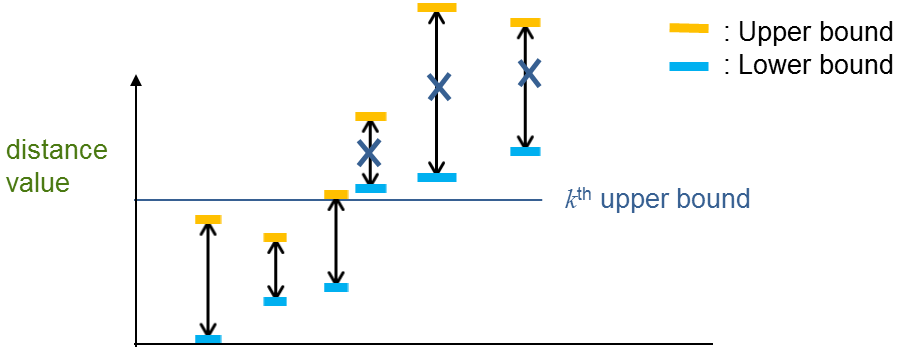
\includegraphics[width=1.0\textwidth]{fig/prune.png}
    \caption{\label{fig:prune}The procedure of pruning impossible candidates.}
\end{figure}

We will talk about the details of calculation these bounds and finding the threshold $thr$ in the section \ref{ss:find_the_threshold_in_distributed_machines}.

% subsection prune_the_candidates (end)

\subsection{Derivation of our Bounds} % (fold)
\label{ss:derivation_of_the_bounds}

Suppose there are two vectors $x,y\in \mathbb{R}^D$, we know the square of their Euclidean distance is 
\begin{equation}
	Dist(x,y)=\sum^D_{d=1}{(x[d]-y[d])^2}
\end{equation}

However, if we could only observe the first $s$ dimensions of $x$, we could decompose their distance as 

\begin{equation}\label{eq:Eu_decomp}
\begin{aligned}
& Dist(x,y)=\sum^D_{d=1}{(x[d]-y[d])^2}  \\
& =\sum^s_{d=1}{(x[d]-y[d])^2} + \sum^D_{d=s+1}{(x[d]-y[d])^2}
\end{aligned}
\end{equation}

Since the first component of \eqref{eq:Eu_decomp} is already known, all we need to do is to deal with the second term. Therefore, we further expand the second term as below:
\[
\sum^D_{d=s+1}{(x[d]-y[d])^2}=\sum^D_{d=s+1}{x[d]^2}+\sum^D_{d=s+1}{y[d]^2}-\sum^D_{d=s+1}{2\times x[d]\times y[d].}
\]

By this analysis, we find the final term $\sum^D_{d=s+1}{x[d]\times y[d]}$ is the inner product between two partial vector $x[s+1:D]$ and $y[s+1:D]$, which could be approximated by Cauchy–Schwarz inequality
\begin{equation}\label{eq:Cauchy}
	\sum^D_{d=s+1}{x[d]\times y[d]} \leq \sqrt{\sum^D_{d=s+1}{x[d]^2}\times \sum^D_{d=s+1}{y[d]^2}.}
\end{equation}

After combing with \eqref{eq:Eu_decomp} and \eqref{eq:Cauchy}, we derive the bounds as 
{
\begin{eqnarray}
\lefteqn{LB(x,y) = \sum^s_{d=1}{(x[d]-y[d])^2}.} \label{eq:single-LB} \\
\lefteqn{UB(x,y) = \sum^s_{d=1}{(x[d]-y[d])^2}} \notag \\
& + & \sum^D_{d=s+1}{x[d]^2}+\sum^D_{d=s+1}{y[d]^2} \notag \\
& + & 2 \times \sqrt{\sum^D_{d=s+1}{x[d]^2}\times \sum^D_{d=s+1}{y[d]^2}.}\label{eq:single-UB}
\end{eqnarray}
}
We could notice that the calculation of the bounds only needs the first $s$ dimensions of $x$ and $\sum^D_{d=s+1}{x[d]^2}$.  Therefore, we only need one more number $\sum^D_{d=s+1}{x[d]^2}$ to get the bounds for the unobserved part $x[s+1:D]$.

% subsection derivation_of_bounds (end)

\subsection{Calculation of our Bounds} % (fold)
\label{sub:calculation_the_bounds}
After the derivation of the bounds, we describe the procedure of cacluating them in our framework.  

For the query $q_t$, at the first round (i.e. $j=1$), $P$ sends the first $s_1$ dimensions of $q_t$ and $\sum^D_{d=s_1+1}{q_t[d]}^2$ to each $M_i$ .  With these values, each $M_i$ would be able to calculate the lower bounds $LB_1(q_t,x)$ and upper bounds $UB_1(q_t,x)$ for each $x\in X_i$.  Then, after $P$ getting the $k_{th}$ smallest upper bounds as $thr$, we could run the pruning procedure.

In each following round (i.e. $j>1$), $P$ sends the next $s_j$ dimensions of $q_t$ to each $M_i$ whose instances were not pruned completely.  These $M_i$ will update their bounds as follows:

\begin{equation}
\begin{aligned}
& LB_j(q_t,x) = LB_{j-1}(q_t,x)+\sum^{p_j}_{d=p_{j-1}+1}{(q_t[d]-x[d])^2}. \\
& UB_j(q_t,x) = LB_{j}(q_t,x) \notag \\
& +  \sum^D_{d=p_j+1}{q_t[d]^2}+\sum^D_{d=p_j+1}{x[d]^2} \notag \\
& + 2 \times \sqrt{\sum^D_{d=p_j+1}{q_t[d]^2}\times \sum^D_{d=p_j+1}{x[d]^2}.}
\end{aligned}
\end{equation}

where $p_j=\sum^j_{i=1}{s_i}$, $LB_j$ and $UB_j$ indicate the lower bounds and upper bounds at the round $j$ repectively.

We call those $p_j$ as pivots, which mean that each machine would observe the first $p_i$ elements of $q_t$ at the round $j$.  

% subsection calculation_the_bounds (end)
\providecommand{\myceil}[1]{\left \lceil #1 \right \rceil }
\providecommand{\myfloor}[1]{\left \lfloor #1 \right \rfloor }

\subsection{Finding the Threshold in Distributed Machines} % (fold)
\label{ss:find_the_threshold_in_distributed_machines}
The question now is to find the threshold $thr$ for pruning. We know that $thr$ is the $k_th$ upper bounds in all bounds of these round. However, these bounds are calculated by each local machine and lied there.  That means we have to find it from a distributed data. In ~\cite{MsWave}, we directly send these bounds computed in each $M_i$ back to the server $P$.  However, it would make the transmission cost grow linearly with the number of total instances in these distributed machines and lead to expensive cost when our dataset is extremely huge.  As a result, we propose a method that could make the growth of the cost independent with the number of total instances.

To be simplified, we could think this problem as follows: given many distribued numbers $N_i$, we want to find the $k_{th}$ largest number among these $N_i$.  The $N_i$ here actually means the upper bounds at the machine $M_i$ in our framework.  Once we model this problem as this, we could solve it through modifying the work of \cite{PRP}.

In \cite{PRP}, there are also many phases to find the $k$NN.  In the first phase, the server $P$ would send the whole query to every machine.  Then, in the following phases, it just focuses on finding the instances with the $k_{th}$ largest distance with the query.  To make it fit our problem, we can only use the phases of PRP except the first phase to find the $k_{th}$ largest upper bound as our threshold $thr$.  Its cost is linear to
\[
m\times (\myfloor{\frac{k}{m}}+1),
\] which is much lower than \cite{MsWave} when the number of total instances is very large.

%we could estimate the total transmission cost for the single query as following
%\[
%	Cost = \sum^L_{i=1}{T_i\times ResSite_i}+\sum^L_{i=1}{2s_i}
%\]  
%where $T_i$ is the length $q_t$ which was sent , $ResSite_i$ is the number of residual machines, and $s_i$ is the number of residual candidates at the round $i$.


% subsection find_the_threshold_in_distributed_machines (end)
%==========================================================================================

\section{Decision of the Pivots} % (fold)
\label{s:decide_the_pivots}

The remaining problem is to decide how many dimensions (i.e. $s_j$) of $\hat{q_t}$ we have to send from the server $P$ in each round $j$.  If we send too few dimensions, the bounds would be too loose to prune any candidates and we will spend much unnecessary cost in finding the thresholds.  On the other hand, if we send too many dimensions, although it could allow us to prune many candidates at once, it would send too many dimensions to some candidates which could be pruned by much fewer dimensions.  That would also lead to the waste the transmission cost.  Therefore, in this section, we propose a simple but effective method to decide how many dimensions of $\hat{q_t}$ we should send from $P$ in each round.


\subsection{Estimation of the Number of Residual Machines} % (fold)
\label{ss:estimate_the_number_of_residual_machines}

From the discussion above, we could notice that the decision of pivots is highly dependent on the transmission cost.  Therefore, if we could estimate the cost as a cost function of the pivots $p_j$, we could decide these pivots by optimizing this function.

However, to estimate the cost, we need to know the number of residual candidates machines before sending those dimensions of $\hat{q_t}$ in each round.  But it is almost impossible to know how many machines would be left after we send part of $\hat{q_t}$ before we actually send the part of $\hat{q_t}$.  Therefore, we estimate a vector called $EstResMach \in\mathbb{R}^D$ where $EstResMach[j]$ indicates our estimate of the number of residual machines \emph{after} we send $\hat{q_t}[1:j]$ to each local machine.  

To allow $P$ to  estimate this vector $EstResMach\in\mathbb{R}^D$ without causing any more transmission cost, we use the history information from $\hat{q_1},\ldots,\hat{q_t}$.  Suppose that we just finish finding the answer for $\hat{q_t}$, during the procedure, we would collect some such pairs of information $(index_j, ResMach_j)$ for some $j$ where $index_j$ means each candidate machine would observe the first $index_j$ dimensions of $\hat{q_t}$ at the round $j$ and $ResMach_j$ indicates the number of residual machines after pruning by $\hat{q_t}[1:index_j]$.  For those dimensions which are not in these pairs, we use linear interpolation to estimate their $ResMach$.  

Figure \ref{fig:LI} is an example for the above procedure.  The blue vector means the pairs of information we collected for $\hat{q_t}$ as $(2,400),~(4,390),\ldots,~(D-3,15),~(D-1,13),~(D,1)$.  And the red vector is the results after linear interpolation.

\begin{figure}[htpb!]
  \centering
    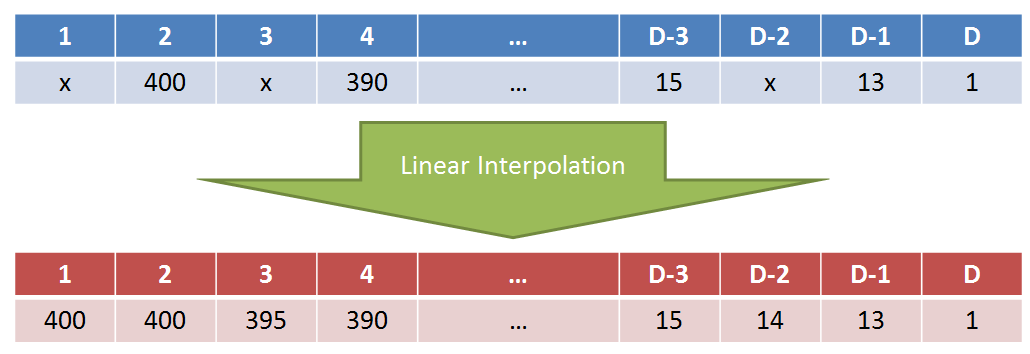
\includegraphics[width=1.0\textwidth]{fig/LI.png}
    \caption{\label{fig:LI}The example of linear interpolation.}
\end{figure}

By average this vector (the red one) collected from every query as $EstResMach$, $P$ could estimate the number of residual machines \emph{before} sending a query.


% subsection estimate_the_number_of_residual_machines (end)

\subsection{Estimation of the Transmission Cost} % (fold)
\label{ss:estimate_the_transmission_cost}

Once we have the vector $EstResMach$, we are ready to estimate the transmission cost \emph{before} sending the query.  For a query, we could estimate its transmission cost in the first round 
\[
Cost_1 = m\times s_1 + Cost_{PRP}(m)
\]
And for those round $j>1$ as follows,
\[
Cost_j = EstResMach[p_{j-1}]\times s_j + Cost_{PRP}(EstResMach[p_{j-1}])
\]
where $p_j=\sum^j_{i=1}{s_i}$.

The term $m\times s_1$ means the cost to send part of $\hat{q_t}$ in the first round which is the length of this part times the total number of machines.  Similarily, the term $EstResMach[p_{j-1}]\times s_j$ is the cost to send the next part of $\hat{q_t}$ in the round $j$ to the residual machines.  On the other hand, the term $Cost_{PRP}(i)$ is the total cost to find the threshold $thr$ and then send it to all $i$ residual machines. Therefore, we could minimize the total cost to get the optimal pivots.

However, since there are $D$ dimensions could be picked .there are too many variables to decide in this problem.  According to our experiments, the most crucial variable is the number of dimensions which will be sent in the first round, which is $s_1$ in this optimization problem.  The other $s_j$ don't have such huge influence like $s_1$.  Therefore, we make all $s_j$ be equal and then simplifiy this optimization problem as follows,

\begin{equation}
\begin{aligned}
& \underset{StartD, EachLenD}{\text{minimize}}
~\sum_j{Cost_j(StartD,EachLenD)} \\
& \text{subject to}
~StartD, EachLenD \in \mathbb{N}\\
\text{where} \\ 
\end{aligned}
\end{equation}

\[
Cost_1 = m\times StartD + Cost_{PRP}(m) \\
\]
\[
Cost_j = EstResMach[p_{j-1}]\times EachLenD + Cost_{PRP}(EstResMach[p_{j-1}]), \forall j>1\\
\]
\[
p_j=StartD + (j-1)\times EachLenD.
\]

% subsection estimate_the_transmission_cost (end)

\subsection{Coordinate Descent to Decide the Pivots} % (fold)
\label{ss:coordinate_descent_to_decide_the_pivots}

Now we have reduced the number of variables to only two variables: $StartD$ and $EachLenD$. Since we need to solve this optimization problem for every new query, we apply the Coordinate Descent method to solve this for efficiency.  After solving the optimal $StartD$ and $EachLenD$ for this query, we are able to decide its pivots as below:
\begin{equation}
	p_j = StartD + (j-1)\times EachLenD	
\end{equation}

% subsection coordinate_descent_to_find_the_pivots (end)

% subsection decide_the_pivots (end)

%==========================================================================================
\section{Overall Framework} % (fold)
\label{s:overall_framework}
\subsection{Importance-Selecting Function} % (fold)
\label{ss:importance_selecting_function}

Before giving the final version of our framework, we define a selection function $S_i$ for convenience.  

At each round $j$ for $q_t$, we would decide what values to send from $P$ to each $M_i$ and then calculate the bounds at $M_i$. Actually, we could use a function to indicate these values.  That is, our values sent from $P$ to $M_i$ at the round $j$ for $q_t$ are the return values of the importance-selecting function $S_i(q_t,~k,~\theta_t;~W_i)$, which could be formulated as below.

\begin{equation}
\begin{aligned}
& S_i(q_t,~j,~\theta_t;~W_i) =~\hat{q_t}[p^t_{j-1}+1:p^t_j]\cup Meta_j \\
\text{where} \\
& \hat{q_t} = W_iq_t, \\
& \theta_t = (StartD_t, LenD_t) \\
& p^t_j = min\{ D, StartD_t + LenD_t\times (j-1) \},~\forall j\geq 1,~\forall t \\
& p^t_0 = 0,~\forall t\\
& Meta_1 = \sum^D_{d=StartD_t+1}{\hat{q}[d]^2}, Meta_j=\varnothing,~\forall j>1
\end{aligned}
\end{equation}

Although we sent the dimensions of transformed query $\hat{q_t}$ instead of the original query $q_t$ to each local machine, the cost of sending the values of the importance-selecting function $S_t$ is the length of the original query $q_t$ plus one which is the norm of the latter part of $\hat{q_t}$ in the first round.  That is
\[
	\sum_j{S_i(q_t,~j,~\theta_t;~W_i)} = D + 1
\]

Note that this is the worst case, in our experiments, we could prune most candidates and thus don't need to send it until the last rounds.


% subsection importance_selecting_function (end)


\subsection{Overall Framework} % (fold)
\label{ss:overall_framework}

Finally, we give our algorithm as the following two tables.

\begin{algorithm}
  \caption{First Phase}
  \KwIn{$X_1,X_2,X_3,\ldots,X_m$}
  \KwOut{$W_1,W_2,W_3,\ldots,W_m$}
  \For{$i=1;i \le m; i=i+1$}
  {
  	$M_i$: Compute $W_i$ with $X_i$ by solving the optimization problem~\eqref{objective-F}\;
  	$M_i$: Send $W_i$ back to $P$\;
  }
\end{algorithm}


\begin{algorithm}
  \caption{Second Phase}
%  \KwIn{$r_i$, $Backgrd(T_i)$=${T_1,T_2,\ldots ,T_n}$ and similarity threshold $\theta_r$}
  \KwIn{$q_t, k$}
  \KwOut{$k$NN of $q_t$}
  $P.CandidateMach(m)= True$\;
  $P.Counter=N$\;
  $P$: Solve $\theta_t$ by the section~\ref{ss:coordinate_descent_to_decide_the_pivots}\;
  \For{$j=1; P.Counter > k ; j=j+1$}
  {
	  \For{$i=1;i \le m; i=i+1$}
	  {
  	  	\If{$(CandidateMach(i) == True)$}
	  	{
	  		$P$: Send the values of $S_i(q_t,~j,~\theta_t;~W_i)$ to $M_i$.\;
		  	$M_i$: $\forall x\in X_i$, compute bounds by the section~\ref{sub:calculation_the_bounds}\;
	  	}
	  }
	  $P$: Use PRP to find the threshold $thr$ and send it to every candidate machine.\;
	  $P.Counter = 0$.\;
	  \For{$i=1;i \le m; i=i+1$}
	  {
  	  	\If{$(CandidateMach(i) == True)$}
	  	{
		  	$M_i$: Prune instances by $thr$, return number of residual instances $n_i$ back to $P$.\;
			\If{$(n_i==0)$}
			{
				$P.CandidateMach(i) = False$\;
			}
			$P.Counter += n_i$\;
	  	}
	  }
   }
\end{algorithm}

% subsubsection overall_framework (end)

%==========================================================================================


%\bibliographystyle{unsrt}
%\bibliography{thesisbib}'
\include{exp}
%\chapter{Theory of surface plasmon polaritons in metallic nano-structures}
\label{c:thm}
\section{Definition of plasmon}

Plasmon is collective oscillation of conduction electron gas, a quasi-particle resulting from the quantization of plasma oscillations just like phonons are quantizations of mechanical vibrations. The simplest case is the volume plasmon as shown in Figure~\ref{fig:bulk}.
\begin{figure}[htb]
\centering
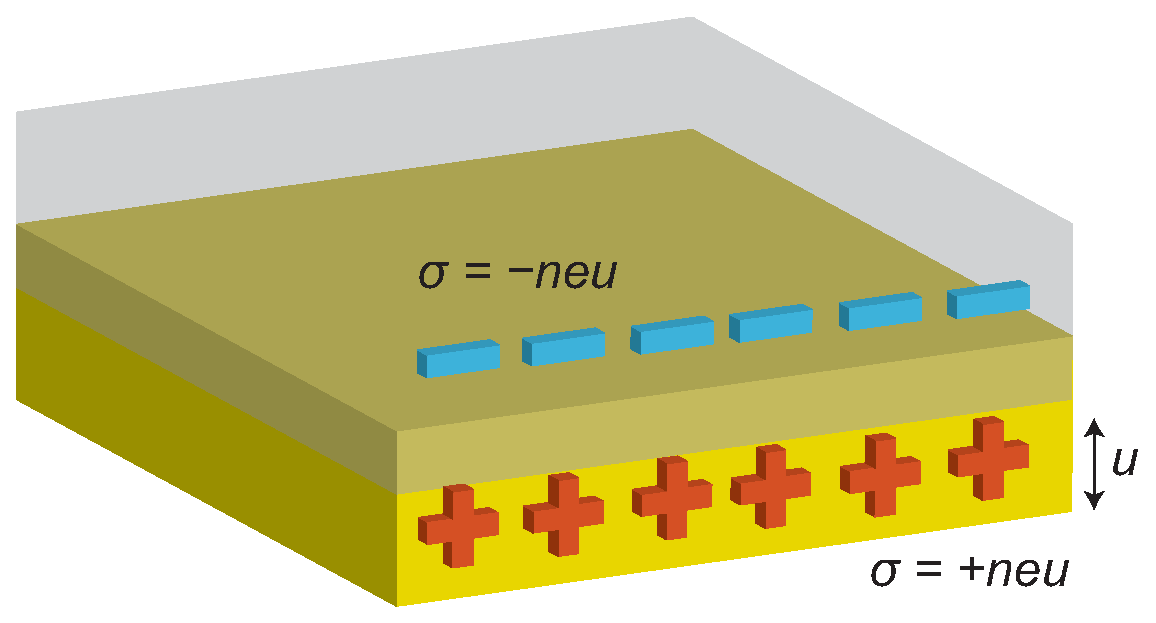
\includegraphics[scale=0.5]{THM/bulk.eps}
\caption{\label{fig:bulk}Longitudinal collective oscillations of the conduction electrons of a metal (Volume plasmons)}
\end{figure}
 We can derive plasma frequency $\omega_p$ from the simple harmonics oscillation model, a collective displacement of the electron cloud by a distance $u$ leads to a surface charge density $\sigma = \pm neu$ at the slab boundaries. This establishes a homogeneous electric field $\mathbf{E} = \frac{neu}{\varepsilon_0}$ inside the slab. Thus, the displaced electrons experience a restoring force, and their movement can be described by the equation of motion $nm\ddot{u} = -ne\mathbf{E}$. Inserting the expression for the electric field, this leads to
 \begin{subequations}
 \begin{align}
 nm\ddot{u} = -\frac{n^2e^2u}{\varepsilon_0} \\
 \ddot{u} + {\omega_p}^{2}u = 0\text{.}
 \end{align}
 \end{subequations}
  The plasma frequency $\omega_p = \sqrt{\frac{ne^2}{\varepsilon_0m}}$ can thus be recognized as the natural frequency of a free oscillation of the electron sea. The quanta of these charge oscillations are called plasmons. Due to the longitudinal nature of the excitation, volume plasmons do not couple to transverse electromagnetic waves, and can only be excited by particle impact. We can derive the dispersion relation of the generalization of volume plasmons, traveling plasma waves, from curl electric field equations (Equations~\ref{eq:curlE})
 \begin{subequations}
 \begin{align}
 \curl{\curl \mathbf{E}} &= -\mu_0 \frac{\partial^2\mathbf{D}}{\partial t^2}\label{eq:curlE}\\
\mathbf{K}( \mathbf{K}\cdot \mathbf{E}-K^{ 2 }\mathbf{E} ) &=-\varepsilon ( \mathbf{K},\omega  ) \frac { { \omega  }^{ 2 } }{ { c }^{ 2 } } \mathbf{E}
 \end{align}
 \end{subequations}  
and plasma model, and a simple equation of motion for an electron of the plasma subjected to an external electric field $\mathbf{E}$
 \begin{equation}
m\ddot{\mathbf{x}} + m\gamma\dot{\mathbf{x}} = -e\mathbf{E}\text{.}
\end{equation}
Assuming a harmonic time dependence $\mathbf{E}( t )=\mathbf{E}_0\mathrm{e}^{-i\omega t}$ of the driving field, a particular solution of this equation describing the oscillation of the electron is $\mathbf{x} ( t ) = \mathbf{x}_0 \mathrm{e}^{-i\omega t} $. The complex amplitude $\mathbf{x}_0$ incorporates any phase shifts between driving field and response via
\begin{equation}
\mathbf{x} ( t ) = \frac{e}{m( \omega^2 + i\gamma\omega )}\mathbf{E}( t )\text{.}
\end{equation}
The displaced electrons contribute to the macroscopic polarization
\begin{equation}
\mathbf{P}=-\frac{ne^2}{m( \omega^2 + i\gamma\omega )}\mathbf{E}( t )\text{.}
\end{equation}
Inserting $\mathbf{P}$ into dielectric displacement field equation $\mathbf{D} = \varepsilon_0\mathbf{E} + \mathbf{P}$ yields
\begin{equation}
\mathbf{D} = \varepsilon_0(1-\frac{\omega_p^2}{\omega^2 + i\gamma\omega})\mathbf{E}\text{,}
\end{equation}
where $\omega_p^2 = \frac{ne^2}{\varepsilon_0m}$. Therefore, the dielectric function of the free electron gas
\begin{equation}
\varepsilon(\omega) = 1- \frac{\omega_p^2}{\omega^2 + i\gamma\omega}\text{.}\label{eq:dielefu}
\end{equation}
We arrive at the desired result by using equation~\ref{eq:dielefu} and the generic dispersion relation $K^2=\varepsilon(\mathbf{K},\omega)\frac{\omega^2}{c^2}$, the dispersion relation of traveling waves becomes
\begin{equation}
\omega^2 = \omega_p^2 + \mathbf{K}^2c^2\text{.}
\end{equation}
From this relation, we can figure out the oscillation properties in any frequency of external field. Note that this branch can not confine the electromagnetic waves, it would radiate out the energy, so this mode is also called radiative surface plasmon.

\section{Surface plasmon polaritons at interface between dielectric and metal}

Surface plasmon polaritons (SPPs) are eigenmodes of transverse magnetic (TM) waves, which coupling the electromagnetic fields to oscillations of the conductor's electron plasma, propagate at a interface between dielectric and metal, and are confined in perpendicular direction. Providing a flat interface between dielectric and metal half-spaces with dielectric constants $\varepsilon_d$ and $\varepsilon_m$ , respectively, and assuming the interface normal to z direction and the SPPs propagate along the $x$ direction, the SPP wave vector $\beta$ is related to the frequency $\omega$ through the dispersion relation
\begin{equation}
\beta = k_0\sqrt{\frac{\varepsilon_d\varepsilon_m}{\varepsilon_d + \varepsilon_m}}\text{,}\label{eq:sppsdisp}
\end{equation}
where $k_0 = \omega/c$ is the free-space wave vector. We take $\omega$ to be real and allow $\beta$ to be complex.

The optical response of metals is often described by the Drude model for a free-electron gas~\cite{kittel1976introduction},
\begin{equation}
\varepsilon_{Drude}(\omega)=1-\frac{\omega_p^2}{\omega^2+i\Gamma\omega}\text{,}
\end{equation}
in which $\Gamma$ is a damping rate due to electron-electron and electron-phonon scattering.
Figure~\ref{fig:SPPdisp} shows the dispersion curve~\ref{eq:sppsdisp} with Drude metal  in the absence of losses ($\Gamma=0$) for air ($\varepsilon_d = 1$) and fused silica ($\varepsilon_d = 2.25$) interface.
\begin{figure}[htb]
\centering
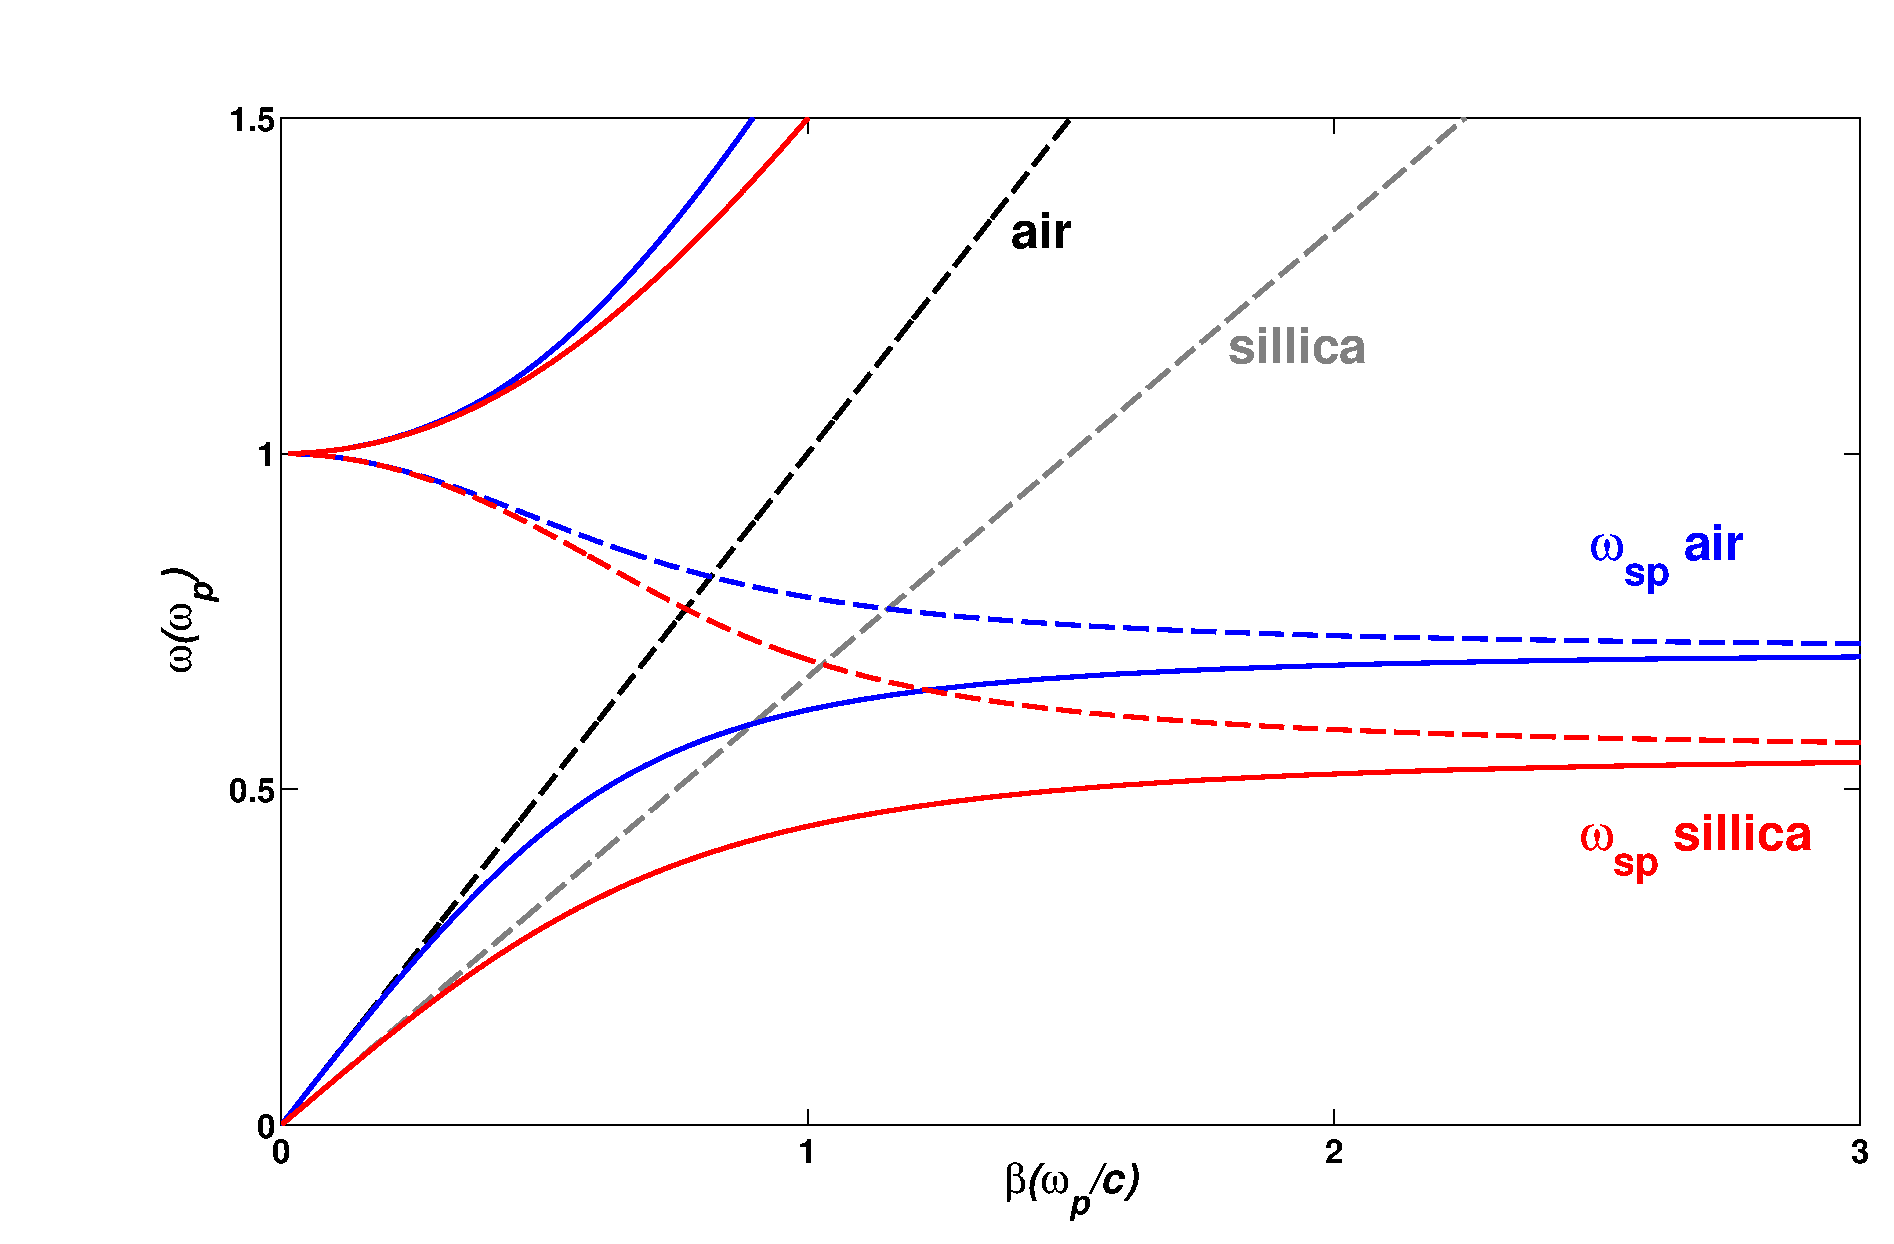
\includegraphics[scale=0.4]{THM/SPPdisp.eps}
\caption{\label{fig:SPPdisp}Dispersion relation of SPPs at the interface between a Drude metal with negligible collision frequency and air (blue curves) and silica (red curves).}
\end{figure}
For small wave vectors SPPs propagation constant $\beta$ is close to $k_0$ at the light line, in the opposite regime of the frequency close to surface plasmon frequency $\omega_p$. It also shows that the SPPs line lying to the right of the respective light lines of air and silica, so that SPPs are directed by light due to phase mismatching. The wave vector mismatch between SPPs and radiation modes needs to be overcome in order to excite or detect SPPs. This can be achieved by multiple methods~\cite{raether1988surface}. In the Otto configuration, light in a prism that is brought in close vicinity to a metal surface can excite SPPs through coupling to the evanescent field. Because light in the prism has a larger wave vector than that in air, it can be phase-matched to the SPPs. In the related Kretschmann-Raether geometry, coupling to SPPs occurs through a metal film that is deposited on a prism. In the grating coupling configuration, metal surface with a shallow grating of grooves or holes with lattice constant $a$. For the simple 1D grating of grooves depicted in Figure~\ref{fig:grating},
\begin{figure}[htb]
\centering
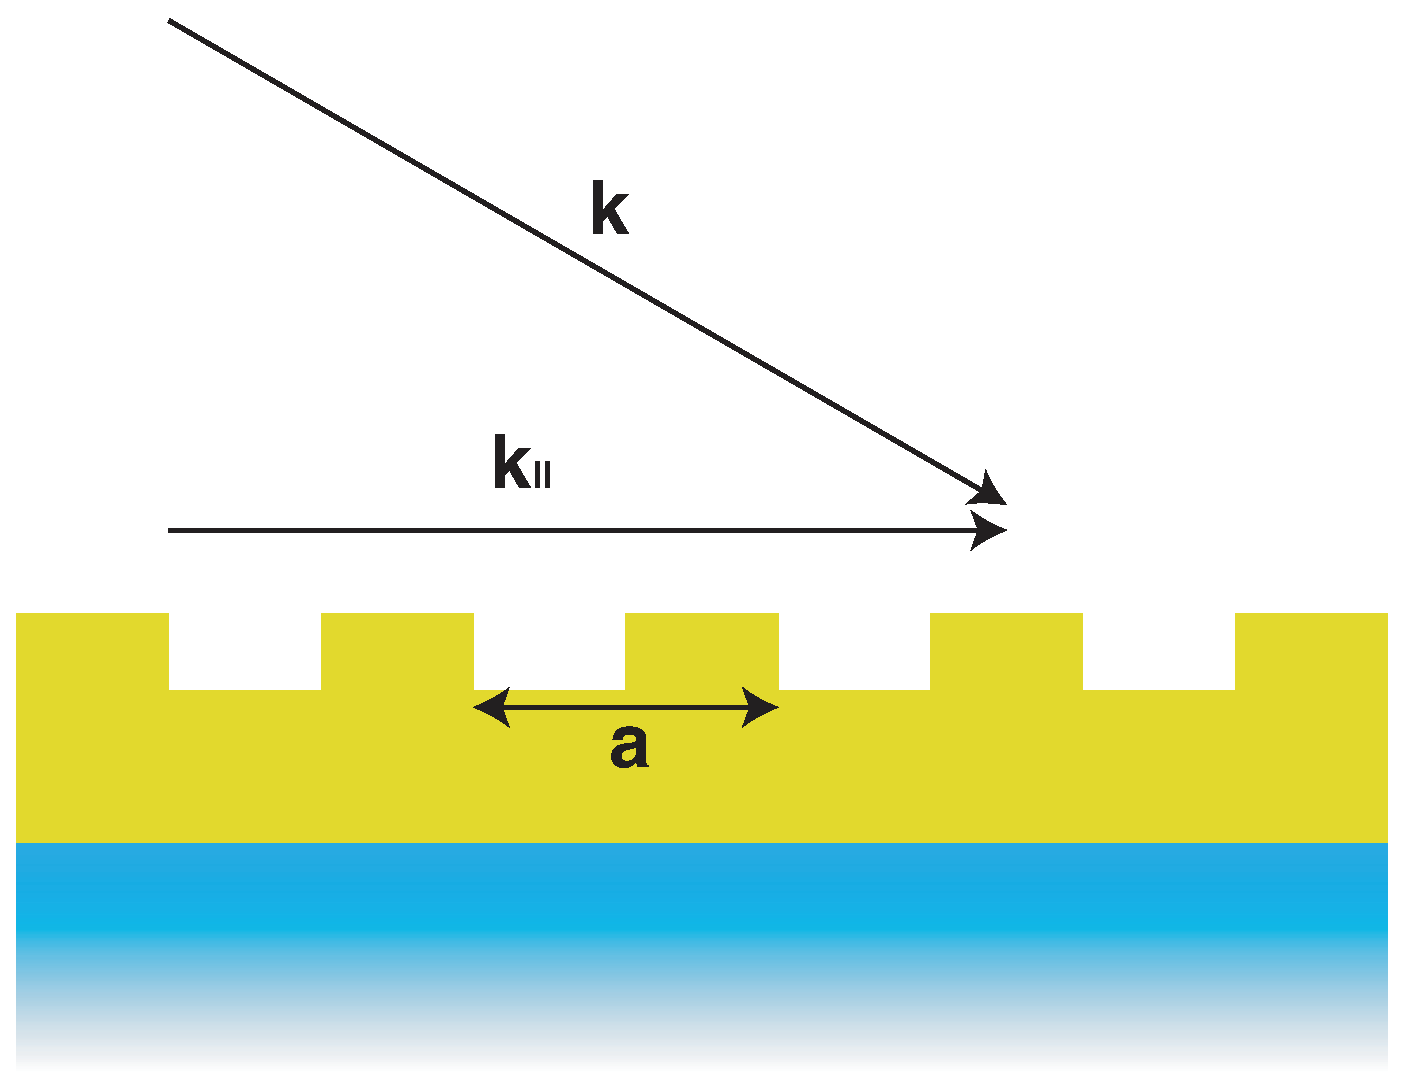
\includegraphics[scale=0.5]{THM/grating.eps}
\caption{\label{fig:grating}Phase-matching of light to SPPs the grating coupling configuration.}
\end{figure}
phase-matching takes place when the condition is fulfilled
\begin{equation}
\beta = k_0 \sin{\theta} \pm \nu g\text{,}
\end{equation}
where $g=\frac{2\pi}{a}$ is the reciprocal vector of the grating, and $\nu=(1,2,3\dots)$.
As with prism coupling, excitation of SPPs is detected as a minimum in the reflected light. The reverse process can also take place, SPPs propagating along a surface modulated with a grating can couple to light and thus radiate. 

%\bibliographystyle{unsrt}
%\bibliography{thesisbib} %old
%\chapter{Experiment}
\label{c:exp}

\section{Experiment Setup} % (fold)
\label{s:experiment_setup}

In this section, we discuss the resluts of our experiments.  There are four parts in our experiments.  First, we compare our framework with other frameworks in the communication cost.  Second, since there are several stages of improvement in our framework, we discuss each of their influence to our final model.  Third, we consider the amortization of transmitting the orthogonal matrices.  Finally, we compare the power of pruning among different bounds.  For every experiment, we collect the results of $100$ experiments by randomly picking our $100$ instances as the queries.
% section experiment_setup (end)

\section{Data Description} % (fold)
\label{s:data_description}

The table \ref{table:datasets} is the description of those datasets we used in our experiments. Note that the $n\times m$ in the final column means that there are $n$ instances placed in each machine and $m$ machines used in this experiments.  For instance, for the image dataset ANN with SIFT feature, there are totally $5000$ machines and each has $200$ instances in our experiments.

\begin{table}[htpb]\begin{center}
\caption{Summary for each dataset}\label{table:datasets}
\begin{tabular}{|c|c|c|c|c|}
\hline 
Type & Dataset & Feature & Num of Dimensions & Num of Instances\\ \hline \hline
Time Series & Random Walk & $N(0,1)$ & 128 & $200\times 5000$\\ \hline
\multirow{3}{*}{Image} & ANN & SIFT & 128 & $200\times 5000$\\ 
\cline{2-5}
 & \multirow{2}{*}{Flickr} & CSD & 256 & $500\times 2000$\\ 
\cline{3-5}
 & & SCD & 256 & $500\times 2000$\\ \hline
 \multirow{2}{*}{Audio} & \multirow{2}{*}{Million Songs} & MVD & 480 & $500\times 1900$ \\ 
 \cline{3-5}
 & & TRH & 480 & $500\times 1900$\\ \hline
\end{tabular}
\end{center}\end{table}

\subsection{Time Series Data} % (fold)
\label{ssb:time}
The time series datasets we used is a synthetic dataset.  We use the random walk data model in \cite{time}.  Each time series is generated by a random walk whose every step size is a normal distributed random number with mean $0$ and standard deviation $1$.  We also use this model to generate the synthetic dataset in the experiments of MsWave \cite{MsWave}.
% subsection time (end)

\subsection{Image Data} % (fold)
\label{ss:Image}
We use two datasets in our experiments for images.  First is the data provied in \cite{ANN}, which is a widely used dataset for evaluate the performance of approximate nearest neighbors search algorithms.  The another one is the Flickr datasets with two kind of features used in \cite{Flickr}.  The dataset is also a widely used dataset in the task of image retrieval.  The CSD indicates \emph{Color Structure Descriptor} while the SCD means \emph{Scalable Color Descriptor}.
% subsection Image (end)

\subsection{Audio Data} % (fold)
\label{sub:audio_data}
Here we use the audio data named Million Song Dataset from~\cite{Bertin-Mahieux2011} which is a free-available collection of audio features for a million contemporary popular music tracks. For the features, MVD means \emph{Modulation Frequency Variance Descriptor} and TRH is \emph{Temporal Rhythm Histograms}.  Please refer to \cite{LID_05ismir,RAU_03jnmr,RAU_01ecdl} to see the details about how these features were extracted.
% subsection audio_data (end)

% subsection data_description (end)

\section{Comparison Among all Frameworks} % (fold)
\label{s:comparison_among_all_frameworks}

\subsection{Frameworks for Comparison} % (fold)
\label{ss:frameworks_for_comparison}

We compare our framework with those methods mentioned in the related work chapter.  From \cite{PRP}, we use CP and PRP but with slightly modifications. In the origin CP, every machine would return the top $k$ instances once receiving the query.  But there is a trivial improvement that every machine only return the \emph{distances} of these top $k$ instances.  Then, the server could know the distances of the $k$NN of this query and then ask those machines with answers to return those instances.  Although it is a slight modification, it could reduce the cost of CP a lot when the number of machines is large.  Also, we run LeeWave \cite{LeeWave} in these experiments for comparision.  We call our final framework as \emph{Main} in the following figures.


Note that in the following experiments, the cost of our framework here does not include the cost of sending the orthogonal matrices.  We will prove in the section~\ref{s:number_of_queries_for_amortizing_the_cost_of_matrices} that the total cost including the matrices could be amortized by enough queries and thus to achieve the cost here.  That is, we could see the cost of our framework here as the cost after amortized by enough queries.  Due to the time limitations, we didn't conduct enough number of queries to achieve the amortized results for each dataset.


% subsection frameworks_for_comparison (end)

\subsection{Results of Different Frameworks} % (fold)
\label{sub:results_of_different_fra}

The following figures are the results of our experiments.  The $x$ axis indicates the number of local machines while the $y$ axis is the total transmission cost of the 100 queries.  Since the differences among these are too large, we transform the $y$ axis to logarithmic scale.  

\begin{figure}[htpb!]
  \centering
  \includegraphics[width=1.0\linewidth]{exp/out/time.png}
  \caption{Different Frameworks on Time Series}
  \label{fig:out_time}
\end{figure}

\begin{figure}[htpb!]
  \centering
  \includegraphics[width=1.0\linewidth]{exp/out/ANN.png}
  \caption{Different Frameworks on ANN}
  \label{fig:out_ANN}
\end{figure}

\begin{figure}[htpb!]
  \centering
  \includegraphics[width=1.0\linewidth]{exp/out/f2.png}
  \caption{Different Frameworks on Flickr:~CSD}
  \label{fig:out_f2}
\end{figure}

\begin{figure}[htpb!]
  \centering
  \includegraphics[width=1.0\linewidth]{exp/out/f3.png}
  \caption{Different Frameworks on Flickr:~SCD}
  \label{fig:out_f3}
\end{figure}

\begin{figure}[htpb!]
  \centering
  \includegraphics[width=1.0\linewidth]{exp/out/mvd.png}
  \caption{Different Frameworks on Million Song:~MVD}
  \label{fig:out_mvd}
\end{figure}

\begin{figure}[htpb!]
  \centering
  \includegraphics[width=1.0\linewidth]{exp/out/trh.png}
  \caption{Different Frameworks on Million Song:~TRH}
  \label{fig:out_trh}
\end{figure}

From these figures, we could see that our framework used the least transmission cost among all these frameworks for every dataset.  And these differences between our framework and each other framework increased as the number of local machines increased.  The reason is that when the number of local machines increases, there would be a higher chance to prune more local machines in the early round since the ratio of pruned machines doesn't change too much.  But the other frameworks would be more sensitive to the number of local machines.


The performance of CP and PRP are similar to each other in most dataset.  It is because when $k$ is much smaller than the number of total local machines, their procedure would be almost the same except the final stage.  For those cases where PRP is worse than CP, we could find that PRP would return too many instances in the final stage while CP would only return exact $k$ instances back to the server.  But these results would highly depend on the distribution of the instances among these local machines and could not be controled by the algorithms themself.


We could also notice that LeeWave needs the largest transmission cost to finding the $k$NN for the $100$ queries for all datasets.  When the type of the dataset is time series (figure \ref{fig:out_time}), the different between LeeWave and other frameworks are smaller than other datasets since its pruning power is still effective for this type of dataset. For other types of datasets like images or audio, LeeWave almost could not prune any candidiate machines until the last round which would sent the whole query to each machine and thus used a large amount of transmission cost. 

Even though the LeeWave could prune some candidates machines when the type of the dataset is time series, there is a big gap between it and CP, PRP.  The reason of the large transmission cost in LeeWave here is not the pruning power but its way to calculate the bounds.  In each round, after sending the coefficients in this level of the error tree, LeeWave requires every instances to return some metadata back for calculating the bounds at the server.  This causes one term in the transmission cost of LeeWave would grows linearly with the total number of instances in all local machines.  Since we conducted our experiments on the datasets with about one million instances, this term would be large enough to cover the saving from the pruning.  On the other hand, the transmission cost of CP and PRP is independent of the total number of instance but only dependent on the number of local machines and $k$.  Therefore, when the total instances is large, LeeWave could use more transmission cost than CP and PRP even when its pruning power still exists.


% subsection results_of_different_fra (end)	
% section comparison_among_all_frameworks (end)



\section{Comparison Among our Framework with Different Configurations} % (fold)
\label{s:comparison_among_our_framework_with_different_configurations}


\subsection{Configurations for Comparison} % (fold)
\label{sub:configurations_for_comparison}

There are many stages of algorithms which build the final version of our framework.  Therefore, in this section, we would like to discuss the performance of our framwork with or without each of these algorithms.  We conducted the experiments for the following different configurations of our framework.

\emph{Main}: It is the final version of our framework which obtains all algorithms mentioned in the chapter of methodology.

\emph{NoW}: To test the influence of the orthogonal transformation, we consider the configuration which has all the algorithms except the orthogonal transmission.  We could take it as the special case of \emph{Main} where $W_i=I,~\forall i=1,2,\ldots,m$.

\emph{NoPRP}: In the section~\ref{ss:find_the_threshold_in_distributed_machines}, we use PRP to find the threshold for pruning in each round.  Therefore, we want to compare this modification with the original version which directly returns all bounds back to the server.

\emph{NoCD}: In the section~\ref{ss:coordinate_descent_to_decide_the_pivots}, the number of dimensions we sent for every query are decided dynamically by solving an optimization problem with Coordinate Descent.  Here we just send $10\%$ of the transformed query in each round to the server for comparing the improvement from the optimiaztion.

% subsection configurations_for_comparison (end)

\subsection{Results of Different Configurations} % (fold)
\label{sub:results_of_different_configurations}


We provide the results of the experiments to compare our framework with different configurations in the following figures. The meanings of their axises are same with those in the section \ref{sub:results_of_different_fra}.

\begin{figure}[htpb!]
  \centering
  \includegraphics[width=1.0\linewidth]{exp/in/time.png}
  \caption{Different Configurations on Time Series}
  \label{fig:in_time}
\end{figure}

\begin{figure}[htpb!]
  \centering
  \includegraphics[width=1.0\linewidth]{exp/in/ANN.png}
  \caption{Different Configurations on ANN}
  \label{fig:in_ANN}
\end{figure}

\begin{figure}[htpb!]
  \centering
  \includegraphics[width=1.0\linewidth]{exp/in/f2.png}
  \caption{Different Configurations on Flickr:~CSD}
  \label{fig:in_f2}
\end{figure}

\begin{figure}[htpb!]
  \centering
  \includegraphics[width=1.0\linewidth]{exp/in/f3.png}
  \caption{Different Configurations on Flickr:~SCD}
  \label{fig:in_f3}
\end{figure}

\begin{figure}[htpb!]
  \centering
  \includegraphics[width=1.0\linewidth]{exp/in/mvd.png}
  \caption{Different Configurations on Million Song:~MVD}
  \label{fig:in_mvd}
\end{figure}

\begin{figure}[htpb!]
  \centering
  \includegraphics[width=1.0\linewidth]{exp/in/trh.png}
  \caption{Different Configurations on Million Song:~TRH}
  \label{fig:in_trh}
\end{figure}

In these figures, we could see that although every algorithm could make our framework better, their influences are very different to each other.  The algorithm which makes the largest difference with our final framework is PRP.  It is very obvious since we use PRP to find the threshold could make the transmission cost independent with the total number of instances.  This makes a big difference when the datasets here contain about one million instances.  The algortihm with the second big improvement is the orthogonal transformation.  This confirms our assumption that we could save transmission cost by improving the power of pruning with the help of the orthogonal transformation.  Finally, the algorithm of dynamically deciding the pivots with Coordinate Descent seems to have the least influence to our final framework in these figures.  However, it does contibute much to the saving of transmission even though not as significant as the others.  With the help of it, we don't have to worry about deciding the pivots for every dataset.

% subsection results_of_different_configurations (end)
% section configurations_for_comparison (end)

\section{Number of Queries for Amortizing the Cost of Matrices} % (fold)
\label{s:number_of_queries_for_amortizing_the_cost_of_matrices}

In the beginning of this chapter, we mentioned that the cost of our final framework showed in the previous experiments didn't count the cost of sending those orthogonal martices.  The matrices cost from the first phase of our framework is as below. 
\begin{equation}
\begin{aligned}
	Cost_{Matrix} & = m\times SingleMatrixCost \\
                  & = m\times \frac{D\times (D-1)}{2}
\end{aligned}
\end{equation}

where we have given the proof that we could use $\frac{D\times (D-1)}{2}$ parameters to represent an orthogonal matrix in the section \ref{ss:reduce_the_cost_of_sending_matrices}.


Although it would cause a large cost, it only needs to be done for one time.  Therefore, we could amortize it to the cost of every query in the second phase.  If the number of queries is large enough, we could amortize the matrices cost to a very small ratio of the total transmission cost.  But due to the time limitation, we didn't conduct the experiments for a large number of queries, therefore, we estimate the number of queries we need as below.

Given a small ratio (here we use $r_{ideal}=5\%$), we could estimate how many queries we need for amortizing the matrices cost to this ratio of the total transmission cost as below.  

\begin{equation}
\begin{aligned}
	Cost_{Total} & = & \sum_{t=1}^{\Vert Q\Vert}{Cost_{our}(q_t)} + Cost_{Matrix} \\
	Cost(i) & = & \frac{\sum_{t=1}^{\Vert Q\Vert}{Cost_{our}(q_t)}}{{\Vert Q\Vert}}\times i + Cost_{Matrix} \\
\end{aligned}
\end{equation}

In the equation above, we estimate the total cost of $i$ queries as $Cost_(i)$ by summing up the matrices cost and the average cost of the second phase in our past experiments multiplied by $i$.  In other words, we estimate the cost of the second phase for a single query as $\frac{\sum_{t=1}^{\Vert Q\Vert}{Cost_{our}(q_t)}}{{\Vert Q\Vert}}$. 

Therefore, our goal becomes how many queries we need to make the ratio of $Cost_{Matrix}$ lower than $r_{ideal}$.  We could write it as the following problem:

\begin{equation}\label{eq:amort}
\begin{aligned}
& \underset{i}{\text{minimize}}
~~\frac{Cost_{Matrix}}{Cost(i)} < r_{ideal} \\
& \text{where}~~i \in \mathbb{N}
\end{aligned}
\end{equation}

It could be solved easily.


\begin{table}[H]\begin{center}
\caption{Number of queries to amortize the cost of matrices}\label{table:amortize}
\begin{tabular}{|c|c|c|c|c|c|}
\hline 
Type & Dataset & Feature & Total Num of Instances & Num of Queries\\ \hline \hline
Time Series & Random Walk & $N(0,1)$ & $1000000$ & $4655$\\ \hline
\multirow{3}{*}{Image} & ANN & SIFT & $1000000$ & $1997$\\ 
\cline{2-5}
 & \multirow{2}{*}{Flickr} & CSD & $1000000$ & $6313$\\ 
 \cline{3-5}
 & & SCD &  $1000000$ & $12724$\\ \hline
 \multirow{2}{*}{Audio} & \multirow{2}{*}{Million Songs} & MVD & $950000$ & $6979$\\ 
 \cline{3-5}
 & & TRH & $950000$ & $7076$\\ \hline
\end{tabular}
\end{center}\end{table}

We solve~\eqref{eq:amort} for each dataset when the number of local machines reachs the maximal and $k=10$.  The results are put in the table \ref{table:amortize}.  From this table, we could find that although the matrices cost is large, we could amortize it to less than $5\%$ with a few thousands of queries.  For a dataset with one million of instances, the number of queries could be achieved easily.  


\begin{figure}[htpb!]
  \centering
  \includegraphics[width=1.0\linewidth]{exp/AQ/ANN.png}
  \caption{Pruning Results on Time Series}
  \label{fig:AQ}
\end{figure}

From the figure~\ref{fig:AQ}, we could notice that $\frac{Cost_{Matrix}}{Cost(i)} < r_{ideal}$ decreases fast as the number of queries increases.  As our estimation, this ratio achieve $5\%$ when the number of queries reach about $2000$.




% subsection number_of_queries_for_amortizing_the_cost_of_matrices (end)



\section{Power of the Pruning Procedure} % (fold)
\label{s:power_of_the_pruning_procedure}

\subsection{Methods with Different Bounds} % (fold)
\label{sub:methods_with_different_bounds}


There are three different bounds which we could compare.  The first one is the bounds of LeeWave, which comes from the Haar wavelet transformation.  The second one is the bounds we derived in the section~\ref{ss:derivation_of_the_bounds}.  That is the method \emph{NoW} we mentioned above.  The final bounds is those improved by the orthogonal transformation.


% subsection methods_with_different_bounds (end)


\subsection{Results of Pruning} % (fold)
\label{sub:results_of_pruning}

First, we compare the bounds we derived and the bounds of LeeWave.  Since the number of dimensions LeeWave sent in every round is restricted by the shape of the error tree, we could only compare the number of residual machines under these dimensions between LeeWave and our method.  For LeeWave, we just average the results of each query.  As for our method, we use our estimation for each dimension used in the section~\ref{ss:estimate_the_number_of_residual_machines} and pick those dimesions used in LeeWave.

From the table~\ref{table:time} for time series dataset, we could see that although LeeWave could prune some local machines in the last few round, our method outperforms it by pruning machines earlier and more.  This improvement mainly comes from our tighter bounds that provide a more powerful pruning mechanism.

\begin{table}[H]\begin{center}
\caption{Time Series, Number of residual machines after sending some dimensions for 5000 machines}\label{table:time}
\begin{tabular}{|c|c|c|c|c|c|c|c|c|}
\hline 
Method \textbackslash Dim & 2 & 4 & 8 & 16 & 32 & 64 & 128\\ \hline \hline
Ours & 4823.24 & 4469.71 & 3762.66 & 2344.46 & 540.14 & 69.11 & 9.99 \\ \hline
LeeWave & 4999.84 & 4984.90 & 4895.18 & 3722.49 & 938.80 & 111.00 & 9.99 \\ \hline
\end{tabular}
\end{center}\end{table}

However, for the other types of datasets, from these tables we could notice that LeeWave almost could not prune any local machine until the last round.  The reason is that since the bounds of LeeWave come from the Haar wavelet transformation, which is suitable for the time series feature, but not workable for the images and audio datasets from these experiments.  Although the power of pruning of our method would be different for different types of data, we could prune about half of total local machines after sending half of the query feature vector.  This allows us to avoid sending redundant information to unnecessary machines.


\begin{table}[H]\begin{center}
\caption{Flickr:CSD, Number of residual machines after sending some dimensions for 1000 machines}\label{table:f2}
\begin{tabular}{|c|c|c|c|c|c|c|c|c|c|}
\hline 
Method \textbackslash Dim & 2 & 4 & 8 & 16 & 32 & 64 & 128 & 256\\ \hline \hline
Ours & 995.37 & 986.10 & 967.56 & 930.49 & 856.34 & 573.79 & 410.3 & 9.89 \\ \hline
LeeWave & 1000 & 1000 & 1000 & 999.90 & 995.16 & 967.26 & 808.16 & 9.89 \\ \hline
\end{tabular}
\end{center}\end{table}


\begin{table}[H]\begin{center}
\caption{Million Songs: MVD, Number of residual machines after sending some dimensions for 800 machines}\label{table:mvd}
\begin{tabular}{|c|c|c|c|c|c|c|c|c|c|}
\hline 
Method \textbackslash Dim & 2 & 6 & 12 & 26 & 52 & 104 & 210 & 420\\ \hline \hline
Ours & 799.41 & 797.05 & 793.5 & 785.23 & 769.87 & 739.14 & 467.74 & 12.77 \\ \hline
LeeWave & 800 & 800 & 800 & 800 & 799.07 & 794.93 & 772.91 & 12.58 \\ \hline
\end{tabular}
\end{center}\end{table}


Finally, let's discuss the pruning power with or without the help of the orthogonal transformation, which is our final method and \emph{NoW}.  We plot our estimation in the section~\ref{ss:estimate_the_number_of_residual_machines} and compare their estimation.  However, we found that for some datasets, these could not reflect the status of pruning for \emph{NoW} since the decision of the pivots are concentrated in the latter part of the vector.  As a result, we add another method named \emph{NoCDW} which is same with \emph{NoW} but intead of dynamically deciding the pivots, it sends $10\%$ of the vector for each round.  In the following figures, the red circles are our final method, the black ones are \emph{NoW}, and the green ones are \emph{NoCDW}.

From the figure~\ref{fig:prune_ANN} and figure~\ref{fig:prune_trh}

For all these figures except the figure~\ref{fig:prune_f3}, we could see that our method could prune most of the residual machines with about $50\%$ of the total dimensions.  From \emph{NoCDW}, we could find we have to send many dimensions to prune some machines without the orthogonal transformation.  This difference comes from the tightness of the bounds.  After optimizing with the orthogonal transformation, our method could use much tighter bounds to prune machines than the original bounds.  With the enhanced prunine power, our method could save much transmission cost.

On the other hand, in the figure~\ref{fig:prune_ANN} and figure~\ref{fig:prune_trh}, the curve of \emph{NoW} is very different with \emph{NoCDW}.  The reason is that for these datasets, the pivots learnt from the estimation cost problem concentrate at the latter part of the vector, which leads to very poor estimation for residual machines for the earlier part of the vector.  So, its curve could not reflect the pruning power of the bounds without transformation.  This also implies the policy of sending $10\%$ total dimensions would not be the best policy for these datasets since the curve of \emph{NoW} is mcuh different with the one of \emph{NoCDW}.  For the other figures, we could see the curve of \emph{NoW} is similar with \emph{NoCDW}. This implies the $10\%$ policy would be fine for these datasets.  But since we could not know whether this policy would work for a dataset in advance, the best policy is to decide the pivots dynamically as we mentioned before.

\begin{figure}[htpb!]
  \centering
  \includegraphics[width=1.0\linewidth]{exp/prune/ANN.png}
  \caption{Pruning Results on ANN}
  \label{fig:prune_ANN}
\end{figure}

\begin{figure}[htpb!]
  \centering
  \includegraphics[width=1.0\linewidth]{exp/prune/f2.png}
  \caption{Pruning Results on Flickr:~CSD}
  \label{fig:prune_f2}
\end{figure}

\begin{figure}[htpb!]
  \centering
  \includegraphics[width=1.0\linewidth]{exp/prune/f3.png}
  \caption{Pruning Results on Flickr:~SCD}
  \label{fig:prune_f3}
\end{figure}

\begin{figure}[htpb!]
  \centering
  \includegraphics[width=1.0\linewidth]{exp/prune/mvd.png}
  \caption{Pruning Results on Million Song:~MVD}
  \label{fig:prune_mvd}
\end{figure}

\begin{figure}[htpb!]
  \centering
  \includegraphics[width=1.0\linewidth]{exp/prune/trh.png}
  \caption{Pruning Results on Million Song:~TRH}
  \label{fig:prune_trh}
\end{figure}


% subsection results_of_pruning (end)	


% section power_of_the_pruning_procedure (end)

%\bibliographystyle{unsrt}
%\bibliography{thesisbib} %old
%\include{main} %old
%\chapter{Conclusions}
\label{c:conclusions}

Distributed similarity search becomes increasingly crucial as there are various types of datasets on the mobile devices today.  However, we need to deal with the huge transmisson cost while searching the answers among these distributed machines.  In this paper, we propose a two-phase framework which is able to use much less transmission cost to find our desired answers with the help of the orthogonal transformation.  We conducted experiments on various types of datasets to confirm the generalization of our framework.  From the results of these experiments, we could see that our framework could maintain its performance while facing very different kinds of data.

From our framework, we could find that there are many useful properties of orthogonal transformation, especially the property to preserve the distance relationship.  As long as we could design a reasonalbe objective function of the transformation and optimize it well, it is possible to make those values which are unchangeable in the original space become functions of the transformation in the transformed space while preserving many properties in the original space.

Although our framework outperforms other frameworks in the experiments, there are some directions which could further improve our framework.  

First, the transmission cost of the first phase is still too much.  If we could reduce the matrices cost more, we could use less queries to amortize this cost.  We could compress these matrices and thus send them with less transmission cost.  After the server receives these matrices, they could be reconstructed back to orthogonal matrices by SVD.  However, the compression might be lossy.  And it would become a tradeoff between the performance of pruning and the transmission cost.

The another direction would be the estimation of the transmission cost before sending a query.  Before estimating this cost, we have to estimate the number of residual machines like we mentioned in the section ~\ref{ss:estimate_the_number_of_residual_machines}.  In this paper, we use a simple linear interpolation to estimate those dimensions with empty value.  If we could estimate them more precisely, we could get a better pivots to send the query.

Since our framework are comprised of several individual subproblems, its overall performance could be improved as long as any of the subproblem is solved by a better alorithm. %old


\appendix
%----------- Input your appendix here  -----------
%\chapter{First appendix title}

Open and edit \href{run:./AppendixA.tex}{AppendixA.tex} 
%or %chapter cite  == \include
%\chapter{First appendix title}

Open and edit \href{run:./AppendixA.tex}{AppendixA.tex}

\backmatter


%---------- Input your reference here ---------
\bibliographystyle{unsrt}
\addcontentsline{toc}{chapter}{\bibname}
\bibliography{r44}
%\bibliography{thesisbib}

%----------- Input your Figure chapter here  -----------
%\chapter*{}  %加星號隱藏標題

%----------- 重新設定counter格式,章節圖檔和表格的計數器格式皆為1…9 -----------
\renewcommand{\thefigure}{\arabic{chapter}.\arabic{figure}} 
\renewcommand{\thetable}{\arabic{chapter}.\arabic{table}} 
%--------- Input your main figures and tables here  ---------
\setcounter{chapter}{3}%使章節couter切回3,第三章圖放在此行之後
\setcounter{figure}{1}  %使圖檔couter切回1
\setcounter{table}{1}  %使表格couter切回1

\begin{figure}[!]
\centering
\includegraphics[scale=0.5]{THM/bulk.eps}
\caption{\label{fig:bulk}Longitudinal collective oscillations of the conduction electrons of a metal (Volume plasmons)}
\end{figure}

\begin{table}[!]\begin{center}
\caption{Table Example 1}
\begin{tabularx}{8cm}{llX}
\hline
Start & End  & Character Block Name \\
\hline
3400  & 4DB5 & CJK Unified Ideographs Extension A \\
4E00  & 9FFF & CJK Unified Ideographs \\
\hline
\end{tabularx}
 \end{center}\end{table}
 
\begin{figure}[!]
\centering
\includegraphics[scale=0.4]{THM/SPPdisp.eps}
\caption{\label{fig:SPPdisp}Dispersion relation of SPPs at the interface between a Drude metal with negligible collision frequency and air (blue curves) and silica (red curves).}
\end{figure}

\setcounter{chapter}{4}  %使章節couter切回4,第4章圖放在此行之後
\setcounter{figure}{1}  %使圖檔couter切回1

\begin{figure}[!]
\centering
\includegraphics[scale=0.35]{EXP/afm1.eps}
\caption{\label{fig:afm1}Schematic of atomic force microscopy.}
\end{figure}

\begin{figure}[!]
\centering
\includegraphics[scale=0.6]{EXP/afm3.eps}
\caption{\label{fig:afm3}Sketch of tip-sample forces.}
\end{figure}

%----------- 重新設定counter格式,章節的計數器格式為A…Z,圖檔和表格的格式皆為1…9 -----------
\renewcommand{\thefigure}{\Alph{chapter}.\arabic{figure}} 
\renewcommand{\thetable}{\Alph{chapter}.\arabic{table}}
%--------- Input your appendix figures and tables here  ---------
\setcounter{chapter}{3}%使章節couter切回3,附錄3圖放在此行之後
\setcounter{figure}{1}  %使圖檔couter切回1
\setcounter{table}{1}  %使表格couter切回1

\begin{figure}[!]
\centering
\includegraphics[scale=0.5]{THM/bulk.eps}
\caption{\label{fig:bulk}Longitudinal collective oscillations of the conduction electrons of a metal (Volume plasmons)}
\end{figure}

\begin{table}[!]\begin{center}
\caption{Table Example 1}
\begin{tabularx}{8cm}{llX}
\hline
Start & End  & Character Block Name \\
\hline
3400  & 4DB5 & CJK Unified Ideographs Extension A \\
4E00  & 9FFF & CJK Unified Ideographs \\
\hline
\end{tabularx}
\end{center}\end{table}

\begin{figure}[!]
\centering
\includegraphics[scale=0.4]{THM/SPPdisp.eps}
\caption{\label{fig:SPPdisp}Dispersion relation of SPPs at the interface between a Drude metal with negligible collision frequency and air (blue curves) and silica (red curves).}
\end{figure}

\setcounter{chapter}{4}  %使章節couter切回4,附錄4章圖放在此行之後
\setcounter{figure}{1}  %使圖檔couter切回1

\begin{figure}[!]
\centering
\includegraphics[scale=0.35]{EXP/afm1.eps}
\caption{\label{fig:afm1}Schematic of atomic force microscopy.}
\end{figure}

\begin{figure}[!]
\centering
\includegraphics[scale=0.6]{EXP/afm3.eps}
\caption{\label{fig:afm3}Sketch of tip-sample forces.}
\end{figure} 
%chapter cite  == \include
%\chapter*{}  %加星號隱藏標題

%----------- 重新設定counter格式,章節圖檔和表格的計數器格式皆為1…9 -----------
\renewcommand{\thefigure}{\arabic{chapter}.\arabic{figure}} 
\renewcommand{\thetable}{\arabic{chapter}.\arabic{table}} 
%--------- Input your main figures and tables here  ---------
\setcounter{chapter}{3}%使章節couter切回3,第三章圖放在此行之後
\setcounter{figure}{1}  %使圖檔couter切回1
\setcounter{table}{1}  %使表格couter切回1

\begin{figure}[!]
\centering
\includegraphics[scale=0.5]{THM/bulk.eps}
\caption{\label{fig:bulk}Longitudinal collective oscillations of the conduction electrons of a metal (Volume plasmons)}
\end{figure}

\begin{table}[!]\begin{center}
\caption{Table Example 1}
\begin{tabularx}{8cm}{llX}
\hline
Start & End  & Character Block Name \\
\hline
3400  & 4DB5 & CJK Unified Ideographs Extension A \\
4E00  & 9FFF & CJK Unified Ideographs \\
\hline
\end{tabularx}
 \end{center}\end{table}
 
\begin{figure}[!]
\centering
\includegraphics[scale=0.4]{THM/SPPdisp.eps}
\caption{\label{fig:SPPdisp}Dispersion relation of SPPs at the interface between a Drude metal with negligible collision frequency and air (blue curves) and silica (red curves).}
\end{figure}

\setcounter{chapter}{4}  %使章節couter切回4,第4章圖放在此行之後
\setcounter{figure}{1}  %使圖檔couter切回1

\begin{figure}[!]
\centering
\includegraphics[scale=0.35]{EXP/afm1.eps}
\caption{\label{fig:afm1}Schematic of atomic force microscopy.}
\end{figure}

\begin{figure}[!]
\centering
\includegraphics[scale=0.6]{EXP/afm3.eps}
\caption{\label{fig:afm3}Sketch of tip-sample forces.}
\end{figure}

%----------- 重新設定counter格式,章節的計數器格式為A…Z,圖檔和表格的格式皆為1…9 -----------
\renewcommand{\thefigure}{\Alph{chapter}.\arabic{figure}} 
\renewcommand{\thetable}{\Alph{chapter}.\arabic{table}}
%--------- Input your appendix figures and tables here  ---------
\setcounter{chapter}{3}%使章節couter切回3,附錄3圖放在此行之後
\setcounter{figure}{1}  %使圖檔couter切回1
\setcounter{table}{1}  %使表格couter切回1

\begin{figure}[!]
\centering
\includegraphics[scale=0.5]{THM/bulk.eps}
\caption{\label{fig:bulk}Longitudinal collective oscillations of the conduction electrons of a metal (Volume plasmons)}
\end{figure}

\begin{table}[!]\begin{center}
\caption{Table Example 1}
\begin{tabularx}{8cm}{llX}
\hline
Start & End  & Character Block Name \\
\hline
3400  & 4DB5 & CJK Unified Ideographs Extension A \\
4E00  & 9FFF & CJK Unified Ideographs \\
\hline
\end{tabularx}
\end{center}\end{table}

\begin{figure}[!]
\centering
\includegraphics[scale=0.4]{THM/SPPdisp.eps}
\caption{\label{fig:SPPdisp}Dispersion relation of SPPs at the interface between a Drude metal with negligible collision frequency and air (blue curves) and silica (red curves).}
\end{figure}

\setcounter{chapter}{4}  %使章節couter切回4,附錄4章圖放在此行之後
\setcounter{figure}{1}  %使圖檔couter切回1

\begin{figure}[!]
\centering
\includegraphics[scale=0.35]{EXP/afm1.eps}
\caption{\label{fig:afm1}Schematic of atomic force microscopy.}
\end{figure}

\begin{figure}[!]
\centering
\includegraphics[scale=0.6]{EXP/afm3.eps}
\caption{\label{fig:afm3}Sketch of tip-sample forces.}
\end{figure}

\end{document}
